%%%%%%%%%%%%%%%%%%%%%%%%%%%%%%%%%%%%%%%%%%%%%%%%%%%%%%%%%%%%%%%%%%
%%                                                              %%
%% Template f�r Studien-, Diplom-, Bachelor- und Masterarbeiten %%
%%                 am Lehrstuhl ISE der CAU Kiel                %%
%%                                                              %%
%%                              17.10.2006                      %%
%%                                                              %%
%%%%%%%%%%%%%%%%%%%%%%%%%%%%%%%%%%%%%%%%%%%%%%%%%%%%%%%%%%%%%%%%%%
 
%% Stellen, an denen noch Daten eingetragen werden m�ssen,
%% sind mit ** gekennzeichnet.

%% Gr��e: A4, doppelseitig 
\documentclass[oneside,a4paper,BCOR1.0cm]{scrbook}

\usepackage{ifpdf}

\usepackage{ae,aecompl}
\usepackage[latin1]{inputenc} %% unter Linux/Unix "ansinew" evtl. durch "latin1" ersetzen
\usepackage{amsthm}
\usepackage{amsfonts}
\usepackage{longtable}
\newtheorem{definition}{Definition}
%%\usepackage{ngerman}
%%\usepackage{url}

%% Falls PicTeX-Grafiken (z.B. aus XFig) eingebunden werden sollen
%%\usepackage{pictexwd}

%% einige mathematische Symbole (falls ben�tigt)
%%\usepackage{stmaryrd}
\usepackage[intlimits]{amsmath}
%%\usepackage{amssymb}

%% f�r listings-Umgebungen und Algorithmen
\usepackage{algorithm}
\usepackage{algpseudocode}
\usepackage{listings}
\usepackage{multirow}

%%\renewcommand{\listalgorithmname}{Listingsverzeichnis} 

%% Literatur-Verzeichnis
\usepackage{natbib}
\bibpunct{[}{]}{;}{a}{,}{,}

\ifpdf
  % f�r Grafiken
  \usepackage[pdftex]{graphicx}
  
  % Verweise in PDF
  \usepackage[pdftex,plainpages=false]{hyperref}
  \pdfcompresslevel=9  

  % Metadaten des Dokuments
  \hypersetup{%
    a4paper,
    pdftitle = {A Contribution to Rating and Recommendation Systems: Concepts, Development and Evaluation},
    pdfauthor = {Oliver Diestel},
    % pdfpagemode = None, UseThumbs, UseOutlines, FullScreen,
    % pdfstartpage = ,
    % pdfstartview = 
  }
\else
  \usepackage[plainpages=false]{hyperref}
  \usepackage{graphicx}
\fi    
\usepackage{todonotes}
\usepackage{tikz}
\usepackage{pgf-umlsd}
%\usetikzlibrary{arrows,automata,positioning}
\usetikzlibrary{%
  arrows,%
  shapes.misc,% wg. rounded rectangle
  shapes.arrows,%
  chains,%
  matrix,%
  positioning,% wg. " of "
  scopes,%
  decorations.pathmorphing,% /pgf/decoration/random steps | erste Graphik
  shadows,
  automata
}



\setlength{\parindent}{0cm}

\begin{document}
\ifpdf
  \DeclareGraphicsExtensions{.jpg, .pdf, .mps, .png}
\else
  \DeclareGraphicsExtensions{.eps}
\fi

\renewcommand{\textfraction}{0.1}

%%%%%%%%%%%%%%%%%%%%%%%%%%%%%%%%%%%%%%%%%%%%%%%%%%%%%%%%%%%%%%%%%%
%%                                                              %%
%%                          Titelseite                          %%
%%                                                              %%
%%%%%%%%%%%%%%%%%%%%%%%%%%%%%%%%%%%%%%%%%%%%%%%%%%%%%%%%%%%%%%%%%%
\pagenumbering{alph}
\pagestyle{empty}

\begin{center}
{\Large \it Diplomarbeit}

\vspace{2cm}

{\huge \bf A Contribution to Rating and Recommendation Systems: Concepts, Development and Evaluation}

\vspace{1.25cm}

\includegraphics[height=6cm]{CAU-Siegel}

\vspace{1.25cm}

{\large 
Christian-Albrechts-Universit�t zu Kiel \\
Institut f�r Informatik  \\
Lehrstuhl Medieninformatik
}

\end{center}

\vspace{2cm}

\begin{tabular}{ll}
angefertigt von:             & {\bf Oliver Diestel} \\
betreuender Hochschullehrer: & Prof. Dr. Klaus Tochtermann \\%
%                              z.B. Prof. Dr. rer. nat. habil. Bernhard Thalheim 
%                              oder Prof. Dr. rer. nat. habil. Hans-Joachim Klein
Betreuer:                    & M.Sc. Arne Martin Klemenz 
\end{tabular}

\vspace{1cm}

\begin{center}
Kiel, 14.06.2013
\end{center}


\cleardoublepage

%%%%%%%%%%%%%%%%%%%%%%%%%%%%%%%%%%%%%%%%%%%%%%%%%%%%%%%%%%%%%%%%%%
%%                                                              %%
%%                      Aufgabenstellung                        %%
%%                                                              %%
%%%%%%%%%%%%%%%%%%%%%%%%%%%%%%%%%%%%%%%%%%%%%%%%%%%%%%%%%%%%%%%%%%

% \pagestyle{plain}
% \chapter*{Aufgabe}

% \begin{tabular}{ll}
% {\bf Name, Vorname: }               & ** Name, Vorname **                            \\
% {\bf Immatrikulations-Nr: }         & ** Immatrikulations-Nr **                      \\
% {\bf Studiengang: }                 & ** Studiengang **                              \\
%                                     &                                                \\
% {\bf betreuender Hochschullehrer: } & ** Name des Hochschullehrers **   \\
% {\bf Betreuer: }                    & ** Name des Betreuers **                       \\
% {\bf Institut: }                    & Institut f�r Informatik  \\
% {\bf Arbeitsgruppe: }               & Technologie der Informationssysteme            \\
%                                     &                                                \\
% {\bf Beginn am: }                   & ** Datum des Beginns **                        \\
% {\bf Einzureichen bis: }            & ** Abgabetermin **                           
% \end{tabular}

% \vspace{1cm}

% {\bf Aufgabenstellung:}

% \vspace{0.5cm}

% ** Text der Aufgabenstellung **

 \pagenumbering{roman}
 \setcounter{page}{1}
% \cleardoublepage

%%%%%%%%%%%%%%%%%%%%%%%%%%%%%%%%%%%%%%%%%%%%%%%%%%%%%%%%%%%%%%%%%%
%%                                                              %%
%%                Selbstst�ndigkeitserkl�rung                   %%
%%                                                              %%
%%%%%%%%%%%%%%%%%%%%%%%%%%%%%%%%%%%%%%%%%%%%%%%%%%%%%%%%%%%%%%%%%%

\chapter*{Selbstst�ndigkeitserkl�rung}

\vspace{1.5cm}

Ich erkl�re hiermit, dass ich die vorliegende Arbeit selbstst�ndig und nur unter Verwendung der angegebenen Literatur und Hilfsmittel angefertigt habe.

\vspace{2cm}
............................................................... \\
Oliver Diestel

\thispagestyle{plain}
\cleardoublepage

%%%%%%%%%%%%%%%%%%%%%%%%%%%%%%%%%%%%%%%%%%%%%%%%%%%%%%%%%%%%%%%%%%
%%                                                              %%
%%                     Inhaltsverzeichnis                       %%
%%                                                              %%
%%%%%%%%%%%%%%%%%%%%%%%%%%%%%%%%%%%%%%%%%%%%%%%%%%%%%%%%%%%%%%%%%%

\tableofcontents

\cleardoublepage

%%%%%%%%%%%%%%%%%%%%%%%%%%%%%%%%%%%%%%%%%%%%%%%%%%%%%%%%%%%%%%%%%%
%%                                                              %%
%%                     Abbildungsverzeichnis                    %%
%%                                                              %%
%%%%%%%%%%%%%%%%%%%%%%%%%%%%%%%%%%%%%%%%%%%%%%%%%%%%%%%%%%%%%%%%%%

\listoffigures

\cleardoublepage

%%%%%%%%%%%%%%%%%%%%%%%%%%%%%%%%%%%%%%%%%%%%%%%%%%%%%%%%%%%%%%%%%%
%%                                                              %%
%%                     Tabellenverzeichnis                      %%
%%                                                              %%
%%%%%%%%%%%%%%%%%%%%%%%%%%%%%%%%%%%%%%%%%%%%%%%%%%%%%%%%%%%%%%%%%%

\listoftables

\cleardoublepage

%%%%%%%%%%%%%%%%%%%%%%%%%%%%%%%%%%%%%%%%%%%%%%%%%%%%%%%%%%%%%%%%%%
%%                                                              %%
%%                   Algorithmenverzeichnis                     %%
%%                                                              %%
%%%%%%%%%%%%%%%%%%%%%%%%%%%%%%%%%%%%%%%%%%%%%%%%%%%%%%%%%%%%%%%%%%

% \listofalgorithms

% \cleardoublepage

%%%%%%%%%%%%%%%%%%%%%%%%%%%%%%%%%%%%%%%%%%%%%%%%%%%%%%%%%%%%%%%%%%
%%                                                              %%
%%              Liste der verwendeten Abk�rzungen               %%
%%                                                              %%
%%%%%%%%%%%%%%%%%%%%%%%%%%%%%%%%%%%%%%%%%%%%%%%%%%%%%%%%%%%%%%%%%%

\chapter*{Abbreviations}
\begin{tabular}{ll}

CT & Time a user spends on a website \\
HTML & Hypertext Markup Language \\
HTTP & Hypertext Transfer Protocol \\
MAE & Mean Absolute Error \\
RDF & Resource Description Framework \\
SPARQL & SPARQL Protocol And RDF Query Language \\
ST & Time a user scrolls on a website \\
STW & STW Thesaurus for Economics \\
SVD & Singular Value Decomposition \\
SQL & Structured Query Language \\
TM & Truncated Mean \\
URL & Uniform Resource Locator \\
\multirow{2}{*}{ZBW} & Deutsche Zentralbibliothek f�r Wirtschaftswissenschaften\\
& Leibniz-Informationszentrum Wirtschaft



\end{tabular}



\cleardoublepage

%%%%%%%%%%%%%%%%%%%%%%%%%%%%%%%%%%%%%%%%%%%%%%%%%%%%%%%%%%%%%%%%%%
%%                                                              %%
%%                       Text der Arbeit                        %%
%%                                                              %%
%%%%%%%%%%%%%%%%%%%%%%%%%%%%%%%%%%%%%%%%%%%%%%%%%%%%%%%%%%%%%%%%%%

\chapter*{Abstract}
The focus of this thesis is the development of a recommendation system for user generated content.
The purpose of this system is to utilize the unused content that is contributed by users.
%use this content sinnvoll auf bestehenden seiten unterbringt kann dies den user nutzen erhoehen 
If this content is added in a meaningful way on existing websites, it can increase the benefit of the website for its users.
Meaningful way means that the content matches the current context of the website and is interesting for the current user.
This process involves three different types of research areas.

First, the generation of implicit user ratings by analyzing user interactions on a website.
This part of the thesis involves the discussion of different user interactions on a website.
The two interactions that correspond the most with explicit ratings are \emph{the time a user spends on a website} and \emph{the time a user scrolls on a website}.
For the two times a scale is created that enables the transformation of user interactions into implicit ratings.

The second research area is approximate string matching which is the matching of strings even if the words are slightly different.
This technology is used for categorizing the user generated content by its keywords.
For this process the technique of the \emph{Levenshtein automaton} is used and explained in more detail.
Besides, a range is created that expresses how diverse words are allowed to be in order to be accepted as a match.

The last research area is the field of recommendation systems.% generating implicit user ratings, developing a recommendation system
The different types of recommendation systems are discussed in this part.
Moreover, a new technique is introduced that combines two well known recommendation techniques to improve the rating predictions.
This system is implemented with a service oriented architecture so that every component of the system can be exchanged with different alternatives.
Furthermore services can be used to extend existing systems.
This leads to a considerable amount of flexibility and expandability.

%With this content websites can add additional benefit for users to their content den unbenutzten content um webseite zu bereichern und user engagement zu erhoehen.
%this was done by creating a scale for the two user interactions that correspond the most with explicit ratings of a user
%with the combination of both scales a concept is introduced that enables websites to generate user ratings by analysing their interactions.
%moreover a method is evaluated and explained for matching the words of a text with a thesaurus that would allow error matches thus matches with spelling mistakes or different form of words
%different types of recommendation approaches are discussed and a combination of two of the most spread techniques are combined to improve the rating predictions of users
%the three 
\cleardoublepage

\pagestyle{headings}
\pagenumbering{arabic}
\setcounter{page}{1}

\chapter{Introduction}
%user generated content is important and the systems should involve it more in their pages ka 
  %Herausforderungen/Ziele
  Since the creation of the term \emph{Web 2.0} the internet is full of user generated content and communities.
  More and more website operators are adding methods to their sites with the goal of increasing the user engagement by allowing users to actively contribute to the content of the website.
  However, as more and more content is produced most of the user contributed content will remain unseen.
  The value of a website is the benefit that it provides for its users.
  Therefore, every content that includes valuable information must be presented to users that might be interested in it. 
  %The information of this content can be of high value for other users\dots the value of a website is the information / benefit that it brings to the user therefore every content that is not efficient used is equivalent to geld liegen lassen.
  %This user generated content can be used for enriching the moderated websites by adding user generated content on these sites.
  This can improve the user interactions on the website and can help the users to learn from each other and, thus, to better understand the content.
  Though, the quality of the content that is produced by users may vary widely.
  Moreover, the context of the user generated content can be inappropriate to the current subject of the page.
  Hence, there is a need for a system that is able to identify the interest of a user and the context of the user generated content.
  Such a system is developed in this thesis.
  This development includes the categorizing of the content by its keywords by matching the words of the content with words from a \emph{thesaurus}.
  This process should work even if the words have spelling mistakes or are in a different form than the words of the thesaurus.
  Additionally, a concept is developed and implemented that generates implicit user ratings for the content by analyzing the user interactions on the website of the content.
  Finally, a recommendation system is introduced and evaluated that combines two different well known recommendation techniques for improving the prediction accuracy.
  %main contributions creating a scale that maps user interactions to ratings, range for the maximum divesity of words based on word length and creating a new recommendation system based on two well known concepts


  %With these information contributed content that is interesting for the current user could be added individually on websites with matching subject.
  %derzeitiger stand \dots

%existing website adding new methods for user engagement
%the resulting user generated content can be used for enriching the existing website
%immer mehr webseiten beziehen ihre user in die erstellung von content mit ein 
%hierdurch koennen sich webseiten breiter aufstellen?
%vieles von diesem kontent geht in der flut des neuen kontents unter
%dieses problem koennte man loesen wenn zu bestehendem moderierten content einer seite user generated content hinzugefuegt wird 
%passend zum thema und zum interesse des users hierdurch kann man die user interaction erhoehen sowie dem user beim verstehen
%des contents helfen wenn dieser die fragen und antworten von aehnlichen benutzern betrachten kann



%%purpose of a qa system why did I choose Askbot? 
%%how I'm getting ratings for the items
%discuss qa system, rating system, tagging system, item based, svd based, bringing it all together, display recommendations on a website

\section{Related Work}
This thesis combines different fields of research areas namely the field of recommender systems, the field of collecting implicit user ratings and the field of string matching techniques.
Thus the following papers are related to one ore more of the research fields that are treated in this thesis.
The team of \citet{claypool2001} developed a web browser that collects user interactions on a website.
This browser asks the user when he leaves a website to rate this site.
They conducted a field experiment with 75 students that rated 1823 websites and analyzed the correlation between the explicit ratings and the implicit user interactions.
Another paper in the field of implicit feedback is written by \citet{Joachims:2005:AIC:1076034.1076063}.
This paper analyzes the behaviour of users with eye tracking technology before they click on links in a search result.
Hereby they discover that users tend to click on links more frequently if they are relevant to their current interest.
However, the users tend to be biased by the trust in the search engines and tend to click more often on the highest ranking links.
Thus, they found out that it is difficult to interpret clicks as absolute feedback.
The paper \emph{Personalized news recommendation based on click behavior} written by \citet{Liu:2010:PNR:1719970.1719976} analyzes the click behaviour of Google news users to find out how the interest of the users change over time to predict the current and future interest depending on the clicks of similar users.
They tested the developed system in production mode and found out that the traffic of the \emph{Google News} website increased because of the improved recommendation system.
The team of \citet{sarwar2001} introduces their invention of the \emph{item-based} recommendation algorithm.
This algorithm calculates the item similarities based on item rating vectors and recommends items to users based on the similarity of the items they rated.
Furthermore, they discuss different calculation techniques and evaluate the performance of the algorithm.
\citet{amazon2003} explain the product recommendation system of \emph{amazon.com} in detail and describes their implementation of the item-based recommendation algorithm.
\citet{Karatzoglou:2010uq} describe a mathematical concept and an algorithm for representing and compressing the latent factors of the singular value decomposition with hashing. For each user and each item one vector has to be stored in the main memory while calculating the matrix decomposition.
However usually only a small number of ratings exists for each item.
\citet{Karatzoglou:2010uq} introduce a method of an approximate compressed representation of the latent factor matrices. 
The current state of the algorithm and evaluation techniques of collaborative filtering recommendation systems is described by \citet{Cacheda:2011:CCF:1921591.1921593}.
They discuss the different metrics that are used for evaluating recommendation systems.
Additionally they found out that the best performing algorithms in their evaluation are all based on the singular value decomposition.
The article \emph{Matrix Factorization Techniques for Recommender Systems} by \citet{Koren:2009:MFT:1608565.1608614} explains the strategies of recommender systems and how to apply matrix factorization methods in these systems.
Matrix factorization methods are according to \citet{Koren:2009:MFT:1608565.1608614} the most accurate prediction techniques.
This is a result of many teams that were competing for the \emph{Netflix prize}\footnote{http://www.netflixprize.com/}.
The paper of \citet{Herlocker04evaluatingcollaborative} deals with the evaluation of recommender systems.
They explain in detail the different type of testing datasets and the current trends in datasets and accuracy metrics.
The following article treats the techniques of approximate string matching which is the matching of strings that allow errors.
\citet{Navarro:2001:GTA:375360.375365} presents an overview on the different kinds of concepts that enable approximate string matching.
%dynamic programming, high time requirements, algorithm based on automatas, bit-parallelism, filtering algorithm
The principle of a \emph{Levenshtein automaton} is explained in detail by \citet{schulz2002}.
Besides they describe a concept on how to use this Levenshtein automaton for an efficient way to correct strings with the help of a dictionary.
The same authors wrote a paper about a \emph{universal Levenshtein automaton} - \citet{Mihov04fastapproximate} - which is a specialized version of a \emph{Levenshtein automata} that improves the time that is needed for constructing the automata.

\section{Challenges}
  The focus of this work is the development of a recommendation system for user generated content.
  One challenge of such a system is that no trustworthy information about the quality or context of the user generated content is available.
  Hence, a concept must be created that treats the finding of keywords to represent the content. %zum einen
  These keywords should be found by matching the content with the words from a thesaurus even if the words have spelling mistakes or are in a different form.
  Additionally, the concept must include the generation of user ratings for this content to be able to predict how interesting the content is for the user.
  This rating generation should work by automatically analysing the user interactions on the website that presents the content.
  Therefore, the user experience of the website is not disturbed by explicitly asking for the users opinion.
  Another challenge is to use the rating and keyword information to generate content recommendations for users based on their interest.
  This concept should be implemented into a system that can be used as an add-on for existing systems.
  Moreover, each component should be usable as a stand-alone system to extend existing technologies.
  
  

%in dieser thesis soll ein system zum bewerten und empfehlen von user generierten content entwickelt werden.
%hierzu soll ein concept entwickelt werden, welches die Probleme behandelt, die auftreten wenn
%unbekannter inhalt von usern erstellt wird
%hierzu gehoeren dass: finden von keywords in dem content um diesen themen gerecht empfehlen zu koennen dies soll mit hilfe eines thesaurus geschehen problem ist, dass auch woerter mit schreibfehlern oder in anderen wortformen gefunden werden sollen.
%bewerten von content anhand von user interactionen, d.h. ohne das der user explizit hierfuer etwas tun muss
%finden von content welcher interessant fuer den user ist und zu dem thema der seite passt auf der dieser sich gerade befindet
%dieses system soll so umgesetzt werden, dass einzelne componenten getrennt von einander verwendet werden koennen um die entwickelten concepte und technologien in anderen systemen verwenden zu koennen.
%das entwickelte system soll evaluiert werden um schwachstellen festzustellen damit diese in folge arbeiten ausgebessert werden koennen.
%somit stellt diese thesis eine contribution to rating and recommendation systems dar mit den anspruch ein concept zu entwickeln diese zu developen und auszuwerten.


\section{Overview}
In Chapter~\ref{chapter:concept} the concepts of this thesis are presented.
This chapter is divided into four sections.
At first the concept of a \emph{Question and Answer} website is explained which is used as a tool for collecting user generated content.
The second section evaluates the differences between implicit and explicit ratings and the different sources of types of user interactions on websites.
Besides it introduces a concept for generating implicit ratings with these user interactions.
The next section examines the methods of string matching that allows a system to match words even if they are in a different form or have spelling mistakes.
Additionally, this section introduces the technique that is used in the developed system for finding the keywords in the user generated content that is collected by the Question and Answer website.
In the last section different types of recommendation systems are considered and the concept of \emph{collaborative filtering} is explained in more detail.
Likewise the new concept of recommending user generated content based on a combination of \emph{item} - and \emph{singular value decompositon} - based methods is explained.\\
Chapter~\ref{chapter:implementation} starts with a section that presents the technologies that are used for implementing the developed concept.
Alongside with a description of the service oriented software architecture and an insight into the implementation as well as the relations of the single services.\\
Chapter~\ref{chapter:evaluation} evaluates the implemented rating, tagging and recommendation concepts.
This chapter is divided into three sections.
The first section tests the implemented concept of the implicit ratings.
For this process values that are collected by a field experiment conducted by \citet{claypool2001} are used for evaluating the rating concept.
These values are used for simulating user interactions on a website and the results are compared with the analysis of \citet{claypool2001}.
The second section evaluates the implemented tagging concept.
For this evaluation different sized texts were created.
These texts have a percentage of 30\% of words that are included in the used thesaurus and 70\% that are not.
However, into the 30\% of the words that are included in the thesaurus spelling mistakes are inserted or the form is changed.
Hence, the tagging implementation is tested for the amount of words that are found and the time that it needed for this process.
The last section evaluates different types of recommendation systems that are composed with the techniques of the recommendation concept of this thesis.
This evaluation uses a rating database with 100.000 real user ratings of the \emph{MovieLens}\footnote{http://movielens.org/} project for evaluating the speed and the quality of the predictions of the different recommendation systems.


\chapter{Concepts}
\label{chapter:concept}
This chapter outlines the concepts that are integrated in the developed system.
The first section deals with the approach of a \emph{question and answer site} and explains the necessity of such a system. 
The second section is about the differences between implicit and explicit ratings and the different sources of implicit ratings.
Moreover this section describes the implemented concept of collecting implicit ratings.
The third section treats the automated tagging process that is used to find the keywords in the questions and answers.
The fourth section is a discussion about the different types of recommendation systems.
This leads to the analysis of the different techniques of \emph{collective recommendations} and explains how these techniques are used in the final system.
Finally the last section presents the relation between the individual concepts from the previous sections.
\section{Question and Answer Site}
%also known as social or collaborative \emph{Question and Answer} website.
A question and answer site is a website that has only one focus namely getting the right answer for a question.
That means that a user can ask a question and that this question should be precise enough and include all information that another user needs to be able to write a correct answer to the question without asking for more details.
So, it is not a discussion forum but a website in which every answer only refers to the original question.
Then the user who started the question can mark one answer as correct.
This question and answer site should make the information retrieval process on a website publicly accessible.
Therefore all users are able to read all questions and answers and can support domain experts by answering questions.
For each question on the site there is exactly one answer marked as correct, thus, it is possible to recommend the questions with the correct answers to users who visit a website with the same or similar subject.
This recommendation process should increase the user interaction on the website.
Moreover, it should help the user to understand the content which he is interested in.
Such question and answer sites are widely spread on the internet and there exists a couple of open source implementations that can be used for free.
Some of such open source implementations are askbot.com, discourse.org, lampcms.com and osqa.net.
They all work and almost look the same.
However, they use different technologies and some are more mature than others.
The open source variant that has been decided to be used for the implemented system is askbot.com.
It is build with the \emph{django web framework} and actively maintained since 2011.
Though, the system is implemented the way that every other question and answer site can be used as well.

%explain the function and idea of a qa system, explain askbot, explain why you choosed askbot and how to integrate it.
\newpage
\section{Rating System}
Henceforth, for better understanding, the term \emph{item} will be used instead of question and answer. 
In order to be able to recommend items to users it is important to understand what items a user likes.
For the purpose of such a task a rating scale ranging from 1, strongly disliked, to 5, strongly liked, is used.
This is a common rating scale for websites and, thus, the results of this thesis can be compared with other works in the same field. 
There are two possible forms for retrieving ratings namely implicit ratings and explicit ratings. 
The latter are those in which a user is explicitly asked for his opinion on a specific item.
Implicit ratings are those in which a system generates a rating according to the actions of a user.
Anyhow, according to the book \emph{Recommender Systems An Introduction} [\citet{recommender2011}] the explicit user ratings are usually not well accepted if a direct benefit is not visible to the user. 
Furthermore, the explicit ratings might disturb the user experience of a website.
Adding the explicit ratings with visible benefits to an existing question and answer website would require too much customization because in case the question and answer website is replaced by a different open source version or an own implementation the explicit ratings with visible benefits have to be added again.
Therefore it is a good approach to use implicit ratings to collect the interest of a user.
The research group of \citet{claypool2001} developed a web browser that monitors user interactions and afterwards asks a user how he would rate the page.
Thereby it compares user interactions with explicit ratings.
\citet{claypool2001} build their results on a field experiment of over 80 people browsing over 2500 web pages.
The user interactions they measured with their web browser are presented below.

\subsection{The time a user spends on a website}
The team of \citet{claypool2001} measured the time a user spends on a website as a first indicator that the user is interested in the web site.
The idea behind this method is that the more time the user takes to view the content of the website the more interesting the website seems to be for him.
For this method a timer was used that measured the time a user spends on a website.
The timer starts after the website is completely loaded and stops when the user leaves the website or closes the window.
%Additionally the timer is only active as long as the website is visible in the web browser.
So, as soon as the internet user switches to another website the timer stops.
They compared the time a user spends on a website with the explicit rating from the user.
They found out that the time a user spends on a website correlates about 70\% of the time with the explicit rating of the same user.
So, they found out that the time a user spends on a website is a good indicator of interest.
For this reason this method is used as one implicit rating indicator in this thesis.
However, one has to keep in mind that the general time a website is open and visible needs to be relativized because one does not know whether the user is actually reading or interacting with the content of the current website.
For all we know the user could have opened a website and afterwards left the computer.
Therefore other indicators where measured and included in \citet{claypool2001} research which will be clarified in the following sections.

\subsection{The time the cursor is in motion}
Whereas the general time a user spends on a website already gives a good indication on how interesting the website is it is also important to measure how far the user actively engages with the website.
The use of methods that measure how active a user is on a website is important because these methods can indicate whether a user just opened a website and does not work with it or if he really engages with the content.
The time the cursor is in motion was measured by timing how long the mouse cursor changes its position inside the active browser window.
By comparing the explicit user ratings with the collected data they found out that the time a user moves the mouse cursor is proportional to the interest a user has in the website.
However, due to the fact that some users use the mouse heavily whilst reading the content of the website or looking at interesting objects such as diagrams or pictures, other users tend to only use the mouse in order to click on objects.
Consequently, it is not possible to tell how much a user is interested in the website by just timing the cursor motion but it is possible to tell which websites receive the least amount of interest.
Thus, in order to reflect the users interest more properly other ways to measure the active time on the website must be taken into account.

\subsection{The number of mouse clicks}
Another method of collecting user interactions that might correlate with the explicit rating of a user is the number of mouse clicks on a website.
The research team of \citet{claypool2001} thought that a high number of mouse clicks would be a sign that the website has links to interesting websites or objects and as such would be valuable to the users.
The collected data, however, showed that the number of mouse clicks on a website does not significantly differ even if the user rated it with the highest or lowest rating. 
So, this method does not seem to be a good indicator for the users' interest.

\subsection{The time a user scrolls}
The last indicator they used to determine how interesting a website is was the time a user scrolls.
This is an important activity indicator because a user usually has to scroll in order to be able to see the whole content of a website.
The web browser that the team of \citet{claypool2001} developed measured the time a user scrolls a website by keys and by mouse.
They used this method in a field experiment in which over 80 people took part.
Then they compared their findings with the explicit user ratings.
Because of this data they found out that both the measurement of user scrolls by keys and by mouse are on their own poor indicators of interest whereas a combination of both methods is found to be a good indicator of interest.
This is explainable by the fact that some users prefer to scroll by using the mouse while others prefer the keyboard for such a task.
For this reason the time a user scrolls by mouse and by key is used in this thesis as an activity indicator.

\subsection{Complete Rating Concept}
As could be seen above the best sources of implicit ratings are the time a user spends on a web page and the amount a user scrolls on a web page according to the results of \citet{claypool2001}.
These methods agree approximately 70\% to the explicit user ratings.
This correlation between the implicit and explicit ratings can be explained by the fact that a user who is interested in an item takes a good look at an interesting website and reads the content that is presented on this site more carefully.
This process takes time so that the user stays on the website longer and most of the time he has to scroll in order to see the whole content of the website.


\begin{figure}[h]
  \centering
  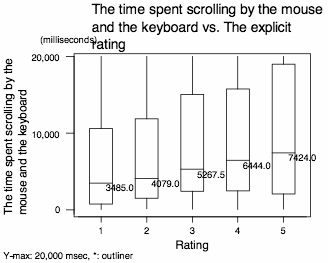
\includegraphics[width=7.5cm]{image/scrollgrey.jpg}
  \caption{Time spent scrolling, source: \citet{claypool2001}}
  \label{pic:scrolltime}
\end{figure}
\begin{figure}[h]
  \centering
  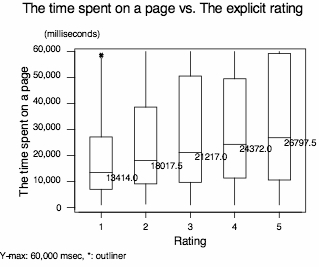
\includegraphics[width=7.5cm]{image/timegrey.jpg}
  \caption{Time spent on a page, source: \citet{claypool2001}}
  \label{pic:time}
\end{figure}

The two diagrams of figure~\ref{pic:scrolltime} and figure~\ref{pic:time} represent the time a user scrolls on a website and the time a user spends on a website.
These diagrams are created by the team of \citet{claypool2001}.
The x-axis represents the explicit user ratings and the y-axis represents the time a user has scrolled on a website and the time that a user has spend on the website respectively.
The bar for each explicit rating represents the time range of all users that explicitly rated the page with a rating of 1 (resp. 2, 3, 4 or 5).
The line in each of the bars represents the average time of all user times of that rating.
Interesting to note is that the average times for ratings in both diagrams have a steady rise which mirrors the statement of \citet{claypool2001} that these times correspond with the rating of the users.
However, the ranges of the ratings are very wide and thus for calculating the ratings from the times one should remove a percentage of the highest time that a user spends or scrolls as well as a percentage of the lowest times.
This process should filter the abnormal user times and yield data that should reflect the user interest more explicit.
This filtered data can now be used in order to calculate the average time of all users this process is called \emph{Truncated Mean} [\citet{wiki:truncated}].

%In order to collect implicit user ratings by timing how long the website is in focus, the truncated mean time all users spend on the item page is used as a benchmark.
\begin{definition}[Truncated Mean]
  The truncated mean (tm) is calculated the same way as the average mean after discarding a specific percentage of the highest and lowest values.
  Let $n \in \mathbb{N}$, V be a set of sorted numbers and p be a percentage with $0 \leq p < 0.5$.
  Let $k = np$ be the trimmed value, $r = n - 2k$ be the remaining values, $v_j \in V$ and $j \in \mathbb{N}$.
  Then the following formula represents the truncated mean.
  \begin{displaymath}
    tm = \sum_{j=k+1}^{n-k}{v_j} \cdot \frac{1}{r}
  \end{displaymath}
\end{definition}
% The percentages of the two rating processes result out of the two diagrams of figure ~\ref{pic:scrolltime} and figure ~\ref{pic:time}. 
% These diagrams are created by the team of \citet{claypool2001}.
% The x-axis represents the explicit user ratings and the y-axis represents the time a user has scrolled on a website and the time that a user has spend on the website respectively.
% The bar for each explicit rating represents the time range of all users that explicitly rated with that rating.
% The line in each of the bars represents the average time of all user times of that rating.
For this thesis the time differences between the average times of each rating which can be seen in figure~\ref{pic:scrolltime} and figure~\ref{pic:time} are assumed as a range for implicit ratings.
These ranges are expressed as percentages in dependence to the general average time of all users in the following two enumerations. 
%zeitliche abstaende zwischen den average ratings wurden als bereich fuer ein explicites rating angenommen und dieses wurde in abhaengigkeit zur gesamten average time prozentual ausgedrueckt
\begin{itemize}
  \item If the user spends up to 76.5\% of the truncated mean time on the item page it is used as a rating of 1.
  \item If the user spends between 76.5\% and 94.3\% of the truncated mean time on the website it is used as a rating of 2.
  \item If the user spends between 94.3\% and 109.6\% of the truncated mean time on the item page, it is used as a rating of 3.
  \item If the user spends longer than 109.6\% of the truncated mean time on the website it is used as a rating of 4.
\end{itemize}
%the largest range is the area from 0\% to 76.5\% which indicates a rating of one.
%
A rating of 5 can only be achieved if a user does a predefined user interaction on the web page such as clicking on a button that indicates interest.
The reason behind this choice is that users tend to make breaks while surfing the internet.
Thus, the user leaves the current browser window open but is not actively working on this website.
Therefore, it is possible that a user is on a break and the currently active browser window might not be interesting for him in that moment.
Such a predefined user interaction can be used as an indicator that a user likes an item.
A possible predefined user interaction could be an up-vote or the writing of a comment or an answer. 
A similar scale is chosen for determining the rating of a user by the time a user scrolls.
\begin{itemize}
  \item If the user scrolls less than 69\% of the truncated mean time on the item page it is used as a rating of 1.
  \item If the user scrolls between 69\% and 86\% of the truncated mean time on the webpage it is used as a rating of 2.
  \item If the user scrolls between 86\% and 108\% of the truncated mean time on the webpage it is used as a rating of 3.
  \item If the user scrolls between 108\% and 129\% of the the truncated mean time on the website it is used as a rating of 4.
  \item If the user scrolls longer than 129\% of the truncated mean time on the website it is used as a rating of 5
\end{itemize}
Scrolling is an active process and the user has to be in front of the computer to be able to scroll therefore a rating of 5 is achievable in this method.\\
In these two enumerations it is noticeable that the largest percentage area is at the rating of one.
This can be explained by the fact that the user examines the overall website before he starts to evaluate the content of the website.
Therefore the area of the rating of one contains the time that the user needs to make himself familiar with the website as well as the time he needs to evaluate the content.
For the calculation of the complete rating both implicit ratings - the time a user spends on a website and the time a user scrolls - are determined separately.
Afterwards the average of both ratings is calculated and used as the complete rating.
\begin{displaymath}
  complete Rating = \frac{rating_{time} + rating_{scroll}}{2}
\end{displaymath}
If a user returns to an item site the time that the user spends on the page and the time the user scrolls on the page is added to the previous times.
The sum of both sessions is used to calculate the new rating.
Consequently, a website which a user visits frequently generates a high rating.

\newpage
As mentioned above the research group of \citet{claypool2001} bases its results on a field experiment of over 80 people browsing over 2500 web pages.
The complete rating concept is strongly build upon these results.
It would have been desirable to conduct a field experiment for the newly developed concept of the complete rating but unfortunately due to the lack of time it was not possible.
%To get back to the original problem of computing the rating for an item based on the user interaction on a website
%describe the google news approach, explain the changes that where made and why.

%%source of definitions
%%why start with finite automata why create deterministic finite automata and how
\newpage
\section{Tagging}
In order to recommend items with a matching subject on a website, the newly developed system needs to be able to filter the items based on their content.
Therefore the keywords of the item content are used as tags in order to reflect the subject of the items. 
%The content can be described with the use of tags, these tags are the keywords of the content.
In the context of economics the \emph{Deutsche Zentralbibliothek f�r Wirtschaftswissenschaften Leibniz-Informationszentrum Wirtschaft} (ZBW) provides the \emph{STW Thesaurus for Economics} (STW).
The STW provides vocabulary on any economic subject and includes about 19000 terms and 6000 standardized keywords which can be used to match words from a text.\footnote{STW Thesaurus for Economics url: http://zbw.eu/stw/versions/latest/about}
It, thus, provides a good basis for the tagging process.
However, the STW only includes the basic form of the words while excluding most of the words with affixation, due to this it is not sufficient to check whether the words from the items are equal to the words from the STW.
It is not sufficient because many words would not match if they are in a different form or have spelling mistakes.
So, the challenge for this tagging process is to find the correct words in the STW even though the words from the item might not correspond directly to the words in the STW.
One possible solution for such a task is to reduce each word from the text to its stem.
According to \citet{englishLinguistics} a stem is the lexical unit that remains when all inflectional affixes are taken away.
Whereby, inflectional affixes are affixes that produce a new word form without changing the core meaning of the word.
Such an inflectional affix is for example the adding of the plural \emph{s} to a word.
Such a task is called stemming and is usually done by using predefined rules on the words. 
A rule is usually a combination of the minimum number of letters in a word, plus the suffix that should be changed and the replacement for the suffix.
More advanced algorithms might also use rules for prefix reduction and detecting irregular changes of the stem according to \citet{germanStemming}.
For example a predefined rule might be '3+ies' $\rightarrow$ 'y'.
So, the word \emph{libraries} would be transformed to \emph{library}.
Thus, it is important that the stemming algorithm has all necessary rules for each supported language which momentarily are English and German.\\
Another challenge for using the stemming algorithm is that all words in the basis for the tagging process must be in the stem form. 
Otherwise the algorithm might reduce a word to its stem that would actually match already in its original form.
Additionally a stemming algorithm cannot find words if they have spelling mistakes.
Because of these maintenance problems it was decided that the stemming algorithm is not suitable for the developed system.
Another possible solution for the problem is to calculate the number of changes that have to be done in order to transform the word from the text to the word from the basis for the tagging process.
%Another possible solution for the problem is to calculate the differences between the words from the text and the words from the basis for the tagging process.
This number can be used as an indicator whether the words are similar or not.
If they are in a predefined difference range the words can be used as tags.
This creates the need for a metric that indicates the difference or distance between two words.
A well known metric for such a task is the \emph{Levenshtein distance} which will be used in the system and will be explained in the following section.
\subsection{Levenshtein Distance}

The Levenshtein distance calculates the minimum numbers of substitutions, insertions and deletions that are needed to change one word into another[\citet{wiki:levenshteinDistance}].
The following example explains the Levenshtein distance for the words \emph{library} and \emph{libraries}.
The algorithm has to perform two deletions and one substitution in order to create the word \emph{library} out of the word \emph{libraries}.
If it creates the word \emph{libraries} out of the word \emph{library} it has to perform a substitution and two insertions.
\begin{displaymath}
  {library \leftrightarrow librari \leftrightarrow librarie \leftrightarrow libraries}
\end{displaymath}
Both processes result in a Levenshtein distance of three.
So, the Levenshtein distance is zero if the words are equal and adds one to the result if it has to perform a substitution, an insertion or a deletion of a letter. 
For a more detailed description compare algorithm~\ref{alg:levDist}.
%   $levDist_{a,b}(i,j) = $
%   \begin{cases}
%     max(i,j) \quad \quad \quad \quad \quad \quad \quad \quad \quad \quad \quad \quad \quad \quad \text{if min(i,j) = 0} \\
%     min \begin{cases}
%         levDist_{a,b}(i-1, j)+1 \\
%         levDist_{a,b}(i, j-1)+1 & \text{else}\\
%         levDist_{a,b}(i-1, j-1) + [a_i \neq b_i] 
%       \end{cases}
%   \end{cases}\\
% This can be directly translated into a recursive algorithm. 
\begin{algorithm}
  \caption{Recursive Levenshtein Distance Algorithm}\label{alg:levDist}
  \begin{algorithmic}[1]
    \Procedure{LevenshteinDistance}{$s: String, t: String$}
    \State $lenS\gets length(s)$
    \State $lenT\gets length(t)$
    \If{lenS = 0}
      \State \textbf{return} $lenT$
    \EndIf
    \If{lenT = 0}
      \State \textbf{return} $lenS$
    \EndIf

    \If{s[lenS-1] = t[lenT-1]}\Comment{test if last characters of the strings match}
      \State $cost\gets 0$
    \Else
      \State $cost\gets 1$
    \EndIf

    \Comment{The first recursive call represents a deletion, the second represents an insertion and the third represents a substitution or a correct letter}
    \State \textbf{return} minimum of\par
    $LevenshteinDistance(s[0..lenS-1], t) +1,$\par 
    $LevenshteinDistance(s, t[0..lenT-1) +1,$\par 
      $LevenshteinDistance(s[0..lenS-1], t[0..lenT-1]) + cost)$ 

    \EndProcedure
  \end{algorithmic}
\end{algorithm}



The direct implementation of the Levenshtein distance algorithm has a complexity of O(mn) with m being the size of the first word and n being the size of the second word. 
Therefore it is a good utility to better understand the Levenshtein distance in general, but it is not feasible for a software that should work in production mode. 

For finding the keywords for a text it is not necessary to know the Levenshtein distance for each word.
It is important to know if two words are in a pre defined range and, thus, be able to tell that these words are similar.
So, the next section explains the concept of a Levenshtein distance automaton which can decide in linear time whether two words are in a specific Levenshtein distance.

\subsection{Optimized Levenshtein distance algorithm}
%definitions
The following definitions are based on the book \emph{Introduction to automata theory, languages, and computation} by \citet{automata2003}.
\begin{definition}[Non Deterministic Finite Automata]
  A non deterministic finite automaton is a 5-tupel of the form $\mathcal{A} = (Q, \Sigma, q_0, \Delta, F)$. 
  \begin{itemize}
    \item Q is a finite set of the states
    \item $\Sigma$ is a finite set of input symbols
    \item $q_0 \in Q$ is the initial state
    \item $\Delta$ is a relation of the form $\Delta \subset Q \times \Sigma \times Q$
    \item $F \subset Q$ is a subset that contains the final states
  \end{itemize}
  $\mathcal{A}$ is called finite if and only if $Q$ is finite. Furthermore $\Sigma^*$ is the set of words over $\Sigma$ and $\epsilon$ is the empty word.
\end{definition}
\begin{definition}[Deterministic Finite Automata]
  $\mathcal{A}$ is deterministic if for all $p \in Q$ and all $a \in \Sigma$ exists exactly one state $q \in Q$ with $(p, a, q) \in \Delta$. In this case $\Delta$ is written as a function $\delta : Q \times \Sigma \rightarrow Q$.
\end{definition}
\begin{definition}[Path]
  A path for $\mathcal{A}$ is a series $\pi = p_0 a_1 p_1 a_2 \dots a_n p_n$ with $(p_i, a_{i+1}, p_{i+1}) \in \Delta$, $0 \leq i \leq n-1$ and $n \in \mathbb{N}$.
  The function $\beta(\pi)$ maps a path $\pi$ to a word $\omega \in \Sigma^*$.
  The length of $\pi$ is n and the label for $\beta(\pi)$ is $a_1 a_2 a_3 \dots a_n$.
\end{definition}
\begin{definition}[Path shortwriting]
  $\mathcal{A}: p \xrightarrow[]{\omega} q$ with $\omega \in \Sigma^*$ states that a path $\pi$ for $\mathcal{A}$ from p to q with label $\beta(\pi) = \omega$ exists.
\end{definition}
\begin{definition}[Automata accepts a word]
  $\mathcal{A}$ accepts $\omega \in \Sigma^*$, if and only if $p \in Q$ and $q \in F$ exists with $\mathcal{A}$: $p \xrightarrow[]{\omega} q$. For $\mathcal{A}$ let $\mathcal{L}(\mathcal{A})=\{\omega \in \Sigma^*$ | $\mathcal{A}$ accepts $\omega\}$ be the language that $\mathcal{A}$ accepts.
\end{definition}

The following definitions are based on \citet{schulz2002}
\begin{definition}[Formal Levenshtein Distance]
  The Levenshtein distance between two words $V, W \in \Sigma^*$ is the minimal number of edit operations (substitutions, deletions or insertions) that are needed to transform V into W.
  $d_L(V,W)$ denotes the Levenshtein distance between V and W.
\end{definition}
\begin{definition}
  $\mathcal{L}_{Lev}(n, W)$, $n \in \mathbb{N}$ and $W \in \Sigma^*$ is the set that denotes all words $V \in \Sigma^*$ such that $d_L(W,V) \leq n$.
\end{definition}

\begin{definition}[Degree Levenshtein Automata]
  Let $W \in \Sigma^*$ and $n \in \mathbb{N}$. A finite state automaton $\mathcal{A}$ is a Levenshtein automaton of degree n for W if and only if $\mathcal{L}(\mathcal(A)) = \mathcal{L}_{Lev}(n,W)$.
\end{definition}

An optimized version of the Levenshtein distance algorithm that uses a Levenshtein automaton is described by \citet{Baeza-Yates96aunified}.
The purpose of the Levenshtein automaton is to decide whether $d_L(W,V)$ with $W,V \in \Sigma^*$ is smaller than a specific $n \in \mathbb{N}$.
So, it is possible to decide if a word from a question is similar to a word from the STW, similar in the meaning it has a Levenshtein distance smaller than n.
Therefore $\Sigma$ contains the alphabet \{a, \ldots, z, A, \ldots, Z\}.
The states in Q of the Levenshtein automaton denote the current position in the original word W, written as i and the current Levenshtein distance between $\omega$ and W, written as j, with $\omega$ prefix of V.
The label of such a state is $i^j$.
Thus the initial state $q_0 \in Q$ is $0^0$.
The final states $f \in F$ are all states where i equals |W| and j is smaller or equal to n.\\
Let $\omega_{correct}$ be the correct letter after state $i^j$.
The relation $\Delta: (Q \times \Sigma \times Q)$ has the following elements:
\begin{itemize}
  \item $(i^j, \sigma, (i+1)^j)$ if $\sigma = \omega_{correct}$ 
  \item $(i^j, \sigma, i^{(j+1)})$ if $\sigma$ is inserted after state $i^j$ and $(j+1) \leq n$
  \item $(i^j, \sigma, (i+1)^{(j+1)})$, if $\sigma$ is substituted by $\omega_{correct}$ and $(j+1) \leq n$
  \item $(i^j, \epsilon, (i+1)^{(j+1)})$, if $\omega_{correct}$ is deleted
\end{itemize}
The elements are not exclusive therefore all of these cases can be possible after reading only one letter.
% \begin{math}
% (i^j, \sigma) \rightarrow \begin{cases}
%   (i+1)^j & \text{if correct}\\
%   (i)^{(j+1)} & \text{if insertion}\\
%   (i+1)^{(j+1)} & \text{if substitution or deletion}\\
%   empty & \text{if j is equal to n}
% \end{cases}
% \end{math}

\begin{figure}[h]
  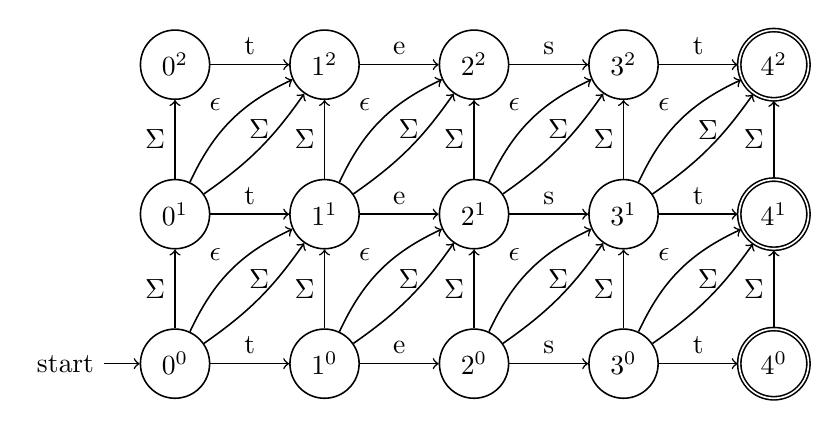
\begin{tikzpicture}[->,auto,line width=0.2mm] 
    %0,0 row
    \node[state] (q_2) {$0^2$}; 
    \node[state] (q_1) [below =of q_2] {$0^1$}; 
    \node[state,initial] (q_0) [below =of q_1] {$0^0$}; 

    %1,0 row t
    \node[state] (q_5) [right =of q_2] {$1^2$}; 
    \node[state] (q_4) [right =of q_1] {$1^1$}; 
    \node[state] (q_3) [right =of q_0] {$1^0$}; 

    %2,0 row e
    \node[state] (q_8) [right =of q_5] {$2^2$}; 
    \node[state] (q_7) [right =of q_4] {$2^1$}; 
    \node[state] (q_6) [right =of q_3] {$2^0$};

    %3,0 row s
    \node[state] (q_11) [right =of q_8] {$3^2$}; 
    \node[state] (q_10) [right =of q_7] {$3^1$}; 
    \node[state] (q_9) [right =of q_6] {$3^0$};

    %4,0 row t
    \node[state, accepting] (q_14) [right =of q_11] {$4^2$}; 
    \node[state, accepting] (q_13) [right =of q_10] {$4^1$}; 
    \node[state, accepting] (q_12) [right =of q_9] {$4^0$};

    %path deletion 0,0
    \path[->] 
    (q_0) edge node {$\Sigma$} (q_1)
    (q_1) edge node {$\Sigma$} (q_2);
    %path 0,0 -> 1,0
    \path[->] 
    %correct path
    (q_0) edge  node {t} (q_3)
    (q_1) edge  node  {t} (q_4)
    (q_2) edge  node  {t} (q_5)

    %insertion substitution
    (q_0) edge[bend right=10]  node[above,midway] {$\Sigma$} (q_4)
    (q_0) edge[bend left=20]  node  {$\epsilon$} (q_4)


    (q_1) edge[bend right=10]  node[above,midway] {$\Sigma$} (q_5)
    (q_1) edge[bend left=20]  node  {$\epsilon$} (q_5);

    %path deletion 1,0
    \path[->] 
    (q_3) edge node {$\Sigma$} (q_4)
    (q_4) edge node {$\Sigma$} (q_5);

    %path 1,0 -> 2,0
    \path[->] 
    %correct path
    (q_3) edge  node {e} (q_6)
    (q_4) edge  node  {e} (q_7)
    (q_5) edge  node  {e} (q_8)

    %insertion substitution
    (q_3) edge[bend right=10]  node[above,midway] {$\Sigma$} (q_7)
    (q_3) edge[bend left=20]  node  {$\epsilon$} (q_7)


    (q_4) edge[bend right=10]  node[above,midway] {$\Sigma$} (q_8)
    (q_4) edge[bend left=20]  node  {$\epsilon$} (q_8);


    %path deletion 2,0
    \path[->] 
    (q_6) edge node {$\Sigma$} (q_7)
    (q_7) edge node {$\Sigma$} (q_8);

    %path 1,0 -> 2,0
    \path[->] 
    %correct path
    (q_6) edge  node {s} (q_9)
    (q_7) edge  node  {s} (q_10)
    (q_8) edge  node  {s} (q_11)

    %insertion substitution
    (q_6) edge[bend right=10]  node[above,midway] {$\Sigma$} (q_10)
    (q_6) edge[bend left=20]  node  {$\epsilon$} (q_10)


    (q_7) edge[bend right=10]  node[above,midway] {$\Sigma$} (q_11)
    (q_7) edge[bend left=20]  node  {$\epsilon$} (q_11);

    %path deletion 3,0
    \path[->] 
    (q_9) edge node {$\Sigma$} (q_10)
    (q_10) edge node {$\Sigma$} (q_11);

    %path 3,0 -> 4,0
    \path[->] 
    %correct path
    (q_9) edge  node {t} (q_12)
    (q_10) edge  node  {t} (q_13)
    (q_11) edge  node  {t} (q_14)

    %insertion substitution
    (q_9) edge[bend right=10]  node[above,midway] {$\Sigma$} (q_13)
    (q_9) edge[bend left=20]  node  {$\epsilon$} (q_13)


    (q_10) edge[bend right=10]  node[above,midway] {$\Sigma$} (q_14)
    (q_10) edge[bend left=20]  node  {$\epsilon$} (q_14);

    %path deletion 3,0
    \path[->] 
    (q_12) edge node {$\Sigma$} (q_13)
    (q_13) edge node {$\Sigma$} (q_14);


  \end{tikzpicture}
  \caption{A non deterministic Levenshtein automaton for the word \emph{test} with degree 2}
  \label{ndla}
\end{figure}
The automaton in example~\ref{ndla} is a non deterministic Levenshtein automaton for the word \emph{test} with degree two.
So, it accepts all words that have a maximum distance of two to the word \emph{test}.
For example if the automaton reads the word \emph{tex} it can use the transition with the label \emph{t} which starts at the start state $0^0$ and ends in the state $1^0$.
The next letter \emph{e} can change the state from $1^0$ to $2^0$.
The following letter \emph{x} from the word \emph{tex} can substitute the letter \emph{s} from the original word \emph{test} by using the transition with the label \emph{$\Sigma$} from $2^0$ to $3^1$.
Finally, the last letter from the original word \emph{test} is deleted without reading a letter by using the $\epsilon$ transition from state $3^1$ to state $4^2$.
The state $4^2$ is a final state and, thus, the word \emph{tex} is accepted by this Levenshtein automaton.
In the following description the Levenshtein automaton represents the word $W \in \Sigma^*$ and $\sigma \in \Sigma$ is the currently read letter.
$\Sigma$ indicates that any element from $\Sigma$ is accepted on this path.
The initial state $0^0$ is in the bottom left corner.
If $\sigma$ is a correct letter it follows the horizontal path in the automaton.
A vertical path is an insertion of a letter $l \in \Sigma$ into the word W which is possible for any $\sigma$.
A diagonal path can be a deletion of a letter $l \in W$ with the empty word $\epsilon$ or a substitution of $\sigma$ for the currently correct letter in W. 
Therefore after reading the letter \emph{t} in the initial state $0^0$ the automaton can be in seven different states namely $0^1$, $1^2$, $1^1$, $2^2$, $1^0$, $2^1$ and $3^2$.
These seven different states can be reached because the \emph{t} is included in the alphabet $\Sigma$ and therefore the vertical transition for inserting a letter as well as the diagonal transition for substituting a letter can be chosen.
Additionally the $\epsilon$ transition which represents the deletion of a letter can be used at all times.
Finally the horizontal path can be used because \emph{t} is the correct letter for the current state.
Moreover from each destination of a transition the $\epsilon$ transitions can be used as well.
Yielding the seven different sates that were mentioned above.
Evaluating a non deterministic Levenshtein automata is computational complex due to the fact that there can be a large number of active states at the same time. 
Thus it is necessary to convert a non deterministic automata to a deterministic automata before using it to find tags.
The process of generating a deterministic automata with a non deterministic automata is called \emph{powerset construction}.

\subsubsection{Powerset Construction}
The process of creating a deterministic Levenshtein automata out of an non deterministic Levenshtein automata is based on the powerset construction from the book \emph{Introduction to Automata Theory, Languages, and Computation} by \citet{automata2003}.
Given a non deterministic Levenshtein automaton the construction of an equivalent deterministic Levenshtein automaton is described below. 
\begin{itemize}
  \item Create $q_0'$ as a set with original $q_0$ and all states that are reachable with an $\epsilon$ path.
  \item $Q' \subseteq 2^Q$, thus all $q \in Q'$ are subsets of Q.
  \item $\delta(R,a) = \{q \in Q$ | $\exists r \in R$ with (r, a, q) $\in \Delta$ or (r, a, p) and (p, $\epsilon$, q) $\in \Delta$ or (r, $\epsilon$, p) and (p, a, q) $\in \Delta\}$ whereby $R \subseteq Q$.  
  \item F' includes all $q \in Q'$ that include $f \in F$
\end{itemize}
Therefore the new deterministic Levenshtein automaton is (Q', $\Sigma$, $q_0'$, $\delta$, F').
\newpage


\begin{figure}[h]
  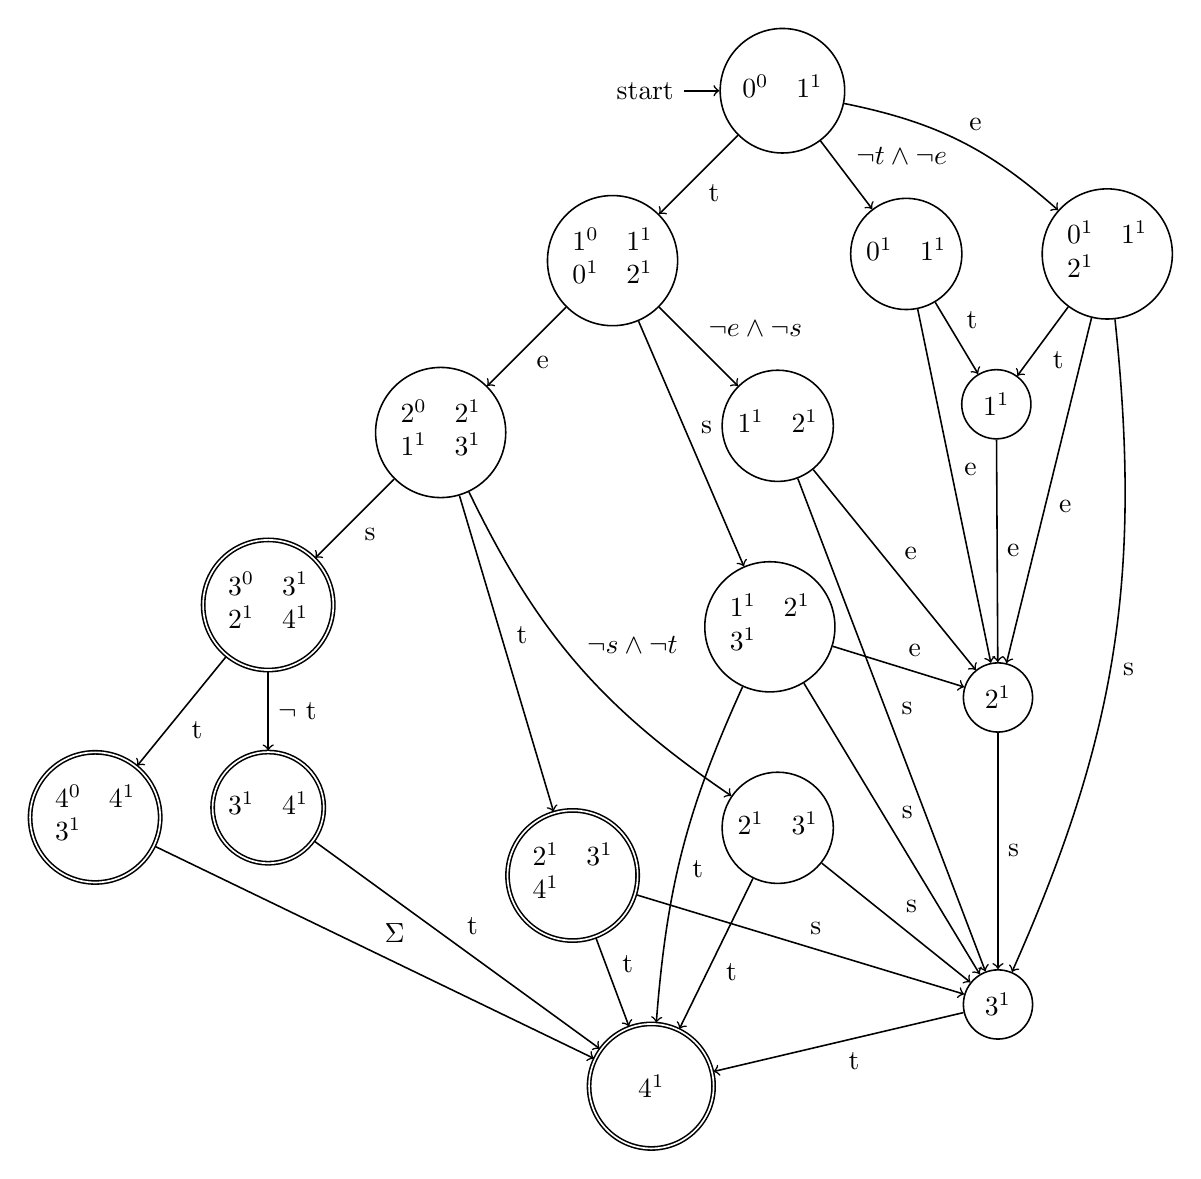
\begin{tikzpicture}[->,auto,line width=0.2mm] 
    \node[state,initial, minimum size=4.5em] (0_0-1_1) {$\begin{matrix} 0^0 & 1^1 \end{matrix}$}; 
    %correct path
     \node[state] (1_0-1_1-0_1-2_1) [below left=of 0_0-1_1] {$\begin{matrix} 1^0 & 1^1\\ 0^1 & 2^1 \end{matrix}$}; 
     \node[state] (2_0-2_1-1_1-3_1) [below left=of 1_0-1_1-0_1-2_1] {$\begin{matrix} 2^0 & 2^1\\ 1^1 & 3^1 \end{matrix}$}; 
     \node[state, accepting] (3_0-3_1-2_1-4_1) [below left=of 2_0-2_1-1_1-3_1] {$\begin{matrix} 3^0 & 3^1\\ 2^1 & 4^1 \end{matrix}$}; 

     \node[state, accepting] (4_0-4_1-3_1) [below left=of 3_0-3_1-2_1-4_1, yshift=-0.5cm] {$\begin{matrix} 4^0 & 4^1\\ 3^1 \end{matrix}$}; 

     %first not t,e
     \node[state] (0_1-1_1) [below right=of 0_0-1_1, xshift=-0.5cm] {$\begin{matrix} 0^1 & 1^1\end{matrix}$}; 

     %first e
     \node[state] (0_1-1_1-2_1) [right=of 0_1-1_1] {$\begin{matrix} 0^1 & 1^1\\ 2^1 \end{matrix}$}; 

      %q1 edges
     \node[state] (1_1-2_1) [below right=of 1_0-1_1-0_1-2_1] {$\begin{matrix} 1^1 & 2^1 \end{matrix}$}; 
     \node[state] (1_1-2_1-3_1) [below =of 1_1-2_1, xshift=-0.1cm] {$\begin{matrix} 1^1 & 2^1 \\ 3^1 \end{matrix}$}; 

     %elementar
     \node[state] (1_1) [below left=of 0_1-1_1-2_1, xshift=0.5cm] {$1^1$}; 
     \node[state] (2_1) [below right=8em of 1_1-2_1-3_1, yshift=2cm] {$2^1$}; 
     \node[state] (3_1) [below =of 2_1, yshift=-2cm] {$3^1$}; 



     \node[state, accepting] (3_1-4_1) [below =of 3_0-3_1-2_1-4_1] {$\begin{matrix} 3^1 & 4^1 \end{matrix}$}; 

     \node[state] (2_1-3_1) [below =of 1_1-2_1-3_1, xshift=0.1cm] {$\begin{matrix} 2^1 & 3^1 \end{matrix}$}; 
     \node[state, accepting] (2_1-3_1-4_1) [below left=of 2_1-3_1, xshift=-0.5cm, yshift=1.5cm] {$\begin{matrix} 2^1 & 3^1\\ 4^1 \end{matrix}$}; 
     \node[state, accepting, minimum size=4.5em] (4_1) [below =of 2_1-3_1-4_1, xshift=1.0cm, yshift=-0.5] {$4^1$}; 
     \path[->]
     (0_0-1_1) edge node {$\neg t \wedge \neg e$} (0_1-1_1)
     (2_0-2_1-1_1-3_1) edge[bend right=15] node {$\neg s \land \neg t$} (2_1-3_1)
     (2_0-2_1-1_1-3_1) edge node {t} (2_1-3_1-4_1)
     (0_0-1_1) edge[bend left=15] node {e} (0_1-1_1-2_1)
     (1_0-1_1-0_1-2_1) edge node {$\neg e \wedge \neg s$} (1_1-2_1)
     (1_0-1_1-0_1-2_1) edge node {s} (1_1-2_1-3_1)
     (0_1-1_1) edge  node {t} (1_1)
     (0_1-1_1) edge  node[bend right=15] {e} (2_1)
     (1_1) edge  node {e} (2_1)
     (2_1) edge  node {s} (3_1)
     (3_1) edge  node {t} (4_1)
     (1_1-2_1) edge  node {e} (2_1)
     (1_1-2_1) edge  node {s} (3_1)
     (3_0-3_1-2_1-4_1) edge node {$\neg$ t} (3_1-4_1)
     (3_1-4_1) edge node {t} (4_1)
     (0_0-1_1) edge  node {t} (1_0-1_1-0_1-2_1)
     (1_0-1_1-0_1-2_1) edge  node  {e} (2_0-2_1-1_1-3_1)
     (2_0-2_1-1_1-3_1) edge  node  {s} (3_0-3_1-2_1-4_1)
     (3_0-3_1-2_1-4_1) edge  node  {t} (4_0-4_1-3_1)
     (2_1-3_1-4_1) edge  node {t} (4_1)
     (2_1-3_1-4_1) edge  node {s} (3_1)
     (2_1-3_1) edge  node {s} (3_1)
     (2_1-3_1) edge  node {t} (4_1)
     (0_1-1_1-2_1) edge  node {t} (1_1)
     (0_1-1_1-2_1) edge  node {e} (2_1)
     (0_1-1_1-2_1) edge[bend left=15]  node {s} (3_1)
     (1_1-2_1-3_1) edge  node {e} (2_1)
     (1_1-2_1-3_1) edge  node {s} (3_1)
     (1_1-2_1-3_1) edge[bend right=10] node {t} (4_1)
     (4_0-4_1-3_1) edge  node  {$\Sigma$} (4_1);


  \end{tikzpicture}
  \caption{A deterministic Levenshtein automaton for the word \emph{test} with degree 1}
  \label{dla}

\end{figure}


% \begin{itemize}
%   \item $\Sigma$ is the complete alphabet
%   \item Each state in Q denotes for an insert word $\omega \in \Sigma^*$ the number of matching letters together with $d_L(\omega,W)$
%   \item The initial state $q_0$ is the state with insert count 0 and \emph{levenshtein distance} 0
%   \item The function $\delta$ is the known function $\delta : Q \times \Sigma \rightarrow Q$. 
%   \item The set of final states F contains all states where the correct letter count is equal to the size of the original word W.
% \end{itemize}

Let $(Q, \Sigma, q_0, \Delta, F)$ be a non deterministic Levenshtein automaton for the word \emph{test} with maximum Levenshtein distance 1\footnote{This is the automaton from figure~\ref{ndla} without the first row}. 
Then the deterministic Levenshtein automaton $DLA = (Q', \Sigma, q_0', \delta, F')$ from figure~\ref{dla} is the output from the powerset construction.
Consequently the DLA can only have one active state at a time and accepts all words V from $\Sigma^*$ with $d_L(test, V) \leq 1$. 
This deterministic finite automaton with degree $n \in \mathbb{N}$ for a word $W \in \Sigma^*$ can decide in linear time if a word $V \in \Sigma^*$ has $d_L(W,V) \leq n$ [\citet{schulz2002}. 


% \begin{algorithm}
%   \caption{Levenshtein Automaton is in distance}\label{alg:levDistIsInDist}
%   \begin{algorithmic}[1]
%     \Procedure{isInDistance}{$automata: DeterministicFiniteAutomata, term: String$}
%     \State $i\gets 0$
%     \State $currentStates\gets (0,0)$\Comment{add the initial state}
%     \While{currentStates.size > 0 AND i < term.length}
%       \State $c\gets term[i].toLowerCase$\Comment{c gets the current active lower cased letter}
%       \State $currentStates\gets automate.nextState(currentStates, c)$
%       \State $i\gets i+1$
%     \EndWhile
%     \If{currentStates includes a final state}
%       \State \textbf{return} true
%     \Else
%       \State \textbf{return} false
%     \EndIf

%     \EndProcedure
%   \end{algorithmic}
% \end{algorithm}

%Jetzt koennen fuer all woerter in einem item ein solcher deterministischen automaten erstellt werden.
%Allerdings kann nich fuer jeden automaten die gleiche degree verwendet werden, da ansonsten fuer ein kurzes word mit drei buchstaben eine distance von drei gewaehlt wird und somit alle woerter mit drei buchstaben matchen wuerden.
With this concept for each word in an item a deterministic Levenshtein automaton can be generated.
With the Levenshtein automaton it is decidable if a word is in a specific distance.
However, it is not a good approach to use the same distance for all words if for example the standard distance would be three then each word that has three or less letters would match with every other word of the same size yielding a lot of false matches.
Therefore there is a need for creating ranges for the degree of a Levenshtein automaton in dependence to the length of the word which is introduced in this thesis.
The most occurring change of a noun is the plural form.
The book \emph{German Noun Plural reconsidered} by \citet{thiessen2009pluralbildung} describes different forms of plural creation in the German language.
According to \citet{thiessen2009pluralbildung} the maximum number of letters that are appended as a suffix during the plural creation process for nouns is two.
These suffixes are \emph{-er} and \emph{en}.
However there are word forms that change the vowel into an umlaut during the plural creation process.
Therefore the maximum Levenshtein distance between a noun and its plural form is three.

The maximum distance for a given word $W \in \Sigma^*$ depends on the length n of W.
A word with a length of $n\leq 3$ in the STW is usually an abbreviation and therefore is only used as a direct match.
A word with a length of $3<n\leq 5$ is used with a maximum distance of one.
Therefore all noun plural forms that are created with the appending of one suffix are matched as well as spelling mistakes with a distance of one but the cases with a distance of more than one character are not matched.
This choice is made because a Levenshtein distance of more than one would yield too many false matches for such short words.
A word with a length of $6\leq n$ is used with a maximum distance of three.
Thus, all plural forms that are created for a word with five or more letters are matched.
If the stem of a word has five letters a plural form would add at least one additional letter and therefore the word would have at least six letters.
This would create a deterministic Levenshtein automaton with a degree of three for this word which would match all plural forms.
%Maskulina und Neutra mit er-Plural 3 aenderungen Wurm Wuermer
%substantive mit er plural beisplie Fass Faesser

%optimization generate dfa directly or use table based evaluation method

%Lemma 6 For any fixed number n, given two words W and V of length w and v respectively, it is decidable in time O(max(w, v)) if the Levenshtein distance between W and V is <= n.

To get back to the original problem this paragraph explains the application of a Levenshtein distance automata to find the right tags for a text.
The overall tagging concept is to calculate for every word from the text an automaton based on the length of the word and read all words from the STW into each automata.
If a word from the STW ends in a final state it is used as a tag for the text. 
A possible optimization would be to calculate all the automata once for the complete STW and to store it with an efficient data structure in a database.
Currently the STW is stored in a triple store because it can easily be updated with the standard files from the website.
A triple store is a special database that stores data in the form of triples.
The triple store technology is described in more detail in subsection 3.1.2.

\newpage
%why did I choose item-based and svd-based recommendations? why the combination of both
%description of item based recommendation, how do I use item based recommendations
%description of collaborative filtering, description of svd, how do I use this sort of recommendations
\section{Recommendation}
A recommendation system is a system that creates personalized item recommendations based on information about the items or the relation between items and users.
These recommendations can be created by different types of recommendation systems that exploit different information about the users or items.
\subsection{Different types of recommendation systems}
The book \emph{Recommender Systems An Introduction} by \citet{recommender2011} distinguishes between the following four different kinds of recommendation systems.
%These recommendation systems that are described below exploit either the relationship between the users 
\subsubsection{Collaborative recommendation}
Collaborative recommendations are recommendations based on similar interests of users.
So, if user A and user B are interested in similar items and user A shows interest in item I that is unknown to user B than item I might be interesting for user B as well.
Because this technique filters all items based on implicit collaboration of the users it is also known as \emph{collaborative filtering}.
For using the collaborative filtering approach no other information are needed than the relationship between users and items. 
Depending on the number of items in the system and the activity of the users of the system the process of collecting information about the relation between the users and the items they are interested in might be needing some time.
Although it needs some time to collect initial data in the beginning it generally is a good approach if the items that need to be recommended are unknown or additional information for the items would be hard to maintain.
\subsubsection{Content-based recommendation}
In content-based recommendations the items are usually documents that should be recommended based on the content.
Thus, the content of the document is described by tags.
These tags can have an indicator that expresses the importance of the tag.
Therefore the documents can be filtered by the tags of the documents and ranked by the importance of those tags.
These tags can be maintained explicitly by the users of the systems or by tagging algorithms.
One advantage of content-based recommendation systems is that they do not require a large user base to achieve good recommendations for users.
A second advantage is that new items can be recommended to users immediately after the content has a description.
If the content is user generated the recommendation system can only recommend documents that fit the current context.
It has no information whether a user likes the content or not which can lead to poor recommendations.
All in all, content-based systems are a good choice if the system has to provide recommendations for quality documents.

\subsubsection{Knowledge-based recommendation}
A knowledge-based recommendation system is a system that has enough information about the items and the needs of the user and as such can recommend items based on matching the needs of the user and the features of the items.
Moreover the system has to use individual user requirements in order to create personalized recommendations. 
For example if a user would like to buy a new jacket for a summer camping trip in England the knowledge based system has to use the specific context in order to recommend a thin light rain jacket with the right size and price for the user.
These information are usually manually provided by the user and the maintainer of the system.
Furthermore not only the system needs to correctly interpret the information but the user needs to have the domain knowledge in order to provide the system with the correct information.
Consequently, knowledge-based recommendation is a good approach if the system has to recommend items that are not frequently requested and no user history is available.
It is especially suited for applications in which items are not frequently rated such as expensive digital goods or cars. 

% \subsubsection{Hybrid approaches}
% All recommendation system approaches have advantages and disadvantages, therefore a combinations of the different approaches which are mentioned above could improve the user recommendations as long as the system has enough information about the items or users.

\subsubsection{Conclusion}
%not enough information for knowledge based system
%use tags to filter collaborative recommendations
%fall back for cold start problem
%new user / not logged in
%use top rated items for the subject
%if no items 
%use top rated items
All of the described recommendation approaches have advantages and disadvantages.
Knowledge based systems require too much domain knowledge that is not accessible for user generated questions and answers and therefore knowledge based systems are not feasible for the implemented system.
On the other hand collaborative recommendation systems need an initial amount of user item relationship data in order to present good recommendations. 
Additionally, they have no information about the subject of the items and this might lead to a situation were a collaborative filtering system might recommend inappropriate items to the current context. 
Nonetheless collaborative filtering is the only approach that takes the interest of similar users into account. 
As such it is the only technique that is able to recommend items that are approved by similar users. 
Besides the content-based systems have the disadvantage that they do not make use of the information whether or not a user is interested in a document.
Thus they can only recommend items based on the context and are not able to recommend items that were interesting to other users in the past.
Therefore it is possible that a content-based system recommends user generated content of poor quality which is not desirable.
The user generated content of the implemented system is not moderated and therefore the system has no information about the quality of the content.
For that reason the implemented system uses a collaborative filtering technique with pre filtered content based on the tags for each item.
This approach should yield the best possible recommendations for a user of the system.

%%definitions Users, items, ratings, predictions
\newpage
\subsection{Collaborative recommendation system}
The following definitions are based on \citet{recommender2011}
\begin{definition}[User]
  $U = \{u_1, u_2, u_3, \dots, u_n\}$ is a set with $u_i$ being users from the recommendation system in which $n, i \in \mathbb{N}$ and $i \leq n$.
\end{definition}

\begin{definition}[Item]
  $I = \{i_1, i_2, i_3, \dots, i_n\}$ is a set with $i_j$ being items from the recommendation system in which $n, j \in \mathbb{N}$ and $j \leq n$.
\end{definition}

\begin{definition}[Rating]
  R is an $n \times m$ matrix with $n = |I|$ and $m = |U|$. 
  Furthermore $r_{n,m}$ is a rating for item $n \in I$ and user $m \in U$ with $r_{n,m}$ being an entry in R and $r_{n,m} \in \{1, 2, 3, 4, 5\}$.
  If a user $k \in U$ has not rated an item $l \in I$ the entry $r_{l, k}$ remains empty.
  $\hat{I_u}$ is a set with all items $i \in I$ in which $r_{i, u}$ is empty and $\tilde{I_u}$ is a set with all items i and $r_{i, u}$ is not empty.
\end{definition}

\begin{definition}[Prediction]
  A prediction is a rating $r_{i,u}$ for item $i \in I$ and user $u \in U$ with $r_{i,u}$ being an empty entry in $R$.
\end{definition}

\begin{definition}[Recommendation]
  Let $n \in \mathbb{N}$ and $u \in U$.
  A recommendation is a set of n predictions for a user u ordered by the values of the predictions.
\end{definition}


As mentioned above a collaborative recommendation system recommends items to users based on the interest of similar users.
Every collaborative recommendation technique can be divided into two different stages of calculations.
The first calculation stage is called \emph{offline calculation} in this thesis these include all calculations that are used to calculate the similarity between items or users.
The second calculation stage is called \emph{prediction calculation} in this thesis this stage includes all calculations that are used to calculate the rating predictions for a user-item pair.
The book \emph{Recommender Systems An Introduction} by \citet{recommender2011} differentiates between a number of different collaborative filtering techniques which are outlined below.
\subsubsection{User Based Nearest Neighbour Recommendations}
The user based nearest neighbour recommendation technique is one of the earliest collaborative recommendation methods.
It recommends items based on the similarity between users.
Therefore the similarity between each user is computed and the prediction for a user-item pair is calculated by using the most similar users that rated the item and multiplying the similarity of the users with the rating the result is normalized by the sum of all similarities of the users that were used.
%pearson found by harlocker to be the best formula to calculate the similarities between users
\subsubsection{Item Based Recommendations}
The item based recommendation method calculates rating predictions based on the similarity between the items.
Thus, it is similar to the user based nearest neighbour recommendation technique but it uses the similarity between the items instead of the similarity between the users to calculate the rating predictions.
\subsubsection{Singular Value Decomposition Recommendations}
The singular value decomposition recommendation technique can be used to derive a set of latent factors from the user-item rating matrix.
These latent factors can be used as vectors which can characterize users or items.
In the movie domain such a latent factor can correspond to obvious aspects of a movie such as the genre of the movie but it can also be uninterpretable.
The vectors of latent factors can be used for calculating the similarities between users.
Finally, these user similarities can be used for calculating the prediction for a user-item pair in the same manner that is used for the user based nearest neighbour recommendation technique.
\subsubsection{Probabilistic Recommendations}
The probabilistic recommendation technique creates groups of users and calculates the probability of group membership for each user.
If a prediction has to be calculated for a user $u \in U$ and an item $i \in I$ the probability that the group in which user u belongs is used to decide whether u likes item i or not.
However, the number of user groups and the maximum size of each group have to be evaluated for each use case depending on the prediction quality.

\subsubsection{Thesis Recommendation Approach}
The recommendation approach that is developed in this thesis is a combination of item based and matrix factorization recommendations.
In productive recommendation systems the user-item rating table is usually very sparse [\citet{recommender2011}].
That means that most users only rate a low number of items.
Thus, the rating matrix that is used for calculating the singular value decomposition has a lot of empty entries.
The idea behind the approach in this thesis is to predict the missing entries of the rating matrix with the item based recommendation approach.
Therefore, the singular value decomposition can be calculated with a matrix that provides more rating data.
Hence, the latent factors that are derived by the singular value decomposition should be more distinctive and should result in better user similarities. 
The following pages explain the item based recommendation technique and the recommendation technique based on the singular value decomposition in more detail.

% -different collaborative recommendation techniques
% -user based nearest neighbor recommendations
% --Memory based approach best similarity measure pearson correlation 
% -item based
% --recommends items based on similar items
% -matrix factorization techniques
% --uses matrix factorization techniques to get latent data that is hidden in the user item matrix this data is used to create recommendations
% -probabilistic recommendation
% --
% kombinieren von itembased und svd based recommendations to improve the rating matrix that is needed for the svd and thus generate better latent semantic factors that are used for calculating the similarity between the users
%There are different types of collaborative recommendation techniques.

\subsubsection{Item-Based Recommendation}
The concept of item-based recommendation was introduced by \citet{sarwar2001}.
The idea behind this concept is that recommendations can be calculated with the similarity between the items that are rated by a user and the items that the user has not rated.
If $i \in \hat{I_u}$ and $u \in U$, then the prediction for i can be calculated using the similarity between i and all items $j \in \tilde{I_u}$.
Researches made by \citet{sarwar2001} show that the \emph{adjusted cosine similarity} has the best performance with attention to prediction accuracy compared to all other similarity measures for item based algorithms. 
The adjusted cosine similarity is a special form of the \emph{cosine similarity} which is explained in the following definition for better understanding the adjusted cosine similarity.
The following definition of the cosine similarity is based on \citet{recommender2011}.
%However, \citet{sarwar2001} found out that the similarity calculation with the best performance is \emph{adjusted cosine similarity} which is an optimized form of the \emph{cosine similarity}.
\begin{definition}[Cosine Similarity]
  \label{cosineSimilarity}
  One has i, j $\in \mathbb{N}^n$, n $\in \mathbb{N}$ so that
  \begin{equation}
    cos(\overrightarrow{i}, \overrightarrow{j}) = \frac{\overrightarrow{i} \cdot \overrightarrow{j}}{||\overrightarrow{i}||_2 \cdot ||\overrightarrow{i}||_2} = \frac{\sum_{i = 1}^{n}\overrightarrow{a_i}\overrightarrow{b_i}}{\sqrt{\sum_{i = 1}^n \overrightarrow{a_i}^2} \sqrt{\sum_{i = 1}^n\overrightarrow{b_i}^2 }}
  \end{equation}
\end{definition}.
In general the results of the cosine similarity vary between -1 and 1.
However, the values of the vectors in the use case of the recommendation system are in the range of 1 to 5.
Therefore the vectors do not include negative values and the cosine similarity in the domain of the recommendation systems vary between 0 and 1.
According to \citet{recommender2011} results of the cosine similarity near to 1 mean strong similarity between the items.
If $\overrightarrow{i}$ and $\overrightarrow{j}$ are rating vectors, the individual rating behaviour of a user needs to be taken into account to improve the similarities between $\overrightarrow{i}$ and $\overrightarrow{j}$.
Because some users tend to rate items in general higher or lower than other users.
Yielding different average ratings for different users.
This results in the adjusted cosine similarity.
\begin{definition}[Adjusted Cosine Similarity]
  \label{adjustedCosine}
  Let $i,j \in I$(Items) and $\overline{r_u}$ be the average rating from user u.
  The cosine similarity can be transformed to the adjusted cosine similarity by subtracting the average user rating from the current rating.
  Let $\tilde{U}$ be all users that rated item i and item j.
  \begin{equation}
    sim(i, j) = \frac{\sum_{u \in \tilde{U}}{(r_{u, i} - \overline{r_u})(r_{u, j} - \overline{r_u})}}{\sqrt{\sum_{u \in \tilde{U}}(r_{u,i} - \overline{r_u})^2} \sqrt{\sum_{u \in \tilde{U}}(r_{u,j} - \overline{r_u})^2}}
  \end{equation}
\end{definition}
The results of the adjusted cosine similarity are between -1 and 1 with 1 meaning identical, 0 meaning indifferent and -1 meaning opposite [\citet{recommender2011}].
The user item predictions can be generated with the similarities by using the following formula which is based on \citet{recommender2011}.
\begin{definition}[Item Based Prediction]
  \label{itemPrediction}
  \begin{equation}
    pred(u, p) = \frac{\sum_{i \in \tilde{I_u}}{sim(i, p) \cdot r_{u, i}}}{\sum_{i \in \tilde{I_u}}{ sim(i, p)}}
  \end{equation}
\end{definition}
The item similarity calculations can be calculated offline on a regular basis - every day or weekly - depending on the activeness of the users and the amount of item changes.
So, the item based technique is a good choice for websites that need fast scalable recommendations because only the item predictions are calculated on time.
Furthermore the team of \citet{sarwar2001} found out that the system only needs a subset of all items.
According to \citet{sarwar2001} a sample of the 25 most similar items is needed to generate good recommendations.
Thus the on time calculation needs to find the top 25 most similar users in the similarity table and has to calculate the recommendations with these users instead of using all similar users.
Moreover, it is a tested concept for instance amazon.com uses item based recommendations for their product recommendations [\citet{amazon2003}]. 
To get back to the overall concept, the item based predictions are used in order to decrease the rating sparsity of the user-item table. 
Consequently, more information about the user's interest is available before the actual user similarities are calculated with the singular value decomposition which is explained in the following section.
In real world recommendation systems the user item ratings tend to be very sparse because most users only rate few items [\citet{recommender2011}].

\subsubsection{Example for Item-Based Recommendations}
The table in figure~\ref{itemBasedTable} represents a user item relationship.\\

\begin{table}[H]
  \centering
  \begin{tabular}{c c c c c c}
   &Item1 & Item2 & Item3 & Item4 & Item5 \\ 
  User1 & 5 & 3 & 4 & 4 & ?\\  
  User2 & 3 & 1 & 2 & 3 & 3\\ 
  User3 & 4 & 3 & 4 & 3 & 5\\ 
  User4 & 3 & 3 & 1 & 5 & 4\\ 
  User5 & 1 & 5 & 5 & 2 & 1\\ 
  \end{tabular}
  \caption{User Item Relationship Table}
  \label{itemBasedTable}
\end{table}

  This example calculates the item based prediction for User1 and Item5.
  For the adjusted cosine formula the average ratings for all users are needed.
  \begin{displaymath}
    \overline{r}_{User1} = \frac{\sum_{i \in \tilde{I}_{User1}}{r_{User1, i}}}{\sum_{i \in \tilde{I}_{User1}} 1} = \frac{5 + 3 + 4 + 4}{4} = 4.0
  \end{displaymath}
  The following average ratings are calculated analog.\\
  $\overline{r}_{User2} = 2.4$ \\
  $\overline{r}_{User3} = 3.8$ \\
  $\overline{r}_{User4} = 3.2$ \\
  $\overline{r}_{User5} = 2.8$ \\
  The following formula calculates the adjusted cosine similarity from definition~\ref{adjustedCosine} between Item5 and Item1.

  \footnotesize
  \begin{displaymath}
   sim(Item5,Item1) =
 \end{displaymath}
  \begin{displaymath}
    {{(3-2.4)\cdot(3-2.4) + (5-3.8)\cdot(4-3.8) + (4-3.2)\cdot(3-3.2) + (1-2.8)\cdot(1-2.8)} \over {\sqrt{(3-2.4)^2 + (5-3.8)^2 + (4-3.2)^2 + (1-2.8)^2} \cdot \sqrt{(3-2.4)^2 + (4-3.8)^2 + (3-3.2)^2 + (1-2.8)^2}}} = 
  \end{displaymath}
  \begin{displaymath}
    0.8040 
  \end{displaymath}
  \normalsize
  Similar to this calculation one computes the degree of similarity between Item5 and Item2, Item3 as well as Item4. 
  The results are shown below.\\
  sim(Item5, Item2) = -0.9082\\
  sim(Item5, Item3) = -0.7635\\
  sim(Item5, Item4) = 0.4330\\
  With these similarities the following prediction can be calculated using the item based prediction formula of definition~\ref{itemPrediction}.
  \begin{displaymath}
    pred(User1, Item5) = {{0.8040 \cdot 5 + (-0.9082) \cdot 3 + (-0.7635) \cdot 4 + 0.4330 \cdot 4} \over {0.8040 + (-0.9082) + (-0.7635) + 0.4330}} = 4.6501
  \end{displaymath}

  As a result User1 would most likely rate Item5 with 4.6501.

\subsubsection{Singular Value Decomposition}
The singular value decomposition is a matrix factorization technique that can be used to find latent factors in the rating patterns.
With these factors it is possible to find similar users and items.
The singular value decomposition was found in the late 1800 to early 1900 [\citet{historyOfSVD}].
% Besides one of the main areas of application of the singular value decomposition today is information retrieval.
% The basic idea behind the singular value decomposition based information retrieval is to match user queries to documents [\citet{deerwester1990}].
%This is done by decomposing a term by document matrix and using the item vectors of the decomposition to find documents based on queries that are decomposed into term vectors .
The following definitions are based on the book \emph{Linear Algebra Done Right} by \citet{axler1997linear}.
\begin{definition}[Linearly Dependent, Linearly Independent ]
  Let $v_1, v_2, \dots, v_n$ be a list of vectors in $\mathbb{R}^k$ whereby $k \in \mathbb{N}$.
  This list of vectors is called linear independent if the only possible solution of $a_1, a_2, a_3, \dots, a_m \in \mathbb{R}$ that makes $a_1v_1 + a_2v_2 + \dots + a_nv_n$ equal to 0 is $a_1 = \dots = a_n = 0$.
  A list of vectors is called linear dependent if they are not linear independent.
  In other words if at least one element of $a_1, a_2, a_3, \dots, a_m$ is not null such that $a_1v_1 + \dots + a_nv_n$
\end{definition}

\begin{definition}[Rank of a Matrix]
  The rank of a matrix A is the maximum number of linearly independent column vectors of A.
  For the reason that the rank of the linearly independent column vectors is always equal to the number of linearly independent row vectors it is also correct that the rank of matrix A is the maximum number of linearly independent row vectors of A.
\end{definition}
\begin{definition}[Unit Vector]
  A unit vector is a vector with length 1.
  Let $v \in \mathbb{R}^k$, $k \in \mathbb{N}$ and v is a unit vector then the following equation becomes true.
  \begin{displaymath}
    ||v|| = \sqrt{\sum_{i=1}^k{v_i^2}} = 1
  \end{displaymath}
\end{definition}
\begin{definition}[Orthogonal Vector]
  Two vectors are orthogonal if the dot product of those vectors is 0.
  Let $v, w \in \mathbb{R}^k$, $k\in \mathbb{N}$ and $v, w$ are orthogonal to each other then the following equation becomes true.
  \begin{displaymath}
    v \cdot w = \sum_{i = 1}^k v_i \cdot w_i = 0
  \end{displaymath}
\end{definition}
\begin{definition}[Orthogonal Matrix]
  An orthogonal matrix $A\in\mathbb{R}^k$ whereby $k\in\mathbb{N}$ is a quadratic, real matrix whose column and row vectors are pairwise orthonormal together.
  Furthermore is the inverse of the matrix equal to the transpose of the matrix.
  \begin{displaymath}
    A^{-1} = A^t
  \end{displaymath}
  Additionally the product of an orthogonal matrix with its transpose results the identity matrix.
  \begin{displaymath}
    AA^t = I
  \end{displaymath}
\end{definition}
\begin{definition}[Eigenvalue of a Matrix]
  An eigenvector of a square matrix A is a non-zero vector v that, when multiplied by A, yields the original vector multiplied by a single number $\lambda$; that is:
  \begin{displaymath}
    Av = \lambda v
  \end{displaymath}
  The number $\lambda$ is called the eigenvalue of A corresponding to v.
\end{definition}

The book \emph{Recommender Systems An Introduction} by \citet{recommender2011} describes the singular value decomposition (SVD) of an $m \times n$ matrix M with rank r as a factorization of the form:
\begin{displaymath}
  SVD(M) = U \Sigma V^t
\end{displaymath}
U and V are orthogonal matrices with dimension $m \times r$ and $r \times n$ respectively. 
Furthermore $\Sigma$ is a rectangular diagonal matrix with dimension $r \times r$.
The diagonal values $\sigma_{i,i} \in \Sigma$ with $i \in \mathbb{N}$ have by convention the property $\sigma_{i,i} \geq \sigma_{i+1,i+1} > 0$.
The $\sigma_{i,i}$ are the none negative square roots of the eigenvalues of $AA^t$ and $A^tA$ [\citet{numericalLinearAlgebra}]\footnote{$AA^t$ and $A^tA$ share the same eigenvalues.}. 
The columns of U are the corresponding eigenvectors to the eigenvalues of $AA^t$.
On the other hand the columns of the Matrix V are the corresponding eigenvectors to the eigenvalues of $A^tA$ [\citet{numericalLinearAlgebra}]\footnote{The eigenvalues are the squares of $\sigma_{i,i}$}.
This results in: $AA^t \cdot u_i = \sigma_{i,i}^2 \cdot u_i$ and $A^tA \cdot v_i = \sigma_{i,i}^2 \cdot v_i$.\\ 
So, the matrix U corresponds to the columns of the matrix A and the matrix V corresponds to the rows of the matrix A[\citet{Sarwar02incrementalsingular}].
It is possible to obtain an optimal rank k approximation from matrix A with $k \leq r$ by setting all $\sigma_{i,i}$ with $i > k$ to zero [\citet{matrixAlgorithms}].
Thus $A_k = U_k \Sigma_k V_k^t$ yields the optimal rank k approximation.
As a result, all column vectors $u_i$ with $i > k$, of matrix U will be multiplied by a zero vector from matrix $\Sigma_k$.
The matrix U represents the columns of matrix A and the last rows of matrix U will be removed in order to generate the optimal rank k approximation of matrix A, therefore it is possible to generate a good approximation of the user's interests by removing the last rows of matrix U\footnote{A user from the system is represented by a column in the matrix A}.
The two dimensional matrix $U_2$ is created by removing all rows of matrix U up to the first two rows.
This matrix $U_2$ can be seen as a value table that can be represented by a graph.
Therefore, it enables a graphical presentation of the user similarities.
Furthermore, the user similarities can be computed by using the cosine similarity between the columns of $U_k$.\\
After calculating the similarities for each user, the recommendations for $user_a \in U$ are calculated.
The following prediction calculation process is based on \citet{recommender2011}.
The prediction calculation algorithm takes all similar users $U_{sim}$ for $user_a$ and uses the top rated items from all $user_b \in U_{sim}$ that are not rated by $user_a$.
This is denoted by $I'_{user_a, user_b}$.
The average rating of user a is denoted by $\overline{r_a}$.
Finally for each item $i \in I'_{user_a, user_b}$ the prediction is calculated by using the following formula.

\begin{equation}
  \label{predictionSVD}
  pred_{a, i} = \overline{r_a} + \frac{\sum_{b \in U_{sim}}{(r_{i, b} - \overline{r_b}) * similarity_{a, b}}}{\sum_{b \in U_{sim}}{similarity_{a, b}}}
\end{equation}

% def getCalculateUserPredictions(userId: Int, path: Array[String]): Future[HttpResponse] = {
%   val predictions = collection.mutable.HashMap[Int, List[(Int, Int, Double)]]()
%   for(s <- SimilarUsers.byUserId(userId, 5)){
%     val (similarUserId, similarity) = s.similarityByUserId(userId).get
%     if(similarity > 0) { 
%       for(rating <- Ratings.getUnknownItemsForUserByUser(userId, similarUserId))
%       {
%         predictions += rating.itemId -> addToList(predictions.get(rating.itemId), (similarUserId, rating.rating, similarity))
%       }
%     }
%   }
%   val predictionMap = predictions.flatMap((i: (Int, List[(Int, Int, Double)])) => Map(i._1.toString->calculatePrediction(userId, i._2).toString))
%   Future.value(createHttpResponse(Json.toJson(predictionMap)))
% }

% def calculatePrediction(userAId: Int, topItems: List[(Int, Int, Double)]): Double = {
%   if(topItems.length > 1){
%     val averageRatingA = Users.get(userAId).get.averageRating
%     val numerator = topItems.map{case(userBId: Int, rating: Int, similarity: Double) => {
%       val averageRatingB = Users.get(userBId).get.averageRating
%       (rating-averageRatingB)*similarity
%     }}.sum
%     val denominator = topItems.map(_._3).sum
%     val rating = averageRatingA + numerator/denominator
%     if(rating > 0) rating else 0
%   }
%   else 0
% }

\subsubsection{Example for a singular value based recommendation}
\begin{table}
  \begin{center}
  \begin{tabular}{c c c c c c}
     &Item1 & Item2 & Item3 & Item4 & Item5 \\ 
     User1 & 5 & 3 & 4 & 4 & ? \\  
    User2 & 3 & 1 & 2 & 3 & 3\\ 
    User3 & 4 & 3 & 4 & 3 & 5\\ 
    User4 & 3 & 3 & 1 & 5 & 4\\ 
    User5 & 1 & 5 & 5 & 2 & 1\\ 
  \end{tabular} 
\end{center}
  \caption{Table for SVD example}
  \label{table:svd}
\end{table}

The following example calculates the rating prediction for \emph{User1} and \emph{Item5} of table~\ref{table:svd}.
A singular value decomposition for the user item relationship table~\ref{table:svd} is created in figure~\ref{svdexample}.
The first two rows of matrix U are used to create a value table for a graph that represents the user similarities.
This is displayed in figure~\ref{svdgraph}.
The cosine similarity from definition~\ref{cosineSimilarity} is used to calculate the following similarities by using the values from figure~\ref{svdgraph}.
\begin{displaymath}
  %User5: 0.402286&0.716108
  %User4: 0.455479&-0.486113
  %User3: 0.535742&-0.210593
  %User2: 0.342950&-0.316949
  %User1: 0.475467&0.325691
   sim(User1,User2) = {{0.475467\cdot0.342950 + 0.325691\cdot-0.316949} \over {\sqrt{0.475467^2 + 0.325691^2} \cdot \sqrt{0.342950^2 + (-0.316949)^2}}} = 0.222322
\end{displaymath}
In an analogous manner the other similarities are achieved:
\begin{itemize}
  \item sim(User1, User2) = 0.222322
  \item sim(User1, User3) = 0.561072
  \item sim(User1, User4) = 0.151704
  \item sim(User1, User5) = 0.896770
\end{itemize}
The following equation calculates the average rating for User1.
\begin{displaymath}
  \overline{r}_{User1} = \frac{\sum_{i \in \tilde{I}_{User1}}{r_{User1, i}}}{\sum_{i \in \tilde{I}_{User1}} 1} = \frac{5 + 3 + 4 + 4}{4} = 4.0
  \end{displaymath}
  The following average ratings are calculated analog.\\
  $\overline{r}_{User2} = 2.4$ \\
  $\overline{r}_{User3} = 3.8$ \\
  $\overline{r}_{User4} = 3.2$ \\
  $\overline{r}_{User5} = 2.8$ \\

With these similarities and average ratings the following prediction which is defined in equation~\ref{predictionSVD} can be calculated.
  \footnotesize
  \begin{displaymath}
    pred(User1, Item5) =
  \end{displaymath}
  \begin{displaymath}
    4 + \frac{(3 - 2.4) \cdot 0.222322 + (5 - 3.8) \cdot 0.561072 + (4 - 3.2) \cdot 0.151704 + (1 - 2.8) \cdot 0.896770}{0.222322 + 0.561072 + 0.151704 + 0.896770} = 3.6254
  \end{displaymath}
\normalsize
  As a result User1 would most likely rate Item5 with 3.6254.
\begin{figure}[h]
  \begin{center}
\begin{math}
  \begin{tabular}{c c c c c c}
     &Item1 & Item2 & Item3 & Item4 & Item5 \\ 
     User1 & 5 & 3 & 4 & 4 &  \\  
    User2 & 3 & 1 & 2 & 3 & 3\\ 
    User3 & 4 & 3 & 4 & 3 & 5\\ 
    User4 & 3 & 3 & 1 & 5 & 4\\ 
    User5 & 1 & 5 & 5 & 2 & 1\\ 
  \end{tabular} = 
\end{math}\\


\begin{displaymath}


  \begin{pmatrix}
    0.475467&0.325691&0.798636&-0.053513&-0.164835\\0.342950&-0.316949&0.082532&-0.250224&0.844099\\0.535742&-0.210593&-0.362530&-0.589189&-0.435955\\0.455479&-0.486113&-0.054206&0.729352&-0.146077\\0.402286&0.716108&-0.470107&0.235423&0.221199
  \end{pmatrix} \cdot \\
  \begin{pmatrix}
    15.627834&0.0&0.0&0.0&0.0\\0.0&5.104899&0.0&0.0&0.0\\0.0&0.0&3.541202&0.0&0.0\\0.0&0.0&0.0&2.426008&0.0\\0.0&0.0&0.0&0.0&0.534013
  \end{pmatrix} \cdot \\
  \begin{pmatrix} 
    0.46825&0.432206&0.46056&0.487586&0.379564\\-0.177671&0.42127&0.572180&-0.250389&-0.633148\\0.609379&-0.316926&-0.139853&0.322858&-0.635938\\-0.392214&0.489216&-0.480126&0.571026&-0.224148\\-0.473276&-0.544015&0.458702&0.518898&-0.019831
  \end{pmatrix}
\end{displaymath}
\end{center}
\caption{Singular Value Decomposition of the User Item Relationship Table}
\label{svdexample}
\end{figure}

\begin{figure}
\begin{displaymath}
    \begin{pmatrix}
    User1  \\ User2  \\ User3 \\ User4  \\ User5 
  \end{pmatrix} 
   =
  \begin{pmatrix}
    0.475467&0.325691  \\ 0.342950&-0.316949  \\ 0.535742&-0.210593 \\ 0.455479&-0.486113  \\ 0.402286&0.716108 
  \end{pmatrix} 
\end{displaymath}\\



\begin{center}
\begin{tikzpicture}[scale=3.0]
 \begin{scope}[thin,black,dot/.style={fill=blue,circle,inner sep=0pt,minimum size=3pt}]
   %x-y-Koordinatensystem
%  \draw[-latex] (90:-1) --++(90:2) node[left]{$y$};
%  \draw[-latex] (0:-1) --++(0:2) node[below]{$x$};
   \coordinate (x1) at (0, 0);
   \coordinate (x2) at (1, 0);
   \coordinate (y1) at (0, -1);
   \coordinate (y2) at (0, 1);
   \draw (x1) -- (x2) node[right]{$x$};
   \draw (y1) -- (y2) node[above]{$y$};
   \node [left] at (0,0) {$0.0$};
   \node [left] at (0,-1) {$-1.0$};
   \node [left] at (0,1) {$1.0$};
   \node [below] at (1,0) {$1.0$};


   \coordinate (user1) at (0.475467, 0.325691); 
   \node[dot] at (user1){};
   \node [anchor=west] at (user1) {$User1$};

   \coordinate (user2) at (0.342950, -0.316949); 
   \node[dot] at (user2){};
   \node [anchor=west] at (user2) {$User2$};

   \coordinate (user3) at (0.535742, -0.210593); 
   \node[dot] at (user3){};
   \node [anchor=south west] at (user3) {$User3$};

   \coordinate (user4) at (0.455479, -0.486113); 
   \node[dot] at (user4){};
   \node [anchor=west] at (user4) {$User4$};

   \coordinate (user5) at (0.402286, 0.716108); 
   \node[dot] at (user5){};
   \node [anchor=west] at (user5) {$User5$};

   

   
 \end{scope}
\end{tikzpicture}
\end{center}
\caption{Similar Users based on Singular Value Decomposition}
\label{svdgraph}
\end{figure}

\newpage
\subsection{The recommendation process}
The last section describes the concept of the item based and SVD based recommendations.
This section explains the combination of these two concepts to create a new recommendation system that is evaluated in this thesis.
The sparsity of the user item table is decreased by using item based predictions for user-item pairs that are not rated.
For this process the system uses the similarities between rated and not rated user-item pairs.
For each user (u) the rating for a not rated item (i) is predicted by using the similarity of i and items that are rated by u.
This improved user item table is decomposed into three matrices $U$, $\Sigma$ and $V^t$. 
The matrix U represents the user interests and is reduced by k rows in order to improve the execution time of the recommendation process.
The cosine similarity is calculated between the columns of the matrix $U_k$.
Consequently, the column vectors have less entries due to the approximation and the cosine similarity calculation is faster than with the original matrix $U$.
%With these similarity information the recommendations are generated by finding the top rated items of the most similar users that are unknown for the current user.
With these similarity information the predictions for the top rated items of the most similar users are calculated for the current user.
The items with the highest rating predictions are used as recommendations for this current user.
If the current user of the system is not registered, the system uses the default user to calculate the recommendations.
This default user is the first user of the system who should be generated by the system administrator.
%Besides the default user should have the average ratings for the items that most of the system users agree up on with their ratings.
\subsection{Different Recommendation approaches}
The explained techniques that are used in the recommendation process can also be used for other recommendation processes which are presented below.
\subsubsection{Only Item-Based Recommendations}
This recommendation system concept uses item-based recommendations to decrease the sparsity of the rating table.
Thus the item-based method calculates similarities between items and with these similarities the empty user-item ratings are predicted if enough similar items are found.
However, the item similarities can be used to directly generate recommendations for users.
Yielding a functional recommendation system which will be compared with the main recommendation system in section 4.3.
\subsubsection{Only SVD-Based Recommendations}
%svd based ist teil des gesamten recommendation concepts und berechnet die recommendations nachdem item based die tabelle erweitert hat.
%svd kann alleine verwendet werden um recommendations zu erstellen die performance zwischen nur svd und dem gesamten werd in sectien 4.3 evaluiert
The SVD-based recommendation system is part of the recommendation concept that is introduced in this thesis.
This SVD-based recommendation system calculates the user-item recommendations after the item-based system decreased the sparsity of the rating table.
Consequently, the SVD-based recommendation system can be used as a standalone recommendation system.
For this process two different approaches are tested in the evaluation process.
The first one fills the empty entries with the average value of the 1 to 5 rating scale namely the 3.
The three is chosen because it represents the middle of the rating scale and thus should have the smallest distance of all elements from the 1 to 5 scale to the real user rating that it represents.
This approach is called \emph{SVD Three} in the evaluation chapter.
The second one uses the average item ratings for the missing entries.
This approach is called \emph{SVD Average} in the evaluation chapter.
The runtime and performance of these systems is compared with the recommendation system of this thesis in section 4.3.
%\subsubsection{Use Item Similarities of the V Matrix}
\section{Concept Relations}
The last sections describe the different concepts that are used in this thesis.
This section emphasizes on the relations between these different ideas.
The question and answer system enables users of a website to create questions and answers.
These questions and answers are the \emph{items} that are used as recommendations on sites that have the same subject.
For this process the items need to have a rating that indicates the interest that a user has for this item.
These ratings are generated by the implicit rating concept that is introduced in this thesis.
Additionally, the ratings are used by the recommendation system concept for calculating the rating predictions.
Besides the items need a tag that describes the content of the item for filtering the recommendations before they are used on the website.
These tags are generated with the explained tagging concept.
The final outcome is a question and answer recommendation list that is ordered by the predicted interest for a user.
Moreover, the recommendation list matches the current subject of the website.


% Rate items by the user activity on the webpages.
% Add tags to all items, filter items by tag before using them for recommendations.
% Calculate the average ratings, calculate the item similarities, calculate user predictions, calculate svd, calculate $U_k$, calculate user similarities.
% Create on time recommendations.
\chapter{Implementation}
\label{chapter:implementation}
This chapter begins with a discussion about the choices of technology for the different system parts.
Afterwards the service oriented software architecture and the different interfaces to those services are presented and explained.
\section{Technologies}
The developed system combines four different concepts namely the question and answer system, the rating system, the tagging system as well as the recommendation system.
For such a variety of techniques with different requirements there is the need for different technologies which are outlined in the following paragraphs.
\subsection{Programming Language}
First of all one requirement for the programming language is that it should be object oriented for good programming code encapsulation.
Besides the software should work on a number of different operating systems due to the fact that the development takes place on a mac operating system and the final software has to run on a linux server.
Moreover it needs to generate fast and reliable software programs as well as it should bring libraries for fast linear algebra calculations.
The linear algebra libraries are needed for the singular value decomposition.
For the singular value decomposition different matrix calculations are necessary.
Those must be implemented the way that they are able to calculate the results as fast as possible because otherwise the whole recommendation process would be too slow to be used on a productive system.
Such a fast execution time can only be achieved by using different tricks that utilize specific programming language features.
This implementation process would be too time consuming for a six month thesis.
Fortunately a programming language that meets these requirements is the Scala programming language.
\subsubsection{Scala Programming Language}
The first version of the Scala programming language was released in the year 2003 the current version is 2.10.2 at time of writing.
According to \citet{wiki:scala} many large companies such as Twitter, Siemens, SAP, eBay, Tumblr, IBM and Amazon.com are using the programming language in production mode.
So, Scala has been developed for 10 years and has reached a maturity where it is safe to use it as a programming language for a system that should run in production mode.

The Scala programming language is an object oriented and functional programming language.
Meaning that it is possible to write source code with a functional programming paradigm together with an object oriented programming paradigm.
The advantage of a functional programming paradigm is that it enables a more mathematical programming approach due to the fact that functions can be passed as parameters and can be used as return values.
This is helpful for designing complex algorithms.
Additionally, Scala offers the functionality to mark all operations on collections as parallel. 
Consequently the language supports developers to write programs that can utilize multicore computer systems. 
The Scala programming language compiles to the Java byte code and therefore runs in the \emph{Java runtime environment}.
Thus, it is possible to use applications that are developed with the Scala programming language on any system that is able to run the Java runtime environment which is almost any operating system.
Likewise an application that is developed with the Scala programming language can use any Java library.
Moreover \citet{codeBenchmark} analyzed four different programming languages namely C++, Go, Java and Scala. 
He implemented the same algorithm in each of these programming languages and analyzed the outcome on their individual performance, code size, binary size and complexity.
The Scala implementation of this algorithm has the fastest execution time and the lowest number of lines of code of all non optimized implementations.
The only implementation that achieves a shorter execution time is a highly optimized C++ version that utilizes optimized non standard C++ data structures.
For these reasons the Scala programming language is used as the server side programming language.
However the part of the rating systems that collects the user activities needs to run on the client side inside the web browser.
This is currently only possible with the JavaScript programming language.
For that reason JavaScript is used as a second programming language for the development of the system which is explained in more detail in the next subsection.
\subsubsection{JavaScript}
As mentioned in the last section the JavaScript programming language has to be used to create client side browser applications which is needed for the part of the rating system that collects the user activities.
%javascript ist functional und object orientiert allerdings verwendet es andere paradigmen fuer die oo programmierung als die meisten anderen sprachen 
%serverseitige javascript programmierung ist inzwischen moeglich aber noch nicht so ausgereift siehe node.js 
JavaScript is a scripting language.
As a consequence, it can be interpreted and executed without being compiled first.
The language is supported by almost every web browser and therefore is used by web pages to interact with the user and to dynamically load and change the website.
As of the \emph{W3C Document Object Model Events} specification the browser has to provide events for detecting scroll and focus events.
The W3C Document Object Model Events specification is a web standard and therefore implemented by almost all web browsers.
Callback functions such as activity timers can be attached to the callback functions of the scroll and focus events. 
These callback functions are called if the event is activated.
This enables the rating system to detect the user activities that it needs to calculate the user ratings.
Therefore all technical requirements for the programming language are fulfilled with the use of the Scala programming language in combination with the JavaScript programming language.

\subsection{Databases}
The system uses two different databases one for the main system and a second database for the \emph{STW Thesaurus for Economics}(STW).
This architectural choice was made in order to use the original STW database files from the website.
The first database that will be discussed is the \emph{PostgreSQL} database.
\subsubsection{PostgreSQL}
The main database is a PostgreSQL database that is in use by the \emph{askbot question and answer system} as well as the implemented system.
The PostgreSQL database is an open source relational database which is free to use.
Moreover it is to the greatest possible extend conform with the SQL standard \emph{ANSI-SQL 2008}.
Thereby the main functionality from this standard is available and works as expected.
\subsubsection{4Store Triple Store}
As mentioned at the beginning of this database section the triple store is used in order to be able to directly import the \emph{resource description framework }(RDF) files from the STW.
A triple store is a database that is optimized for storing and retrieving triples.
Such a triple is a data entity composed of subject-predicate-object.
Whereas the subjects and the predicates are resources the object might be a value or a resource as well.
The subject is described by the predicate with the help of the object.
For example the subject can be an identifier for a person the predicate can be a resource for a name and the object is the name itself.\\
ID:5462, name, 'John Doe'\\
The triples can be retrieved via a query-language which is called \emph{SPARQL}.
The triple store that is used in the implemented system is \emph{4store} which is a free to use triple store developed and maintained by \emph{Garlik}.
The 4store can be used as a service that uses the HTTP protocol for querying the database.
This fits the service oriented system architecture that is used in this thesis.
Furthermore, an important aspect for the use case of the triple store in this thesis is the retrieving of ordered lists of objects.
These order function is needed for dividing all words that are stored in the triple store into parts of 1000 words per request by using the ordered by, limit and offset command.
This is used for processing 1000 words at once for the tagging algorithm.
The triple store performance benchmark of \citet{benchmark2010} tests five triple store implementations for the average response time of different queries.
This benchmark shows that the 4Store is the fastest triple store for the task of responding to requests which uses \emph{ordered by} and that it has in comparison with the other triple store implementations an overall good performance result.


%explain why im using 4store
%Learning SPARQL
 %von Bob DuCharme
%
\subsection{Network Communication}
The implemented system uses the \emph{Hypertext Transfer Protocol (HTTP)} as a network communication protocol.
The network communication for this system is handled by the \emph{finagle} open source framework\footnote{http://twitter.github.io/finagle/} that is developed and maintained by \emph{Twitter}.
\subsubsection{Hypertext Transfer Protocol (HTTP)}
%wichtig path, methods 
HTTP is a stateless network protocol that is used by web browsers to access content in the world wide web.
This protocol specifies how clients request data and how servers respond to those requests.
The HTTP protocol is used in combination with the Uniform Resource Locator (URL).
This URL is a combination of a host, a port and a path in the following form: http://host[:port][path]\\
The host specifies the server address that provides the requested service while the port is an optional number for further specifications.
The path describes a specific resource that the client can access on the server.
The implemented system uses the port for selecting the service.
Consequently each service is accessible with a specific port.
The path is used for accessing the methods that the service provides.
For example http://localhost:10000/recommendation/5/3/marketing/unternehmen calls the recommendation method on the \emph{WebService} that is running on the current computer.
This method generates three item recommendations for the user with id 5 that are tagged with \emph{Marketing} and \emph{Unternehmen}.
The implemented system uses four different HTTP request methods that are defined by the HTTP 1.1 standard\footnote{http://www.w3.org/Protocols/}.
These requests are the HTTP Get request, the HTTP Post request, the HTTP Put request and the HTTP Delete request.
The HTTP Get request can access resources but cannot provide additional data other than the data that it specifies in the URL.
The HTTP Post request can also access resources and can specify additional data to the path in the body of the request that should be added to the resource.
The HTTP Put request is used for requesting that the specified data is stored or updated on the specific URL.
The HTTP Delete request is used for requesting that the specific resource on the URL is deleted.

\subsubsection{Finagle Framework}
The \emph{finagle} framework is an extensible remote procedure call system with the purpose of creating high performance and concurrent servers.
On the one hand it provides interfaces for creating services that can be bound to a combination of a network address and a protocol for the network communication.
As such a server that waits for a connection on the specific network address in order to execute the implemented service.
On the other hand it provides interfaces for creating clients that must specify one or more server addresses together with the protocol and the connection limit.
Thus, it creates a client that can execute methods on a pool of servers and handles simple load balancing with the connection limit on its own.
Furthermore it uses its own data structure \emph{Future} as asynchronous return values.
Future is a data structure that is returned as a value before the server finishes its execution.
Consequently the client gets the future as a return value and can continue with its operation until it needs the result from the server.
In that case the Future can either provide the value from the server directly or it has to block until the server finishes the operation.
However the client and the server should be build in such a way that the server is able to return a value before the client actually needs the return value.
As an additional feature the framework offers the possibility to bind functions on Future objects.
Thus the functions will be executed if the server returns the value to the Future object.
This yields a non blocking service architecture.

\subsection{Testing}
The implemented application uses two different test systems.
One of the systems is a testing framework called \emph{Spec2} that can run predefined tests in order to check on a regular basis if the system works as expected.
The second system is a graphical user interface build with \emph{backbone.js} that enables a user to create a user item table in order to test the recommendation process.
\subsubsection{Spec2 Test Framework}
As mentioned before Spec2 is a library for writing application specifications that are executable.
This works by defining test classes for each class that should be tested.
These test classes must have the same package structure as the original implementations.
Moreover it is necessary to define a test inside the test class that checks if a function works as expected.
The developed system uses the Spec2 test framework to check if all core components such as services function as anticipated.
\subsubsection{Graphical User Interface}
The graphical user interface is useful for analyzing the recommendation techniques.
The purpose of this application is to illustrate how the recommendation process works in the praxis.
The figure~\ref{pic:recommendationGui} displays the recommendation test website.
On the top of the page the user can define the user ratings for the items.
Depending on these entries the user and item similarities are calculated which is displayed by the diagram and the two tables underneath the diagram.
Additionally the recommendation test website can calculate rating predictions for the users that have empty rating entries in the table.

The user interface is implemented with the \emph{backbone.js} framework. 
This framework supports the development of client side applications that communicate with the database.
Therefore the framework provides objects that represent the data from the database and sends request to the server if data is modified added or deleted.
The server has to provide interfaces for the backbone.js framework that are based on HTTP Get, Post, Put and Delete methods for reading, updating, deleting and storing data in the database.
\begin{figure}[h]
  \centering
  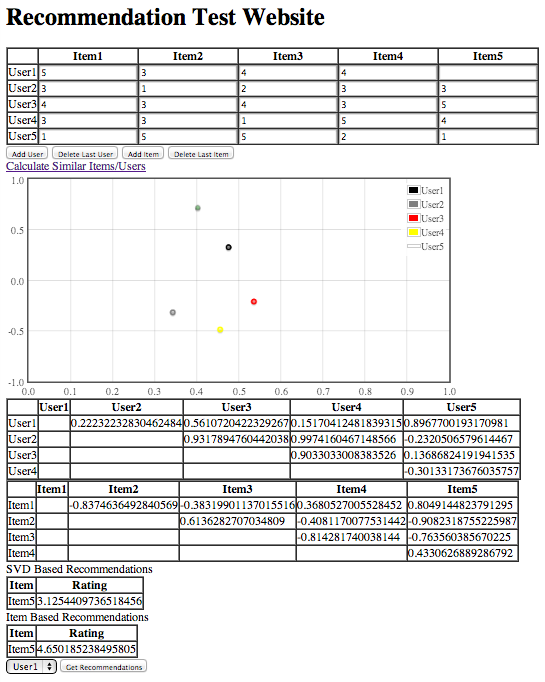
\includegraphics[width=0.75\textwidth]{image/recommendationGui.png}
  \caption{The Graphical User Interface for The Recommendation Process}
  \label{pic:recommendationGui}
\end{figure}

\section{Architecture}
The system uses a service oriented architecture. 
Thus, the main components of the system namely the tagging process, the rating system and the different recommendation techniques are encapsulated in different services.
One advantage of that architectural choice is that the system can be spread on different servers.
This does not only open the possibility to run services that have high hardware requirements on different servers but also enables the choice to duplicate services.
The duplication of services can improve service downtimes and can decrease service respond times if the service is under high load.
A disadvantage of a service oriented architecture is that it is more complex to debug system errors because each service must be debugged on its own as well as the network communication between those services.
However one requirement for this system is that the single system components should be usable separately.
With a service oriented architecture each service can be used individually over a network communication.
The network communication protocol that is necessary for communicating with the services is the HTTP protocol which is explained in subsection 3.1.3.
The next sections describe the single services and the methods that they provide.



% \tikzstyle{decision} = [diamond, draw, fill=blue!20, 
%     text width=4.5em, text badly centered, node distance=3cm, inner sep=0pt]
% \tikzstyle{block} = [rectangle, draw, fill=blue!20, 
%     text width=5em, text centered, rounded corners, minimum height=4em]
% \tikzstyle{line} = [draw, -latex']
% \tikzstyle{cloud} = [text width = 7.5em, text badly centered, draw, ellipse,fill=red!20, node distance=4cm,
%     minimum height=2em]
%     
% \begin{figure}[h]
% \begin{tikzpicture}[node distance = 2cm, auto]
%     % Place nodes
%     \node [cloud] (webservice) {Webservice};
%     \node [cloud, right of=webservice] (recommendation) {Recommendation Service};
%     \node [cloud, above right of=recommendation] (item) {Item-Based Recommendation Service};
%     \node [cloud, below right of=recommendation] (svd) {SVD-Based Recommendation Service};
%     \node [cloud, below of=recommendation] (tag) {Tagging Service};
%     \node [cloud, below of=tag] (rating) {Rating Service};
%     \node [cloud, right of=tag] (stw) {Query STW Service};
% %   \node [block] (init) {initialize model};
% %   \node [cloud, left of=init] (expert) {expert};
% %   \node [cloud, right of=init] (system) {system};
% %   \node [block, below of=init] (identify) {identify candidate models};
% %   \node [block, below of=identify] (evaluate) {evaluate candidate models};
% %   \node [block, left of=evaluate, node distance=3cm] (update) {update model};
% %   \node [decision, below of=evaluate] (decide) {is best candidate better?};
% %   \node [block, below of=decide, node distance=3cm] (stop) {stop};
%     % Draw edges
% %   \path [line] (init) -- (identify);
% %   \path [line] (identify) -- (evaluate);
% %   \path [line] (evaluate) -- (decide);
% %   \path [line] (decide) -| node [near start] {yes} (update);
% %   \path [line] (update) |- (identify);
% %   \path [line] (decide) -- node {no}(stop);
% %   \path [line,dashed] (expert) -- (init);
% %   \path [line,dashed] (system) -- (init);
% %   \path [line,dashed] (system) |- (evaluate);
%     \path [line] (webservice) -- (recommendation);
%     \path [line] (recommendation) |- (item);
%     \path [line] (recommendation) |- (svd);
%     \path [line] (webservice) |- (tag);
%     \path [line] (webservice) |- (rating);
%   \end{tikzpicture}
%   \caption{The Service Architecture of the system}
%   \label{serviceArchitecture}
% \end{figure}


%Service oriented architecture why?
%communication diagram
%explain diagram
\section{Services}
The individual parts of the system are separated into different services. 
Each service inherits from the implemented HttpServer.
This HttpServer handles the decomposing of the HTTP request, provides simple HTTP routing and creates the HTTP responses for the network communication.
Thus the services implement the service specific logic and provide methods for accessing this logic.
These methods are accessible for the router that is inherited by the HttpServer and provide a HTTP path for each method in form of a string.
Consequently the services are accessible on their specific port with HTTP Post and HTTP Get requests that correspond to the HTTP path.
\subsection{RecommendationService}
  The recommendation service controls the item based service and the svd based service.
  Therefore the single recommendation techniques can be regulated by editing the recommendation service. 
  This opens the possibility to use different recommendation approaches without much programming effort.
  \begin{table}[H]
  \begin{center}
    \begin{tabular}{| l | l | l |}
       %&Low Scroll Time and Low Time Spend & Low Scroll Time and Medium Time Spend & Item3 & Item4 & Item5 \\ 
      \hline
      \multicolumn{3}{|c|}{RecommendationService } \\ 
      \hline \hline
      Standard Port & \multicolumn{1}{l}{13000} &\\ 
      \hline \hline
      Get Methods & Parameter: Type & Return Value\\ \hline
      /calculateSimilarities & - & \\ \hline
      \multirow{2}{*}{/calculateUserPrediction} & user id: Integer & List (user, rating)\\
      & item id: Integer &\\ %\hline
      %/calculateUserPredictionsItemBased & user id: Integer & \\ \hline
      %/calculateUserPredictionsSvdBased & user id: Integer & \\ 
      \hline \hline
      Post Methods & Parameter: Type & \\ \hline
      \multirow{2}{*}{/generateRecommendations} & user id: Integer & List (user, rating)\\
      & amount: Integer & \\ \hline
    \end{tabular} 
  \end{center}
  \caption{RecommendationService}
  \label{table:recommService}
\end{table}
  The /calculateSimilatities method starts the item similarity calculation of the ItemBasedService.
  After the calculation finishes the RecommendationService starts the svd based similar user calculation of the SVDBasedService.
  These similarity values are stored in the database by the individual service for future rating predictions.
  The /calculateUserPredictions method takes a user id and an item id as parameters.
  If the item id is empty, the prediction for all items are calculated as long as enough similar item ratings exist.
  The final prediction calculation is handled by the SVDBasedService. 
  The /generateRecommendations method takes a user id, an amount of predictions that should be returned and a list of tags as parameters.
  This method forwards the parameters to the SVDBasedService and returns the list of item rating pairs to the client that send the request.



\subsection{ItemBasedService}
%der item based service ist verantwortlich fuer die item based recommendation berechnungen dh er berechnet die item similarities und kann 
  The ItemBasedService is a service that is responsible for calculating the item similarities and to predict user ratings to decrease the sparsity of the user-item table.
  It is the implemented item based recommendation concept and therefore can be used as a part of the complete recommendation concept that is introduced in this thesis.
  But at the same time it is a full functional recommendation system on its own.
  In the evaluation chapter (section 4.3) the ItemBasedService is used as a standalone recommendation system and the results are compared with the complete recommendation concept.
  \begin{table}[H]
  \begin{center}
    \begin{tabular}{| l | l | l |}
       %&Low Scroll Time and Low Time Spend & Low Scroll Time and Medium Time Spend & Item3 & Item4 & Item5 \\ 
      \hline
      \multicolumn{3}{|c|}{ItemBasedService } \\ 
      \hline \hline
      Standard Port & \multicolumn{1}{l}{13100} &\\ 
      \hline \hline
      Get Methods & Parameter: Type & Return Value\\ \hline
      /calculateSimilarItems & - & - \\ \hline
      \multirow{2}{*}{/calculateUserPrediction} & user id: Integer & List (user, rating)\\
      & item id: Integer & \\ 
      \hline \hline
      Post Methods & Parameter: Type & \\ \hline
      - & - & -\\ \hline
    \end{tabular} 
  \end{center}
  \caption{ItemBasedService}
\end{table}

  The /calculateSimilarItems method calculates the similarity between all items.
  The idea behind the similarity calculation is that the algorithm only considers to calculate the item similarity of items if they are rated together with other items by the same user.
  \begin{algorithm}
    \caption{Item Similarity Calculation}\label{alg:itemSim}
    \begin{algorithmic}[1]
      \Procedure{ItemSimilarity}{}
      \State items $\gets$ load all items
      \State seenTogether $\gets$ empty Set of item tupel
      \For{each $item_1$ in items}
        \State newItems $\gets$ empty Set of items
        \For{each user that rated $item_1$}
          \For{each $item_2$ that is rated by user}
            \If{$item_2 \neq item_1$ and seenTogether does not contain $(item_2, item_1)$} 
              \State add $(item_2, item_1)$ to seenTogether
              \State add $item_2$ to newItems
            \EndIf
          \EndFor
        \EndFor
        \State calculate similarities for $item_1$ and all items from newItems
      \EndFor

      \EndProcedure
    \end{algorithmic}
  \end{algorithm}
  The algorithm~\ref{alg:itemSim} is based on the work of \citet{amazon2003}.
  Let N be the number of items in the system and M be the number of users who rated that item.
  Then as \citet{amazon2003} stated the worst case runtime of algorithm~\ref{alg:itemSim} is $O(N^2M)$ but due to the reason that most rating tables are very sparse the runtime on a productive system is closer to $O(NM)$.
  The /calculateUserPrediction method takes a user id and an item id as parameters.
  It calculates the rating prediction for the user-item pair and returns it as a list with one element.
  If the item id is empty it calculates the user predictions for all unrated items for the specific user and returns it as a list.
  %similarity calculation where too slow on own implementation for that reason a library is used.

\subsection{SVDBasedService}
  The SVDBasedService implements the concept of the singular value decomposition based recommendation system.
  This concept states that a user-item matrix can be decomposed into three matrices.
  One of these matrices has the property that the columns of this matrix respond to the user interest of the original user-item matrix.
  With these columns the similarity between the users is calculated and with the user similarities the recommendations are generated.
  The whole concept of the singular value decomposition based recommendation is explained in more detail in subsection 2.4.2.
  The SVDBasedService is responsible for computing the recommendations after the item based service has decreased the sparsity of the rating table.
  However this service can be used as a stand-alone recommendation system which is evaluated and compared with the complete recommendation system in section 4.3.

  \begin{table}[H]
  \begin{center}
    \begin{tabular}{| l | l | l |}
       %&Low Scroll Time and Low Time Spend & Low Scroll Time and Medium Time Spend & Item3 & Item4 & Item5 \\ 
      \hline
      \multicolumn{3}{|c|}{SVDBasedService } \\ 
      \hline \hline
      Standard Port & \multicolumn{1}{l}{13200} &\\ 
      \hline \hline
      Get Methods & Parameter: Type & Return Value\\ \hline
      /calculateSimilarUsers & - & - \\ \hline
      \multirow{2}{*}{/calculateUserPrediction} & user id: Integer & List (user, rating)\\
      & item id: Integer & \\ 
      \hline \hline
      Post Methods & Parameter: Type & Return Value \\ \hline
      \multirow{2}{*}{/generateRecommendations} & user id: Integer & List (itemTitle, url, rating)\\
      & amount: Integer & \\
      & tags: List[String] & \\ \hline
    \end{tabular} 
  \end{center}
  \caption{SVDBasedService}
\end{table}

  The /calculateSimilarUsers method executes the calculation of the similar user values.
  This process is split into four steps.
  At first the user-item matrix is created out of the rating table.
  After that the method computes the singular value decomposition of the matrix.
  For this task the \emph{Apache commons-math} library is used.
  This library is a general math library with strong linear algebra algorithms developed and maintained by \emph{The Apache Software Foundation}.
  The third step is the approximation of the U matrix that is one of the resulting matrices from the singular value decomposition.
  Finally the similar users are generated by calculating the cosine similarity between all columns of the U matrix.
  This method does not have a return value. 
  All similar user values are stored in the database for future calculations.
  The /calculateUserPrediction method calculates a prediction for the specified user-item pair.
  If no item is specified the method calculates a prediction for all items that are not rated by the specified user.
  For this process the system generates a list of the most similar users $U_{sim}$.
  With these similar users it generates a list of items that these users rated but are unknown to the current user.
  For each item that is in the unknown item list the system calculates the prediction for the user-item pair as described in subsection 2.4.2.
  These predictions are returned as a list of user-item tupel.
  The /generateRecommendations method calculates the item recommendations for the current user.
  This user is the first parameter that is passed to the function.
  If the user is unknown because he is not logged in, a value of zero is passed.
  This zero user is the default user that has ratings for the most popular items.
  The second parameter specifies the amount of recommendations that the system should return.
  The third parameter that is passed to the service inside the request body as a post parameter is a string that represents a list of tags.
  The recommendations that the system generates correlate with these tags.
  The whole recommendation process is split into four steps.
  At first the tags are converted into the corresponding descriptor from the \emph{STW Standard Thesaurus Economics}(STW). 
  Afterwards the system generates a list of the most similar users for the current user.
  For each of these similar users a list is generated that contains the top rated items from this user that are unknown to the current user.
  Besides, the top rated items match the tags that are specified at the beginning of the request.
  Finally, for each of these items the rating prediction for the current user is calculated.
  The items with the highest rating predictions are used as recommendations.


\subsection{TaggingService}
  The TaggingService is the implementation of the tagging concept.
  This concept describes the process of finding the right tags for a text.
  For this process the system creates a deterministic Levenshtein automata for each word in a text.
  Every one of these deterministic Levenshtein automata reads the complete (STW).
  If a word from the STW ends in a final state the word is used as a tag for the text.
  More details about the tagging concept can be found in section 2.3.
  \begin{table}[H]
  \begin{center}
    \begin{tabular}{| l | l | l |}
       %&Low Scroll Time and Low Time Spend & Low Scroll Time and Medium Time Spend & Item3 & Item4 & Item5 \\ 
      \hline
      \multicolumn{3}{|c|}{TaggingService } \\ 
      \hline \hline
      Standard Port & \multicolumn{1}{l}{11000} &\\ 
      \hline \hline
      Get Methods & Parameter: Type & Return Value\\ \hline
      - & - & - \\ 
      \hline \hline
      Post Methods & Parameter: Type & \\ \hline
      /tagText & text: String & list of tags\\ \hline
      /descriptorsForText & text: String & list of STW descriptors\\ \hline
      /tagsForDescriptors & descriptors: List[String] & list of tags\\ \hline
      /descriptorsForTags & tags: List[String] & list of STW descriptors \\ \hline
    \end{tabular} 
  \end{center}
  \caption{TaggingService}
\end{table}

  The /tagText method takes a text as parameter. 
  The single words of the text are extracted into a list.
  For each word in this list a deterministic Levenshtein automaton is generated.
  For this process the service creates a finite automaton for each word with a specific degree.
  A degree states the maximum allowed Levenshtein distance between the word for which the automaton is generated and the word that the automaton can read.
  This degree depends on the word size.
  For a word with more than five letters a degree of three is used.
  For a word with between three and five letters a degree of 1 is used.
  Words with three or less letters are only used for direct matches.
  The states are written as tupel of the form (c, d).
  Thereby c denotes the current position in the word and d denotes the current Levenshtein distance between the prefix of the original word and the word that the automaton reads.
  For each letter in a word W with a length of n four transitions are created if the Levenshtein distance of the current state is smaller than n.
  These four transitions represent reading a correct letter, deleting a letter, inserting a letter and substituting a letter.
  The last states that are reached through the last letter do not get any transitions by this process.
  Consequently the next step is to insert the missing insertion transitions for these last states where the current position in the word is the size of the word.
  These insertions are needed because the word that is read might be longer than the original word and therefore letters must be added to the original word up to the maximum degree.
  The last step for creating this finite automaton is to mark all of the last states in which the current position in the word is the size of the word as final states.
  This finite Levenshtein automaton is transformed into a deterministic finite Levenshtein automaton. 
  This transformation process replaces every deletion transition which represents an $\epsilon$ transition by one or more new transitions.
  These new transitions start at the beginning of the $\epsilon$ transition and end at a destination of a transition that starts at the end of the $\epsilon$ transition.
  This operation has to be performed due to the fact that $\epsilon$ transitions are not allowed in deterministic automata.
  Furthermore the substitution and insertion transitions are transformed in the way that they only accept labels that are not used by any other transition from the current source.
  This process yields a deterministic Levenshtein automaton.
  Finally, all words from the STW are loaded and read into the deterministic Levenshtein automaton.
  Each word that ends in a final state is added to the list of tags that is returned to the caller.
  The /descriptorsForText method generates a list of labels for a text.
  This method is implemented the same way as the /tagText method.
  The only difference is that it converts the words which end in a final state to their corresponding STW descriptors before returning them.
  The /tagsForDescriptors method takes a list of STW descriptors as a parameter and returns the corresponding list of tags.
  For this process each preferred label is read from the triple store by its descriptors.
  The triple store contains the STW.
  The /descriptorsForTags method takes a list of tags as a parameter and returns a list of STW descriptors.
  This method loads the descriptors from the triple store that corresponds to the tags that were passed as a parameter.

  \subsection{QuerySTWService}
  The QuerySTWService is the interface between the services and the triple store.
  It provides methods for sending data to the triple store and processes the data before responding to the requests.
  This service encapsulates the triple store communication.
  Hence, it enables an integration into existing systems that use different triple store technologies by replacing only the provided methods of this service.

  \begin{table}[H]
  \begin{center}
    \begin{tabular}{| l | l | l |}
      \hline
      \multicolumn{3}{|c|}{QuerySTWService } \\ 
      \hline \hline
      Standard Port & \multicolumn{1}{l}{11500} &\\ 
      \hline \hline
      Get Methods & Parameter: Type & Return Value\\ \hline
      /descriptor & preferred label: String & descriptor \\ 
      \hline \hline
      Post Methods & Parameter: Type & Return Value\\ \hline
      /runQuery & query: String & - \\ \hline
      /descriptorsForTags & tags: List[String] & list of descriptors \\ \hline
    \end{tabular} 
  \end{center}
  \caption{QuerySTWService}
\end{table}

  The /descriptor method takes a word from the STW as a parameter and returns the descriptor of the preferred label.
  Another method that the service provides is the /runQuery method.
  This method takes a query that should be executed on the triple store as a parameter and returns the response from the triple store.
  The last method that this service provides is the /descriptorsForTags method.
  This method takes a list of tags as a parameter and returns the corresponding list of descriptors.


\subsection{RatingService}
  The RatingService is responsible for calculating and creating the user ratings for the items.
  This contains the creation process of new users and items.
  Besides the service starts the asynchronous tagging process if a new item is created and adds the tags to the items if it finishes.

%load javascript add user id item id to the page as js
%if item is unknown return javascript that reads the question and returns it to the rating service this service sends it to the tagging service
%with the tagging information it creates a new item
  \begin{table}[H]
  \begin{center}
    \begin{tabular}{| l | l | l |}
      \hline
      \multicolumn{3}{|c|}{RatingService } \\ 
      \hline \hline
      Standard Port & \multicolumn{1}{l}{12000} &\\ 
      \hline \hline
      Get Methods & Parameter: Type & Return Value\\ \hline
      - & - & - \\ 
      \hline \hline
      Post Methods & Parameter: Type & Return Value\\ \hline
      \multirow{5}{*}{/currentItem} & user id: Integer & - \\
      & item id: Integer &  \\
      & item title: String &  \\
      & item text: String &  \\ 
      & item url: String &  \\ \hline
      \multirow{4}{*}{/calculateRating} & user id: Integer & -\\
      & item id: Integer &  \\
      & time spend: Double &  \\
      & time scroll: Double &  \\
      & user interaction: Boolean &  \\ \hline
    \end{tabular} 
  \end{center}
  \caption{RatingService}
\end{table}

  The /currentItem method is called every time a user visits an item-page by a JavaScript code that is included in the item-page.
  This JavaScript code sends the item id, the item title, the item text and the user id to the \emph{WebService} which forwards these data to the rating service.
  This WebService is introduced in the following subsection.
  The /currentItem method creates a new item if the current item does not exist.
  In addition, it sends the item text to the TaggingService to get the tags for this item. 
  Moreover, it creates a new user if the current user is unknown to the system.
  The same JavaScript code is responsible for sending every two seconds a request to the WebService.
  This request includes the current time that the user has stayed on the page (CT), the time a user has scrolled on the page (ST), the user id and the item id.
  Then the WebService forwards the data to the /calculateRating method.
  The design choice of sending the data periodically every two seconds to the server has been made for the reason that sending the complete data set if the user leaves the website is not reliable enough and can lead to the loss of these rating information.
  After the /calculateRating method receives the CT and ST times it adds these times to the previously received times or creates a new table entry with the times for that user.
  With these new times the method calculates the new rating for that item and stores it in the database.

\subsection{WebService}
  The WebService is the interface for external clients which are usually web browser that visit item pages or the developed recommendation test page.
  This service forwards external enquiries and processes data before it sends the data back to the client.
  Furthermore it provides an interface for accessing the database objects for the \emph{backbone.js} application that represents the \emph{recommendation test website} as well as an interface for accessing static files like JavaScript and HTML files.

  \begin{table}[H]
  \begin{center}
    \begin{tabular}{| l | l | l |}
      \hline
      \multicolumn{3}{|c|}{WebService } \\ 
      \hline \hline
      Standard Port & \multicolumn{1}{l}{10000} &\\ 
      \hline \hline
      Get Methods & Parameter: Type & Return Value\\ \hline
      / & - & index.html \\ \hline
      /tagger & - & tagger.html \\ \hline
      \multirow{2}{*}{/data} & type: String & model\\
      & id: Integer &  \\ \hline
      /file & path: String & document\\ \hline
      \multirow{2}{*}{/calculate} & type: String & result\\
      & id: Integer &  \\ \hline
      \multirow{2}{*}{/recommendation} & user id: Integer & JavaScript code\\
      & amount: Integer &  \\ 
      & tags: List[String] &  \\ 
      \hline \hline
      Post Methods & Parameter: Type & Return Value\\ \hline
      /data & model: Object & - \\ \hline
      /rating & * & - \\ \hline

    \end{tabular} 
  \end{center}
  \caption{WebService}
\end{table}

  The / and the /tagger methods are both returning specific static HTML files from the file system.
  These methods should be deactivated for the production mode.
  The / method returns the index.html file which is the main page for the recommendation test website.
  Additionally the /tagger method returns the tagger.html website which is a website for testing the TaggingService.
  The /calculate method forwards the calculation requests that can be specified by a provided type parameter to the RecommendationService.
  For the provided type parameter the client can use \emph{similarities}, \emph{recommendations} and \emph{recommendationsItemBased}.
  If a client sends a request for similarities to the WebService, the service starts the calculations for similar users and items on the RecommendationService.
  A user id is not necessary for this request.
  By sending the \emph{recommendations} type together with a user id to the /calculate method the service sends a request to the RecommendationService for calculating all predictions for the items that the user has not yet rated.
  The \emph{recommendationsItemBased} type has the same effect as the \emph{recommendations} type.
  The only difference is that the predictions are calculated with the item based approach instead of the standard SVD based approach.
  The /recommendation method is usually called by an HTML website that expects a JavaScript code that is embedded into the page.
  The method takes a user id, the amount of recommendations and a list of tags as a parameter.
  These data is forwarded to the recommendation system.
  However, the returned list of item recommendations is transformed into a HTML link for each recommendation.
  These HTML links are embedded into a JavaScript code that is returned by the service.
  This JavaScript code inserts all item links into a specified HTML Div container.
  There are three /data methods that are interfaces for reading, creating, updating and deleting entries in the database.
  These interfaces are necessary for the backbone.js framework that is used for building the recommendation test website.
  The first method that is called via a post request updates existing entries in the database or creates new entries for the provided parameter.  
  The second method which is called via a get request reads data from the database.
  The type that is provided as a parameter represents the database table from where the data should be read.
  If an id is provided as a parameter, the service returns the specific entry.
  Otherwise the service returns all entries from the database table.
  The third method is accessible via a HTTP delete method and must provide a type and an id.
  The specific entry with the corresponding id from the database table that is specified by the type is deleted by the service.
  The /rating method forwards all requests to the RatingService.

  \section{Service Relations}
  This section explains the relations between the services.
  The whole system can be separated into three use cases.
  The first use case is the situation when a user visits an item page.
  This situation is illustrated by a sequence diagram in figure~\ref{seq:userVisits}.
  When a user visits a website that recommends items to users it belongs to the second use case.
  The sequence diagram figure~\ref{seq:userVisits} describes this situation.
  The third use case is the situation in which the system starts the calculation of the user and item similarities.
  It is presented in the sequence diagram in figure~\ref{seq:calc}.

  \subsection{User Visits Item Page}
  The use case that occurs if a user visits an item page is illustrated in the sequence diagram in figure~\ref{seq:rec}.
  The web browser that executes the JavaScript code that is embedded in each item page sends the current information about the item and the user to the WebService.
  However, the web browser does not expect a response.
  The WebService checks if the data is complete and forwards the request to the RatingService.
  The sequence diagram from figure~\ref{seq:rec} represents the situation when the item and the user are unknown to the system.
  Therefore the RatingService creates a new item and a new user.
  Besides, the RatingService sends the text of the item together with its title to the TaggingService.
  The TaggingService creates a Levenshtein distance automaton for each word in the text and requests all words that are included in the STW from the QuerySTWService.
  The words from the STW are tested with the Levenshtein automata.
  Each word that ends in a final state is returned in a list of tags.
  Finally, the returned tags are added to the newly created item.

  Additionally, the web browser sends periodically the time that the user spends on the website together with the time that the user scrolls on the website to the WebService.
  This data is needed to calculate the implicit user rating for the item.
  The WebService forwards the request to the RatingService which updates the times in the database and calculates the new rating.



\begin{figure}[h]
  \centering

  \begin{sequencediagram}
    \newthread{wb}{Web Browser}
    \newinst{ws}{WebService}
    \newinst{rs}{RatingService}
    \newinst{ts}{TaggingService}
    \newinst{qs}{QuerySTWS.}

    \begin{call}{wb}{Visits Item Page.}{ws}{}
      \begin{call}{ws}{currentItem}{rs}{}
        \begin{call}{rs}{tagText}{ts}{tags}
          \begin{callself}{rs}{createItem}{}
          \end{callself}
          \begin{callself}{rs}{createUser}{}
          \end{callself}
          \begin{call}{ts}{runQuery}{qs}{labels}
          \end{call}
          \begin{callself}{ts}{Levenshtein}{tags}
          \end{callself}
        \end{call}
      \end{call}
    \end{call}
    \begin{call}{wb}{calcRating}{ws}{}
      \begin{call}{ws}{calcRating}{rs}{}
        \begin{callself}{rs}{calcRating}{save rating}
        \end{callself}
      \end{call}
    \end{call}
  \end{sequencediagram}

  \caption{User Visits Item Page Sequence Diagram}
  \label{seq:userVisits}
\end{figure}



  \subsection{User Visits Recommendation Website}
  This subsection describes the network communication between the services if a user visits a website that recommends items.
  The sequence diagram in figure~\ref{seq:rec} represents the network communication between the involved services.
  The website that has to display the recommendations communicates with the system by including a JavaScript file from the system.
  The path for this JavaScript file includes optional parameters namely the user id, the amount of recommendations and tags.
  If the current user is not registered, the system uses a standard user for generating recommendations.
  The tags are used for filtering the items so that the recommended items match the subject of the website.
  The web browser requests the JavaScript file from the WebService, which is basically the interface for external clients for the internal services.
  Thus, the WebService forwards the request to the RecommendationService.
  This RecommendationService requests the recommendation calculation on the currently activated recommendation system.
  The latter is the SVDBasedService in the sequence diagram. 
  Another option would be the ItemBasedService.
  The SVDBasedService passes the tags to the TaggingService which translates them to the corresponding descriptors by communicating with the triple store via the QuerySTWService.
  The latter returns the descriptors to the TaggingService which passes the returned descriptor list on to the SVDBasedService.
  This SVDBasedService generates the item list which includes the items with the highest rating prediction for the current user that match the subject of the tags.
  This item list is returned to the RecommendationService.
  The RecommendationService hands the item list to the WebService.
  The WebService creates html links for each of the items in the list and embeds these links into the requested JavaScript file.
  The web browser executes the JavaScript file and, thus, inserts the recommended item links into the website.


%The http get and post request are the standard requests that are used by web
%browsers to send data.
%answer by http request respond
%explain http
\footnotesize
\begin{figure}[h]
  \centering

  \begin{sequencediagram}
    \newthread{wb}{Web Browser}
    \newinst{ws}{WebService}
    \newinst{rs}{Recom.Service}
    \newinst{ss}{SVDB.Service}
    \newinst{ts}{TaggingService}
    \newinst{qs}{QuerySTWS.}

    \begin{call}{wb}{gen.Recomm.}{ws}{Javascript}
      \begin{call}{ws}{gen.Recomm.}{rs}{Predictions}
        \begin{call}{rs}{gen.Recomm.}{ss}{Predictions}
          \begin{call}{ss}{descriptorsTags}{ts}{descriptors}
            \begin{call}{ts}{runQuery}{qs}{descriptors}
            \end{call}
          \end{call}
          \begin{callself}{ss}{calculateRecommendation}{}
          \end{callself}
        \end{call}
      \end{call}
      \begin{callself}{ws}{convert Prediction to JS}{}
      \end{callself}
    \end{call}
  \end{sequencediagram}
  \caption{Embedded Recommendations Sequence Diagram}
  \label{seq:rec}
\end{figure}
\normalsize

  \subsection{System Calculates Similarities}

  The system requests the calculation of similar user and similar item values from the RecommendationService.
  The RecommendationService calculates the average user ratings and the average item ratings.
  Additionally, the service requests the calculation of the user similarities by the SVDBasedService and the calculation of the item similarities by the ItemBasedService. 
  Each of these services stores the calculated values in the database.
  This should occur periodically every 24 hours to once a week depending on the frequency that the item catalog changes and the frequency that new user ratings are generated.



\begin{figure}[h]
  \centering

  \begin{sequencediagram}
    \newthread{system}{System}
    \newinst{rs}{RecommendationService}
    \newinst{ss}{SVDBasedService}
    \newinst{is}{ItemBasedService}

    \begin{call}{system}{startCalculation}{rs}{}
      \begin{callself}{rs}{Calc. Avg. User rating}{}
      \end{callself}
      \begin{callself}{rs}{Calc. Avg. Item rating}{}
      \end{callself}
      \begin{call}{rs}{Calc. Sim. Users}{ss}{}
      \end{call}
      \begin{call}{rs}{Calc. Sim. Items}{is}{}
      \end{call}
    \end{call}
  \end{sequencediagram}
  \caption{System Calculates Similarities Sequence Diagram}
  \label{seq:calc}
\end{figure}



\chapter{Evaluation}
\label{chapter:evaluation}
In this chapter the different concepts that are introduced in this thesis are evaluated.
The first section deals with the rating concept and evaluates the quality of the ratings that are generated for the individual user interaction on a web page.
The second section evaluates the time and the quality of the tagging concept by applying the tagging algorithm on texts with different word counts.
Moreover the tags that are returned by the algorithm are compared with the tags that should have been returned by the algorithm.
Finally different recommendation techniques are compared by the run time and the quality of their predictions.

\section{Rating}
The evaluation for the rating system refers to the rating concept from subsection 2.2.5.
This concept is build upon the researches from \citet{claypool2001} who evaluated different user interactions and compared those with explicit user ratings.
The two user interactions that performed the best with an accuracy of approximately 70\% to the explicit user ratings are the time a user spends on a website and the time a user scrolls.
Each of these measured times of the user interactions are split into segments depending on the truncated mean time of all user times, yielding a scale that enables the system to calculate ratings based on the user interactions.
Based on this scale the ratings are calculated separately and are combined to the complete rating by calculating the average of both ratings.
This complete rating is evaluated with the research data from \citet{claypool2001} in this section.
For the rating evaluation one question page of the \emph{askbot} question and answer website is used.
This question page has a truncated mean time for the time a user spends on the website and another truncated mean time for the time a user scrolls on the website.
For these truncated mean times the average times from all user ratings of the field test from \citet{claypool2001} are used.
These average times are 5.339 seconds for the time a user scrolls and 20.763 seconds for the time a user spends on a website.
Finally, users who visit the website are simulated.
Those users are interacting with the website according to the times of \citet{claypool2001} field experiment.
Therefore, the ratings that the simulated users generate can be compared to the data from the team of \citet{claypool2001}.

\begin{table}[H]
  \begin{center}
    \begin{tabular}{| l | l | l | l | l | }
      \hline
      \multicolumn{5}{|c|}{Rating Algorithm Evaluation} \\ 
      \hline \hline
      Scroll Time & Scroll Rating & Time Spend & Time Rating & Complete Rating \\ \hline
      3.559 & 1 & 14.012 & 1 & 1 \\ \hline
      3.249 & 1 & 21.603 & 3 & 2 \\ \hline
      3.355 & 1 & 25.497 & 4 & 3 \\ \hline
      5.077 & 3 & 13.414 & 1 & 2 \\ \hline
      5.342 & 3 & 21.217 & 3 & 3 \\ \hline
      5.287 & 3 & 26.797 & 4 & 4 \\ \hline
      7.374 & 5 & 12.113 & 1 & 3 \\ \hline
      7.504 & 5 & 20.917 & 3 & 4 \\ \hline
      7.431 & 5 & 24.797 & 4 & 5 \\ \hline
    \end{tabular} 
  \end{center}
  \caption{Rating Algorithm Evaluation}
  \label{table:ratingEv}
\end{table}

Table~\ref{table:ratingEv} represents the results of the rating algorithm evaluation.
  The \emph{Scroll Time} represents the time that a user scrolls on the page and the \emph{Scroll Rating} represents the rating that results out of that scrolling behaviour.
  Additionally, the \emph{Time Spend} represents the time that a user spends on the web page and the \emph{Time Rating} represents the rating that the system generates for that behaviour.
  The complete rating is the implicit rating that the system uses as the rating of that user for the specific item.
  These complete ratings are integer values and are therefore rounded.
  The values of the Scroll Time nearly match the average times that were found as rating indicators in the field experiment from \citet{claypool2001}.
  These average times that a user scrolls on a web page and rates the site with an explicit rating are 3.485 seconds for an explicit rating of 1, 4.079 seconds for an explicit rating of 2, 5.267 seconds for an explicit rating of 3, 6.444 seconds for an explicit rating of 4 and 7427 seconds for an explicit rating of 5.
  All generated Scroll Ratings reflect the expected ratings from the field test of \citet{claypool2001}.
  The same is true for the generated Time Ratings.
  The Time Spend values nearly match the average times for the specific ratings from the \citet{claypool2001} field experiment.
  These average times are 13.414 for a rating of 1, 18.017 for a rating of 2, 21.217 for a rating of 3, 24.372 for a rating of 4 and 26.797 for a rating of 5.
  However, the rating of five could not be achieved by spending time on the web page because this rating is only attainable by performing a pre defined user interaction such as clicking on a specific button.
  All other Time Ratings reflect the expected ratings from the field experiment of \citet{claypool2001}.
  The \emph{Complete Rating} which is introduced in this thesis correlates with the combined user interest of the Scroll Rating and the Time Rating and therefore represents the expected result.
  Moreover, the complete rating is derived from the data of \citet{claypool2001} and it would have been desirable to conduct a field experiment but unfortunately due to the lack of time this was not possible and should be considered for future works.


%%daher wurde getestet ob unterschiedliche surfverhalten unterschiedliche ratings hervorbringen. und ob diese mit den in chapter 2 section 2.2 subsubsection 2.2.5 vorgestellten theorien uebereinstimmen
\section{Tagging}
This section evaluates the tagging process that was introduced in subsection 2.3.2.
The concept behind the tagging process is to create a \emph{Levenshtein automaton} for every word in an item and read each word from the \emph{STW Standard Thesaurus Economics}(STW) into the automaton.
If the word ends in a final state it is used as a tag for the item.
Such a Levenshtein automaton is a deterministic finite automata that can decide in linear time if a word has a Levenshtein distance smaller than a desired $n\in\mathbb{N}$.
Four different texts are created for the evaluation process. 
In each of these four texts 70\% of the words are from a placeholder text that is called \emph{Lorem ipsum}.
The Lorem ipsum text is according to \cite{wiki:lorem} typically based on a Latin text from Cicero with words altered, added and removed.
Thus it is not a proper Latin text any more.
These words are chosen based on the fact that they do not match with the words from the STW.
Consequently, they do not create false matches during the evaluation process.
The other 30\% of the words in the evaluation texts are from the STW.
However, not all of the words are in the same form as they are found in the STW.
Therefore, the tagging algorithm has to match the words from the item with the correct words from the STW.
After each test the matched words are compared to the words that should have matched.
Besides, the time that the algorithm needed for creating all Levenshtein automata and the total time in seconds is evaluated.
The results of this evaluation can be seen in table~\ref{table:taggingEv}.
The computer that is used for testing this tagging algorithm is a \emph{Macbook Air} with a 1.86 \emph{GHz Intel Core 2 Duo} precessor and 4 GB DDR3 memory.

\begin{table}[H]
  \begin{center}
    \begin{tabular}{| l | l | l | l | l | l |}
      \hline
      \multicolumn{6}{|c|}{Tagging Algorithm Evaluation} \\ 
      \hline \hline
      Words & STW & Non Matching & Matched Words & Levenshtein Time & Total Time \\ \hline
      1 & 1 & 0 & 2 & 0.099 & 14.481 \\ \hline
      10 & 3 & 7 & 3 & 0.2843 & 20.348 \\ \hline
      100 & 30 & 70 & 54 & 0.4751 & 79.9616\\ \hline
      1000 & 300 & 700 & 470 & 2.5606 & 777.4643\\ \hline
    \end{tabular} 
  \end{center}
  \caption{Tagging Algorithm Evaluation}
  \label{table:taggingEv}
\end{table}

  At first the word \emph{tests} is used with the tagging algorithm.
  This evaluation results two matches from the STW namely \emph{test} once for the English and once for the German language.
  The time that is needed for creating the Levenshtein automaton is approximately a tenth of a second.
  For this complicated generation process this is a good performance.
  However the total computation time is 14.481 seconds which involves the loading of the 31.682 words from the STW and the reading of all of these words into the Levenshtein automaton.

  For the second evaluation ten words are used with seven non matching words and three words from the STW.
  Two of the three words are modified. 
  Hence, they are not in the same form as they appear in the STW.
  All three of these words are matched by the tagging algorithm.
  The creation time of all Levenshtein automata is 0.2843 seconds which is approximately three times as high as the Levenshtein automaton computation time for the one word creation.
  The total computation time of 20.348 seconds is 1.5 times higher than the total computation time for the one word tagging process.

  The 100 words evaluation consist of 30 words from the STW with spelling mistakes and different forms.
  The other 70 words are non matching words from the Lorem ipsum placeholder text. 
  The algorithm returns 54 words as matches from the STW.
  These 54 words include all 30 words that were included in the original 100 words plus 24 words that are similar spelled or use the same words in English and German.
  The computation time for all 100 Levenshtein automata is 0.4751 and in total the computation needs 79.9616 seconds.

  The last tagging algorithm evaluation uses a text with 1000 words.
  This text contains 300 words from the STW with approximately 150 words in different forms or with spelling mistakes.
  The other 700 words are words from the Lorem ipsum placeholder text and, thus, are non matching.
  The algorithm returns 470 words whereby almost all of the original words were included.
  The words that did not match are the words that had more than three changes resulting from changing the singular form to its plural form and adding spelling mistakes.
  The computation time for the Levenshtein automata is five times higher than the corresponding time for the 100 word test.
  Anyhow, the total computation time is nearly ten times higher than the total time for the 100 word test.

  %fazit man sollte seine aufmerksamkeit nicht auf beschleunigung des erstellungs prozesses des levenshtein automatas legen sondern auf die korrekte auswahl der tagging base 
  A conclusion of this evaluation is that the largest part of the total time is the reading of the words from the tagging base into the Levenshtein automata and not the time that the algorithm needs to create these automata.
  Consequently, the main focus in future works should not be to improve the performance of the creation process of the Levenshtein automata but to decrease the number of words in the tagging base.

\section{Recommendation}
This section evaluates the different recommendation approaches that are explained in subsection 2.4.4.
These different approaches are the item-based recommendation, the different singular valued decomposition (SVD) based recommendations, and the approach that is described in this thesis that uses item-based predictions to decrease the sparsity of the rating table and the SVD-based approach for recommendations.
The evaluation process of the recommendation system contains two parts.
Firstly, the evaluation of the performance of the different approaches by using the wall clock time.
Secondly, the comparison of the accuracy of the different concepts.
For this task the \emph{MovieLens} database is used.
The MovieLens database includes 100.000 ratings from 943 users for 1682 movies.
This data is collected with the movielens.org website that is part of the \emph{GroupLens} research project from the University of Minnesota.
The website is a recommendation website for movies.
Each user of the website can rate movies on a scale from 1 to 5 and is afterwards presented with movies that might be interesting for him.
To compare the accuracy of the recommendation systems the \emph{Mean Absolute Error} (MAE) is used which is according to \citet{sarwar2001} most commonly used for evaluating recommendation systems.

\begin{definition}[Mean Absolute Error]
  Let $p_{i, j}$ be the predicted rating for user i and item j and let $q_{i, j}$ be the real rating for user i and item j.
  Then the following formula calculates the MAE.
  \begin{displaymath}
    MAE = \frac{\sum_{u \in U}\sum_{i \in testset_u} |rec(u, i) - r_{u,i}|}{\sum_{u \in U}|testset_u|}
  \end{displaymath}
\end{definition}

The MAE is a statistical metric that compares the calculated user-item ratings from the recommendation system with real user-item ratings. 
For this process the recommendation system is trained with a percentage p of a test rating database and afterwards the remaining 1-p percent are used to check if the recommendations are correct.
A ratio of 80\% training data and 20\% prediction data is used.

The team of \citet{Herlocker04evaluatingcollaborative} noticed that many collaborative recommendation systems in the movie domain reach a mean absolute error of up to 0.73 on a rating scale from 1 to 5.
Out of this realisation \citet{Herlocker04evaluatingcollaborative} created the hypothesis that collaborative recommendation systems which are tuned to its optimum cannot get much more accurate than a mean absolute error of 0.73.
They explain this hypothesis by reasoning that users tend to provide inconsistent ratings when they are asked to rate the same movie at different times.
Hence, an algorithm cannot be more accurate than the users rating variance for the same item.

\begin{table}
  \begin{center}
    \begin{tabular}{| l | l | l | l |}
      \hline
      \multicolumn{4}{|c|}{Recommendation System Evaluation 80.000 ratings 20.000 predictions} \\ 
      \hline \hline
      Technology & MAE & Offline Computation Time & Prediction Time \\ \hline
      Item Based & 0.83187 & 3187.69 & 4208.49\\ \hline
      SVD Concept & 0.77937 & 32471.93 & 4315.31\\ \hline
      SVD Three & 0.79545 & 469.82 & 4395.75\\ \hline
      SVD Average & 0.78622 & 507.90 & 4226.31\\ \hline
      Three & 1.03333 & 0.00 & 0.49\\ \hline
      Average & 0.82714 & 112.13 & 249.18\\ \hline
    \end{tabular} 
  \end{center}
  \caption{Recommendation System Evaluation}
  \label{table:recomEv}
\end{table}

The table~\ref{table:recomEv} represents the evaluation of the recommendation systems.
  The computer that is used for testing the different recommendation techniques is a \emph{Macbook Air} with a 1.86 \emph{GHz Intel Core 2 Duo} precessor and 4 GB DDR3 memory.
  Consequently, all computation times that are measured in this evaluation are based on this hardware system and can be faster on a productive server.
  However, the computation times can be used to compare the speed of the different recommendation systems.
  The evaluation contains three different metrics the mean absolute error, the offline computation time and the prediction time.
  The mean absolute error is, as explained before, a statistical metric that declares the average distance between the predicted user-item rating and the real user-item rating.
  The offline computation time represents the time that the system needs to generate the data that is needed for the prediction of the items.
  Hence, this computation must not be calculated for every recommendation but every 24 hours to once a week depending on the frequency that new items are added to the system and the activeness of the users in order to ensure the correctness of the user and item similarities.
  The prediction time is the time that the system needs to calculate the predictions for all 20.000 ratings.
  Therefore, this time divided by 20.000 represents approximately the time that the system needs to calculate one prediction for the recommendations that are presented to the user on a website.

  The \emph{Item Based} technology is the implementation of the item based recommendation approach that is part of the overall recommendation concept of this thesis.
  It has a mean absolute error of 0.83187 which is the second poorest mean absolute error of all tested technologies.
  This is a surprising outcome of the evaluation because it was expected that this technology would be more similar to the mean absolute error of the SVD based technologies. 
  The offline computation time in this implementation consists of finding items that were rated by the same users and calculating the adjusted cosine similarity between those items.
  The adjusted cosine similarity is a special form of the cosine similarity.
  The cosine similarity for two items is calculated by applying the dot product between the rating vectors of the items and dividing the result by the Euclidean length of the rating vectors.
  The adjusted cosine similarity uses the same computation but normalizes the ratings in the rating vectors before calculating the cosine similarity.
  This normalization consists of subtracting the average user rating from the rating to remove the individual rating behaviour of the user.
  This process is explained in more detail in subsection 2.4.2.
  The calculation of the adjusted cosine similarity between all items takes the largest part of the computation time.
  At last the item similarities are stored in the database.

  The prediction time for a user-item pair involves the finding of similar items that the user has rated and calculating the sum of the product of the similarity and the rating and dividing the result by the sum of the similarities.
  So, all in all the implemented Item Based technique has the second slowest offline calculation time and with an average distance of 0.83 between the predicted rating and the actual rating one of the poorest mean absolute errors of the implemented methods.

  The \emph{SVD Concept} technology represents the recommendation system that is introduced in this thesis.
  Therefore, it uses item based rating predictions to fill empty rating entries in the user-item rating matrix with predictions.
  The mean absolute error of this technology is the best of all implementations that were tested.
  In terms of the other SVD based implementations this can be explained by the fact that the rating matrix has the most accurate entries of all.
  However, the SVD Concept has a very high offline computation time.
  The offline computation time of this system contains the following calculations.
  At first the average user rating is calculated which is needed to remove the individual rating behaviour from the user ratings before calculating the predictions.
  Thereafter the item based cosine similarity is calculated which contains the same parts that where explained for the offline computation time of the Item Based technology.
  After that for each user the rating prediction of the missing user-item entries in the rating table is calculated which is responsible for the largest part of the total computation time.
  The computation time for each user is approximately 30 seconds and the test database consists of 943 users.
  This can be explained by the fact that each user has only rated a fraction of all items and therefore many predictions must be calculated.
  Afterwards the rating matrix is generated from the rating table.
  The entries of the matrix represent a rating for a user-item pair.
  The previously generated rating predictions are used for empty entries in the rating matrix.
  For this rating matrix a singular value decomposition is generated.
  This process decomposes the rating matrix into three matrices namely U, V and $\Sigma$.
  The matrix U has the property that each column of the matrix represents the interest of a user.
  More details to the singular value decomposition and the features of the three matrices are described in subsection 2.4.2.
  In addition, the matrix U is reduced to the two dimensional approximation to decrease the following computation time.
  This computation time is the calculation of the cosine similarity between the columns of the two dimensional approximation of the matrix U.
  These similarities are used to created the final rating predictions for the item recommendations when a user visits a website.
  Finally, the user similarities are stored in the database.

  The prediction time consists of finding similar users that rated a specific item and calculating the prediction with the similarity of the users and their ratings.
  Overall this technique has the best mean absolute error but it has the slowest offline computation time. 

  The \emph{SVD Three} technology represents a singular value based recommendation system that uses a rating of three to fill in the missing user-item ratings in the rating matrix.
  The rating of three is used because it represents the middle of the rating scale of 1 to 5 and therefore it should have the least distance between all ratings if the ratings are uniformly distributed.
  The mean absolute error of this implementation is 0.79545 which is the poorest of the SVD based approaches.
  This is expected because it generates the singular value decomposition with a rating matrix that uses static values for the missing entries.
  This matrix should have the highest difference to the matrix that would represent the real user interest and hence should generate the poorest user similarities.
  The offline computation time of this system consist mostly of the same parts as the SVD Concept.
  These parts are calculating the average user rating for each user, creating the rating matrix from the database and calculating the singular value decomposition as well as creating the approximation of the matrix U that is part of the singular value decomposition.
  Besides the offlise calculation includes the calculation of the cosine similarity between the columns of the matrix U approximation and the storing of these user similarities in the database.
  The calculations that are created during the prediction time are the same as the calculations that were used in the SVD Concept approach namely the finding of similar users that rated a specific item and the calculation of the predictions.
  This system is evaluated in order to compare the impact of the values that are used to fill in the missing ratings in the rating matrix.
  This evaluation demonstrates that the more accurate these values are the better is the quality of the predictions.
  However, the difference of the mean absolute error of this approach and the other two SVD based approaches is smaller than expected.
  Therefore, further developments that should improve the prediction accuracy should be concentrated on the prediction calculation and not on the improvement of the similarity calculations.
  Altogether this technique has the fastest offline calculation time of all tested more advanced recommendation systems and a good mean absolute error.

  The \emph{SVD Average} technology is the implementation of the SVD based approach but it uses the average item ratings to fill in the missing entries of the rating matrix.
  Therefore, it is a solution without complex calculations to create dynamic rating predictions for the missing entries in the rating matrix that mirror the overall user interest.
  The mean absolute error is 0.78622 and, thus, it has the second best mean absolute error of all tested systems.
  The offline calculation time consists of calculating the average user ratings and calculating the average item ratings as well as all other calculations that are needed in the SVD Three approach.
  The singular value decomposition works in the same manner as the one in the SVD Three approach with one difference it uses the average ratings of the items to fill the missing entries in the rating matrix.
  The prediction time of 4226.31 seconds includes the same calculations that were used for the other two SVD based approaches which are the finding of similar users that rated a specific item and the calculation of the predictions.
  Hence, it has almost the same prediction time as the other SVD based approaches that were tested in this evaluation.
  To sum this up this technique has the second best mean absolute error and moreover it has one of the fastest offline computation times of the tested more advance recommendation systems.
  Thus, this system has a fast computation time and a very good mean absolute error and for this reasons it should be used for further developments if the quality of the recommendations is more important than the computation time.

  The last two systems are added to the evaluation to compare the results of the more advanced recommendation systems with less advanced approaches.
  The \emph{Three} technique uses a rating of three for all predictions.
  The three was chosen because it represents the middle of the five point rating scale. 
  Therefore, it has the smallest mean absolute error of 1.2 of all static ratings if the user ratings are evenly distributed.
  This technique does not require any offline computations and the mean absolute error calculation consists of subtracting the real rating from three.
  This approach yields a MAE of 1.03333.
  Consequently, the ratings are less common on the outer boundaries of the rating scale which is a common user rating behaviour.
  The MAE of 1.03333 can be seen as a lower boundary.
  If any of the recommendation techniques is below this MAE, it is an indicator that the recommendation technique does not work properly. 

  The \emph{Average} technique uses the average item rating as a rating prediction.
  Thus, it is the least complex method which generates dynamical rating predictions that represent the interest of all users.
  The difference from its MAE of 0.82714 to the lower boundary of 1.03333 is 0.20619 which is a good result.
  Additionally, it has nearly the same mean absolute error as the item based approach.
  Hence, it can be concluded that the interests of the individual users from the \emph{MovieLens} database does not vary widely.
  This technique only has to calculate the average user ratings of all users for the offline computation time which is very fast.
  Besides it only needs to load one value from the database for the prediction calculation instead of calculating a prediction.
  As a result the Average technique is a good choice if the user interest of the system does not vary widely and if the system needs a fast solution.

  In conclusion the evaluation of the recommendation techniques revealed that the SVD based approach that was introduced in this thesis has the best mean absolute error of the implemented approaches.
  Anyway, it does not vary widely from the MAE of the SVD Average technique whereby the offline computation time of the SVD Concept approach is by far the slowest.
  The item based approach has a slow computation time and the MAE is nearly the same as the Average approach.
  The research team of \citet{sarwar2001} showed that this method can yield a MAE of up to 0.73 by improving the prediction calculation.
  However these improvements should have the same effect for the SVD based approaches and therefore the SVD based techniques should be the better choice for collaborative recommendation systems.
  The evaluation of the SVD Three technique indicates that SVD based recommendation systems generally result in good predictions.
  Moreover, it showed that improvements for the missing entries for the rating matrix yield improvements of the predictions but that these optimizations only improve the MAE by approximately 0.2 points.
  Therefore, future works with the goal of optimizing collaborative recommendations should concentrate on the improvement of the prediction calculations.
  Finally, the evaluation revealed that using the average user rating as a rating prediction can yield good and fast predictions if the user interest does not vary widely.
  Consequently, this can be used for calculating rating predictions as part of recommendation systems if the use case of the system does not require highly optimized recommendations.
  This evaluation should be repeated when the system is in productive usage and has collected the same amount of data that was used for this evaluation to check if the data for the specific use case of recommending questions and answers reveal the same findings as this evaluation.



\chapter{Conclusion}
%wiederhole die herausforderungen und ziele der arbeit und erklaere meine contribution to the field
%section: what have i done and how und stelle dar wie diese geloest wurden
%section: what are the main findings show links across the structure
%section: future work
%section: summary great original contribution highly significant
%verdeutliche den teil den du selbst gemach hast und stelle die ergebnisse dar
  The focus of this thesis is the development of a recommendation system for user generated content.
  These recommendations should match the user interest and the context of the website on which they are included.
  For this purpose it is important to analyze the user generated content with regard to quality and to be able to identify the subject of the content automatically.
  Hence, user interactions that can occur on a website are evaluated to be able to tell if a user might be interested in the content.
  Based on the research of \citet{claypool2001} the time a user spends on a website and the time a user scrolls on a website are chosen for generating implicit user ratings.
  These two user interactions correspond about 70\% of the time with the explicit ratings of a user.
  The times of each of these interactions are used separately for creating a scale that expresses user ratings by these times.
  The average of these two ratings is then used as the complete rating.
  This concept is evaluated with simulated user interactions.
  The result of this simulation displays that the two separate ratings agree with the findings of \citet{claypool2001}.
  Besides, the complete ratings are as expected.
  However, for this part of the thesis a field test in the future would be a good idea to adjust the formula according to the use case.
  %unterschiedliche concepte zum approximativen string matchen wurden discussed 
  %die idee des levenshtein automata wurde aufgegriffen und in das gesamt concept integriert hierfuer wurden maximale word distancen selectiert in abhaengigkeit der wortlaenge
  For the categorization of the user generated content the words of the content are matched with words from a thesaurus.
  For this task different error allowing string matching methods are evaluated. 
  The chosen concept is the \emph{Levenshtein automaton} which is a special automaton for approximate string matching.
  Based on the work of \citet{schulz2002} the algorithm for a deterministic Levenshtein automata is integrated into the overall concept.
  Besides, a concept for finding the maximum \emph{Levenshtein distance} for a word depending on its length is introduced in this thesis.
  This is important because a word with a small word size can not be handled the same way as a word with a long size.
  The smaller word need a smaller distance otherwise it would generate too many false matches.
  This word match algorithm is used to find the keywords of a text and to use them as tags.
  This enables the system to presort the content by the keywords before recommending it on a website. 
  The tagging process is evaluated by using texts with a different amount of words.
  Each of those texts has 30\% words that should match with the words in the thesaurus.
  However, most of these words are in a different form or spelling mistakes are inserted.
  So, the evaluation process checks how many words are found and how long the algorithm needs.
  In three of four tests more words were returned than the algorithm should have matched.
  This is mostly due to the fact that most words in the thesaurus are included in the German and English language and that some of those words are quite similar.
  Consequently the algorithm returns the English and the German word.
  Other false matches occurred because the thesaurus included words that were too similar and thus the algorithm returned both of these words.
  Therefore, a future optimization would be to reduce the size of the tagging base which would not just reduce the occurrence of false matches but would also decrease the time that the algorithm needs to find the tags.
  Another possible future work is to decide whether the text is in the German or English language and to use only the words from the corresponding language as a tagging base.
  In addition, different types of recommender systems are discussed.
  The conclusion of this discussion is that for the use case of recommending user generated content a collaborative recommendation system is the best approach.
  Two existing collaborative recommendation techniques are explained namely the item based technique and a recommendation technique based on singular value decomposition.
  These techniques are combined into a new recommendation concept which is introduced in this thesis.
  This concept uses the item based approach for decreasing the sparsity of the rating matrix which is used for the calculation of the singular value decomposition.
  This recommendation system uses the ratings that are generated with the user interactions on the website and the tags that are generated with the help of the Levenshtein automata to recommend individual content to users that is interesting for the current user and matches the current subject of the website.
  The evaluation of the recommendation system showed that the new recommendation concept creates better prediction than the two techniques on their own.
  Though, the calculation time increased drastically and the prediction was only slightly better than a prediction that uses average ratings for decreasing the sparsity of the rating matrix for the singular value decomposition.
  Consequently future works with the goal of improving the recommendation system should use the singular value decomposition that uses average ratings and concentrate on the prediction calculation for improvements.
  Moreover the evaluation showed that the method of using only average ratings for prediction calculation can create good rating predictions.
  Thus, systems that do not have a need for using highly optimized recommendations could use this method for creating recommendations.

\section{Future Work}
The implemented system is fully functional and can be used for the purpose it is intended to be.
However each of the single parts might have the possibility of improvements.
These improvement possibilities could not be implemented due to the restricted time frame.
The following subsections are suggestions on how the system might be enhanced in the future.
\subsection{Rating System}
The evaluation of the rating system denotes that the implicit ratings should approximately mirror the real user interest.
However due to the shortness of time it was not possible to conduct a field experiment to test the assumptions.
Such a field experiment would be desirable and might lead to further improvements.
%One possible improvement that could be tested would be to weight the two single ratings that result out of the time a user spends on a website and the time a user scrolls on a website during the average calculation phase by the difference of their times to the truncated mean time.
\subsection{Tagging Service}
The evaluation of the tagging service suggests that the process can be improved by decreasing the tagging base.
This might be done by automatically detecting the language of the content and only using the words of that language for generating tags.
% Direct implementation of the deterministic levenshtein automata, table based approach.
% Save levenshtein automatas from all \emph{STW Standard Thesaurus Economic} words with an appropriate datastructure.
\subsection{Recommendation System}
The evaluation of the recommendation techniques yield that the best recommendation approach of the implemented recommendation systems for a productive system is the singular value decomposition with the use of average ratings for the empty entries in the rating matrix.
Furthermore the evaluation suggests to concentrate future improvements on the calculation of the rating predictions instead of the calculation of the user similarities.
Thus, it might improve the prediction calculation by weighting the ratings for the calculation based on the difference to the average rating.
This should on the one hand reduce the importance of ratings on which most user agree upon and on the other hand should increase the importance of the items that are more diverse.
Consequently the predictions should be more individual for the single user.
  %entwicklung eines empfehlungssystems welches speziell fuer diesen anwendungszweck entwickelt wurde 
  %dieses system muss schnell listen von empfehlungen generieren koennen diese muessen nach interesse und zugehoerigkeit ausgewaehlt werden.
  %ein solches system wurde konzipiert und umgesetzt

  %dieser focus macht es noetig das der content des recommendation system sich selbst verwalten koennen muss
  %dh die qualitaet sollte durch die mach der vielen sicher gestellt werden und der inhalt des contents sollte automatisch erfasst werden koennen.

%%%%%%%%%%%%%%%%%%%%%%%%%%%%%%%%%%%%%%%%%%%%%%%%%%%%%%%%%%%%%%%%%%
%%                                                              %%
%%                     Literaturverzeichnis                     %%
%%                                                              %%
%%%%%%%%%%%%%%%%%%%%%%%%%%%%%%%%%%%%%%%%%%%%%%%%%%%%%%%%%%%%%%%%%%

\bibliography{bib}       %% statt mybib Name der eigenen .bib-Datei einsetzen 
\bibliographystyle{plainnat}


\appendix
\begin{appendix}
  \chapter{Tagging Test Documents}
  Each of the texts that are used in the tagging algorithm evaluation include 70\% words of the \emph{Lorem Ipsum} placeholder text and 30\% words from the STW Thesaurus for Economics (STW).

  \section{300 STW Thesaurus for Economics Words}
    The following 300 words from the STW are used for the generation of the tagging texts.\\

Verteilungstheorie, Einkommensteuer, Verrechnungspreis, Fischkonserve, Investitionsklima, Fertighaus, Maschinensteuer, Nickel, Zivildienst, Branche, Bildungsforschung, Abbrecher, Verbraucherpolitik, Produktinnovation, Mikrosystemtechnik, Pflegeberufe, Antarktis, Musikwirtschaft, Energiemanagement, Flugzeug, Euro, Bauwirtschaft, Produktimage, Hochschulpolitik, Freihandelszone, Berufsverband, Techniksoziologie, Kernkompetenz, Recht, Umweltschutzkonferenz, Konditionen, Sicherheitspolitik, Transaktionskosten, Personalauswahl, Telekommunikation, Kunden, Biokost, Transportproblem, Bildungsforschung, Geistliche, Branche, Tauschwirtschaft, Schiffsreparaturindustrie, Organisation, Haushaltskonsolidierung, Metallberufe, Zentralasien, Pferdesport, Demokratisierung, Kapitalstruktur, Verkauf, Immobilienmakler, Emissionshandel, Verdienstausfall, Kran, Tee, Hautpflegemittel, Hochschulreform, Protektionismus, Gerichtsbarkeit, Abfallpolitik, Kunstgegenstand, Zinsstrukturtheorie, Landwirtschaftsberufe, Clubtheorie, Kaffeepolitik, Freiheit, Staatsversagen, Altpapierwirtschaft, Unternehmensversicherung, Informationswissenschaft, Fusion, Merger, Friedensbewegung, Rentenfonds, Elektrostahlwerk, Schweinemarkt, Rundfunkfinanzierung, Arbeitsgruppe, Chemie, Destinationsmanagement, Rohstoffressourcen, Bankenkrise, Schiffbau, Frankreich, Navigationssystem, Textiltechnik, Arbeitslosigkeit, Bagger, Immobilienverwaltung, Vertriebsweg, Fruchtsaft, Rechtsform, Patronage, Haushaltsproduktion, Saisonbereinigung, Metall, Garnindustrie, Unternehmensbewertung, Maschenwaren, Verkehrssicherheit, Allgemeinbildung, Entwicklungspol, Gewohnheitsrecht, Siedlungsstruktur, Krisentheorie, Bestandsmanagement, Arbeitswelt, Suchmaschine, Saatgut, Schnellgastronomie, Luftfahrtversicherung, Effizienzlohn, Postberufe, Standortmarketing, Heizkraftwerk, Normbefolgung, Konjunkturzusammenhang, Heimtextilienindustrie, Anforderungsprofil, Bausanierung, Arbeitsstrafrecht, Wasseraufbereitungsanlage, Griechen, Arbeitsmarktdiskriminierung, Handelsmarketing, Auszubildende, Bergbaustatistik, Finanzrecht, Mittelstandsmanagement, Weltkonjunktur, Hochtechnologiesektor, Informationsmarkt, Chirurgie, Zentralbankautonomie, Wahrnehmung, Finanzierungstheorie, Investitionsrecht, Bankberufe, Wirtschaftskriminalit?t, Mehrwegverpackung, Angebot, Befragung, Arbeitsrechtsprechung, Kauf, Politikwissenschaft, Investmentfonds, Kraftmaschine, Personalkontrolle, Bekleidung, Baumarkt, Versicherungsmarketing, Kinderbetreuungseinrichtung, Schuldenerlass, Kurierdienst, Frieden, Interessenpolitik, Kreislaufwirtschaft, Zeitreihenanalyse, Lateinisch, Wolle, Werbung, Lebenshaltungsindex, Wettbewerbsaufsicht, Schrottwirtschaft, Sondersteuer, Medienwettbewerb, Wirtschaftspolitik, Schwefel, Verkehrsprognose, Wildtierschutz, Tochtergesellschaft, Kernenergiepolitik, Umsatzkostenverfahren, Meer, Forschungskooperation, Investivlohn, Direktwerbung, Dentalprodukt, Luftverbesserer, Kapitalkoeffizient, Maismarkt, Aktienstimmrecht, Klimaanlage, Luxussteuer, Finanzwissen, Lastkraftwagen, Holismus, Lieferantenkredit, Kostenstellenrechnung, Naturfaser, Ministerium, Kundendaten, Ergonomie, Fertigungstechnik, Grenzsteuersatz, Erwachsenenbildung, Geldumlaufgeschwindigkeit, Schattenwirtschaft, Weizenpolitik, Mitarbeiterkapitalbeteiligung, Deutsch, Industriesoziologie, Mittelmeerraum, Basisgesundheitsversorgung, Lebensmitteleinzelhandel, Schwefeldioxid, Gefangenendilemma, Verwaltungskosten, Dienstleistung, Postrecht, Motorrad, Hafer, Arbeitsmarktpolitik, Handwerkspolitik, Brasilianer, Landwirte, Tourismusmanagement, Wasserpolitik, Weltraum, Zeitlohn, Kaufkraft, Auslandsinvestitionsrecht, Zins, Getreidehandel, Hafenanlagen, Grundschule, Steuerreform, Wasserstoffperoxid, Alleinlebende, Kommunikationsmedien, Baustoffhandel, Staatshaftung, Containerschifffahrt, Nahverkehrspolitik, Seerecht, Zeitungsdruckerei, Schiffsantrieb, Mindestrente, Handwerkskammer, Risikoaversion, Unternehmensbesteuerung, Milchmarkt, Akademiker, Pflichtversicherung, Bankenpolitik, Realzins, Regionalluftverkehr, Eigentum, Depositenzertifikat, Fahrradverkehr, Kapitaldeckungsverfahren, Rechtsschutz, Ferienimmobilien, Namensaktie, Sozialprodukt, Fischhandel, Gravitationsmodell, Reforestation, Aufforstung, Marketingpolitik, Saisonschwankung, Nachbarschaftsladen, Lebenszyklus, Anpassungskosten, Kanadisch, Bauinstallation, Kraftfahrzeugteil, Gewerberecht, Massengutfrachter, Versicherungsschutz, Legalisierung, Wechselkurssystem, Tierhaltung, Inferenzstatistik, Lernpsychologie, Kleinstunternehmen, Kautschukgewinnung, Arbeitsmarktungleichgewicht, Globalsteuerung, Freizeitartikel, Erwerbspersonenpotenzial, Generationenbeziehungen, Tierfett, Migranten, Exportbasistheorie, Testbohrung, Altenpolitik, Arbeitssucht, Anlageberatung, Materialismus, Genussmittel, Produkthaftung, Kreditrisiko, Schuhe, Schwermetall, Kunst, Marktanteil, Devisenrecht, Optionsanleihe, Rechtsordnung
\section{Tagging Text With 10 Words}
Lorem ipsum dolor sit, glasfasernetze stofe consectetur adipisicing, Einkomensteuer sed.\\

This text includes 10 words three of these words are from the STW. Three words are matched.\\ 
Automata creation time: 284396000 nano seconds\\
Total time: 20348044000 nano seconds.\\

Matched words:\\
"Glasfasernetz", "Stoffe", "Einkommensteuer"\\
\section{Tagging Text with 100 Words}
Lorem ipsum dolor sit, consectetur Verteilungstheorien Einkommensteuer Verrechnungspreise adipisicing, sed do eiusmod tempor incididunt ut et dolore magna aliqua. Ut Fischkonnserve Investitionsklima Fertighaeuser Maschinensteuer enim ad minim veniam, quis nostrud ullamco laboris nisi ut aliquip ex ea commodo consequat. Duis Nickel Zivildienst Branche Bildungsforschungen Abbrecher Verbraucherpoliticker Produktinnovationen Mikrosystemtechniker Pflegeberufe irure dolor in reprehenderit in voluptate velit Antarktis Musikwirtschaft Energiemanagement Flugzeug Euro Bauwirtschaft cillum dolore eu fugiat nulla. Occaecat cupidatat non, sunt in culpa qui officia mollit Produktimage Hochschulpolitik Freihandelszone Berufsverbaende Techniksoziologie Kernkompetenzen Rechte Umweltschutzkonferenzen Konditionen anim id est. Lorem ipsum dolor sit, consectetur adipisicing, sed do eiusmod tempor incididunt ut et \\

This text includes 100 words 30 of these words are from the STW. 54 words are matched. \\
Automata creation time: 475114000 nano seconds\\
Total time: 79961670000 nano seconds\\

Matched words:\\ 
"Eisbrecher", "Almwirtschaft", "Waldwirtschaft", "Synergiemanagement", "Messewirtschaft", "Verbrecher", "Konditorei", "Feuerzeug", "Brache", "Flugzeugbau", "Fahrzeug", "Gaswirtschaft", "Landwirtschaft", "Autarkie", "Teewirtschaft", "Planwirtschaft", "Arktis", "B\"urowirtschaft", "Abbrecher", "Verbraucherpolitik", "Produktinnovation", "Mikrosystemtechnik", "Pflegeberufe", "Antarctica", "Antarktis", "Musikwirtschaft", "Energiemanagement", "Energy management", "Flugzeug", "Euro", "Euro", "Bauwirtschaft", "Produktimage", "Product image", "Hochschulpolitik", "Freihandelszone", "Berufsverband", "Techniksoziologie", "Kernkompetenz", "Recht", "Umweltschutzkonferenz", "Konditionen", "Bildungsforschung", "Branche", "Zivildienst", "Nickel", "Nickel", "Maschinensteuer", "Fertighaus", "Investitionsklima", "Fischkonserve", "Verrechnungspreis", "Einkommensteuer", "Verteilungstheorie"


\section{Tagging Text with 1000 Words}
Lorem ipsum dolor sit, consectetur adipisicing, sed do eiusmod Verteilungstheorien Einkomensteuer Verrechnungspreise Fischkonserven Investitionsklimata Fertighaeuser Maschinensteuer Nickel Zivildienst Branche tempor incididunt ut et dolore magna aliqua. Ut enim ad minim veniam, quis nostrud ullamco laboris nisi ut aliquip ex ea commodo consequat. Duis irure dolor in reprehenderit in voluptate velit cillum dolore eu fugiat nulla. Occaecat cupidatat non, sunt in culpa qui officia mollit anim id est. Lorem ipsum dolor sit, consectetur adipisicing, sed do eiusmod tempor incididunt ut et Lorem ipsum dolor sit, consectetur adipisicing, sed Bildungsforschung Abbrecher Verbraucherpoliticker Produktinnovationen Mikrosystemtechniker Pflegeberufe Antarktis Musikwirtschaftn do eiusmod tempor incididunt ut et dolore magna aliqua. Ut enim ad minim veniam, quis nostrud ullamco laboris nisi ut aliquip ex ea commodo consequat. Duis Energiemanagement Flugzeuge Euro Bauwirtschaften Produktimage Hochschulpoliticker Freihandelszonen Berufsverbaende Techniksoziologie irure dolor in Namensaktien Sozialprodukte Fischhandeln Gravitationsmodelle Reforestationen Aufforstungen Marketingpoliticker Saisonschwankungen Nachbarschaftslade Lebenszyklen Anpassungskosten Kanadisch Bauinstallationen Kraftfahrzeugteile reprehenderit in voluptate velit cillum dolore eu fugiat nulla. Occaecat cupidatat non, sunt in Gewerberecht Massengutfrachter Versicherungsschuetzer Legalisierungen Wechselkurssysteme Tierhaltungen Inferenzstatistiken Lernpsychologien Kleinstunternehmer Kautschukgewinnungen Arbeitsmarktungleichgewichte Globalsteuerungen Freizeitartickel culpa qui officia mollit anim id est. Lorem ipsum dolor sit, consectetur adipisicing, sed do eiusmod Erwerbspersonenpotenziale Generationenbeziehung Tierfette Migranten Exportbasistheorien Testbohrungen Altenpoliticker Arbeitssucht Anlageberatungen Materialismus Genussmittel Produkthaftungen Kreditrisiken Schuhe Schwermetalle Kunst Marktanteile Devisenrecht Optionsanleihen Rechtsordnungen tempor incididunt ut et Lorem ipsum dolor sit, consectetur adipisicing, sed do eiusmod tempor incididunt ut et dolore magna aliqua. Ut Kernkompetenzen Recht Umweltschutzkonferenzen Konditionen Sicherheitspoliticker Transaktionskost Personalauswahl Telekommunikation Kunden enim ad minim veniam, quis nostrud ullamco laboris nisi ut aliquip ex ea commodo consequat. Duis irure dolor in reprehenderit in voluptate velit cillum dolore eu fugiat nulla. Occaecat cupidatat non, sunt in culpa qui officia mollit anim id est. Lorem ipsum dolor sit, consectetur adipisicing, sed Biokost Transportprobleme Bildungsforschungen Geistliche Branche Tauschwirtschaft Schiffsreparaturindustrie Organisationen Haushaltskonsolidierung do eiusmod tempor incididunt ut et Lorem ipsum dolor sit, consectetur adipisicing, sed do eiusmod tempor incididunt ut et dolore magna aliqua. Ut enim ad Metallberufe Zentralasien Pferdesportler Demokratisierung Kapitalstruktur Verkaeufe Immobilienmakler Emissionshandeln Verdienstausfaelle minim veniam, Risikoaversionen Unternehmensbesteuerungen Milchmaerkte Akademicker Pflichtversicherungen Bankenpoliticker Realzinsen Regionalluftverkehr Eigentuemer Depositenzertifikate Fahrradverkehr Kapitaldeckungsverfahren Rechtsschutz Ferienimmobilie quis nostrud ullamco laboris nisi ut aliquip ex ea commodo consequat. Duis irure dolor in reprehenderit in voluptate velit cillum dolore eu fugiat Industriesoziologie Mittelmeerraeume Basisgesundheitsversorgungen Lebensmitteleinzelhandel Schwefeldioxide Gefangenendilemma Verwaltungskosten Dienstleistung Postrechter Motorad nulla. Occaecat Landwirtschaftsberufe Clubtheorien Kaffeepoliticker Freiheiten Staatsversagen Altpapierwirtschaft Unternehmensversicherungen cupidatat non, sunt in culpa qui officia mollit anim id est. Lorem ipsum dolor sit, consectetur adipisicing, sed do eiusmod tempor incididunt Kraene Tee Hautpflegemittel Hochschulreformen Protektionismus Gerichtsbarkeit Abfallpoliticker Kunstgegenstaende Zinsstrukturtheorie ut et Lorem ipsum dolor sit, consectetur adipisicing, sed do eiusmod tempor incididunt ut et dolore magna aliqua. Ut enim ad minim veniam, quis nostrud ullamco laboris nisi ut aliquip ex ea commodo consequat. Duis Navigationssysteme Textiltechniker Arbeitslosigkeit Bagger Immobilienverwaltung Vertriebswege Fruchtsaefte Rechtsformen irure dolor in reprehenderit in voluptate velit cillum dolore eu fugiat nulla. Occaecat cupidatat non, sunt in culpa qui officia mollit anim id est. Informationswissenschaftler Fusion Merger Friedensbewegungen Rentenfonds Elektrostahlwerke Schweinemaerkte Lorem ipsum dolor sit, Rundfunkfinanzierungen Arbeitsgruppen Chemie Destinationsmanagement Rohstoffressource Bankenkrisen Schiffbau Frankreich consectetur adipisicing, sed do eiusmod tempor incididunt ut et Lorem ipsum dolor sit, consectetur adipisicing, sed do eiusmod tempor incididunt ut et dolore magna aliqua. Ut enim ad minim veniam, quis nostrud ullamco laboris nisi ut aliquip Patronage Haushaltsproduktionen Saisonbereinigungen Metall Garnindustrien Unternehmensbewertungen Maschenwaren Verkehrssicherheit ex ea Normbefolgung Konjunkturzusammenhaenge Heimtextilienindustrien Anforderungsprofile Bausanierungen commodo Allgemeinbildungen Entwicklungspolize Gewohnheitsrechte Siedlungsstrukturen Krisentheorien Bestandsmanagement Arbeitswelt Suchmaschinen consequat. Duis irure dolor in reprehenderit in voluptate velit Finanzrechte Mittelstandsmanagement Weltkonjunktu Hochtechnologiesektoren Informationsmaerkte Chirurgie Zentralbankautonomie Wahrnehmungen Finanzierungstheorien Investitionsrechte Bankberufe Wirtschaftskriminalitaet Mehrwegverpackungen Angebote Befragungen Arbeitsrechtsprechungen cillum dolore eu fugiat Kauf Politikwissenschaften Investmentfond Kraftmaschinen Personalkontrollen Bekleidungen Baumaerkte Versicherungsmarketing Kinderbetreuungseinrichtungen nulla. Occaecat Schuldenerlaesse Kurierdienste Friede Interessenpoliticker Kreislaufwirtschaft Zeitreihenanalysen Lateinisch Wolle Werbungen Lebenshaltungsindex Wettbewerbsaufsicht Schrottwirtschaften Sondersteuer Medienwettbewerbe Wirtschaftspolitiken cupidatat non, sunt in culpa qui officia mollit anim Schwefel Verkehrsprognosen Wildtierschuetzer Tochtergesellschaften Kernenergiepoliticker Umsatzkostenverfahr Meere Forschungskooperationen Investivloehne Direktwerbungen Dentalprodukte id est. Lorem ipsum dolor sit, consectetur adipisicing, sed do eiusmod tempor incididunt ut et Lorem ipsum dolor sit, consectetur Luftverbesserer Kapitalkoeffizienten Maismaerkte Aktienstimmrechte Klimaanlagen Luxussteuer Finanzwiss Lastkraftwagen Holismus Lieferantenkredite Kostenstellenrechnungen adipisicing, sed do eiusmod tempor Saatgut Schnellgastronomie Luftfahrtversicherungen Effizienzlohn Postberufe Standortmarketing Heizkraftwerke incididunt ut et dolore magna Hafer Arbeitsmarktpoliticker Handwerkspoliticker brasilianerinnen Landwirte Tourismusmanagement Wasserpoliticker Weltraum Zeitloehne Kaufkraft Auslandsinvestitionsrecht Zinsen Getreidehaendler Hafenanlage aliqua. Ut Grundschulen Steuerreformen Wasserstoffperoxide Alleinlebend Kommunikationsmedi Baustoffhandeln Staatshaftung Containerschifffahrten Nahverkehrspoliticker Seerecht Zeitungsdruckereien Schiffsantriebe Mindestrenten Handwerkskammern enim ad minim veniam, quis nostrud ullamco laboris nisi ut aliquip ex ea commodo consequat. Duis Naturfaser Ministerium Kundendaten Ergonomi Fertigungstechnicker Grenzsteuersatz Erwachsenenbildungen Geldumlaufgeschwindigkeiten Schattenwirtschaftler Weizenpoliticker Mitarbeiterkapitalbeteiligungen Deutscher irure dolor in reprehenderit in voluptate velit cillum dolore eu fugiat nulla. Occaecat cupidatat non, sunt in culpa qui officia mollit anim id est. Lorem ipsum dolor sit, consectetur adipisicing, sed do eiusmod tempor incididunt ut et Lorem ipsum dolor sit, consectetur adipisicing, sed do eiusmod tempor incididunt ut et dolore magna aliqua. Ut enim ad minim veniam, quis nostrud ullamco laboris nisi ut aliquip ex ea commodo consequat. Duis Arbeitsstrafrechtler Wasseraufbereitungsanlagen Griechen Arbeitsmarktdiskriminierung Handelsmarketing Auszubildende Bergbaustatistiken irure dolor in reprehenderit in voluptate velit cillum dolore eu fugiat nulla. Occaecat cupidatat non, sunt in culpa qui officia mollit anim id est. Lorem ipsum dolor sit, consectetur adipisicing, sed do eiusmod tempor incididunt ut et Lorem ipsum dolor sit, consectetur adipisicing, sed do eiusmod tempor incididunt ut et dolore magna aliqua. Ut enim ad minim veniam, quis nostrud ullamco laboris nisi ut aliquip ex ea commodo consequat. Duis irure dolor in reprehenderit in voluptate velit cillum dolore eu fugiat nulla. Occaecat cupidatat non, sunt in culpa qui officia mollit anim id est. Lorem ipsum dolor sit, consectetur adipisicing, sed do eiusmod tempor incididunt ut et Lorem ipsum dolor sit, consectetur adipisicing, sed do eiusmod tempor incididunt ut et dolore magna aliqua. Ut enim ad minim veniam, quis nostrud ullamco laboris nisi ut aliquip ex ea commodo consequat. Duis irure dolor in reprehenderit in voluptate velit cillum dolore eu fugiat nulla. Occaecat cupidatat non, sunt in culpa qui officia mollit anim id est. Lorem ipsum dolor sit, consectetur adipisicing, sed do eiusmod tempor incididunt ut et \\

This text includes 1000 words with 300 words from the STW.
470 words are matched.\\

Automata creation time: 2560683000 nano seconds\\
Total time: 777464359000 nano seconds\\

Matched words:\\

"Kleinunternehmen", "Schwule", "Verk\"aufer", "Immobilienvermietung", "Seelachs", "Eisbrecher", "Kandis", "PR-Berufe", "Bodensteuer", "Arbeitsmarktgleichgewicht", "Ergonomen", "Kameralismus", "Arbeitsamt", "Kartonage", "Hecht", "Informationswissenschaftler", "Schere", "Sexismus", "Gletscher", "Fordismus", "Arbeitswert", "Genu\ss{}mittel", "Speech", "Wolfram", "Erwerbspersonenpotential", "Immigranten", "Emigranten", "Deutschmark", "Brasilianerinnen", "Landwirt", "Amtshaftung", "Containerschiffahrt", "Regionalflugverkehr", "Regionaler Luftverkehr", "Synergiemanagement", "Griechinnen", "Gericht", "Schiffsbau", "Schwei\ss{}er", "Serbinnen", "Mergel", "EG-Recht", "Schiefer\"ol", "Bahnindustrie", "Tier\"arzte", "Tankwarte", "Vetorecht", "Organisatorinnen", "Verbrecher", "Schiffer", "Konditorei", "Staatsverm\"ogen",
"Pa\ss{}recht", "Hundesteuer", "IT-Dienstleistung", "DV-Dienstleistung", "SB-Lebensmitteleinzelhandel", "Werberecht", "Egoismus", "Fachhandel", "Hauswirtschaftsberufe", "Finanzkrise", "Siedlungsforschung", "Kernkraft", "Reiserecht", "Geldrecht", "Arbeitssuche", "Transaktionskasse", "Minister", "Ministerrat", "Tierrechte", "Wohnraum", "Gastwirte", "Brache", "Flugzeugbau", "Vertriebene", "Migration", "Grundschuld", "Jagdberufe", "Taoismus", "Daoismus", "Kraftfahrzeugreifen", "Wehrbudget", "Fahrgastverkehr", "Teichwirtschaft", "Tourismus", "Fischwirtschaft", "Autarkie", "Rauchen", "Personalcontrolling", "Schwein", "Japanisch", "Entwicklungspolitik", "Erbrecht", "Mietrecht", "Arbeitsschutz", "Eigent\"umer", "Greece", "Stadtmarketing", "Kasachisch", "Arbeitsuche", "Kubanisch", "Bergrecht", "Arbeitszeit", "Schule", "Kroatisch", "Arktis", "Schiefer", "Deutsche", "Medienrecht", "B\"uroberufe", "EU-Recht", "Schiff", "Investmentbank", "Freizeit", "Asylrecht", "Arabisch", "Organisatoren", "Landkarte", "Schweden", "Schweiz", "Indisch", "Westlich", "Babypflegemittel", "Bilanzrecht", "Forstberufe", "Steuerrecht", "Landcare", "Kundenkarte", "Zionismus", "Holzberufe", "Arbeitsrecht", "Freihafen", "IT-Recht", "Papierwirtschaft", "Wehrrecht", "Bauberufe", "Economy", "Deforestation",
"Imperialismus", "Baurecht", "Secrecy", "Schweizer", "Eherecht", "L\"andersteuer", "Arbeitssucht", "Anlageberatung", "Materialismus", "Materialism", "Genussmittel", "Produkthaftung", "Kreditrisiko", "Schuhe", "Schwermetall", "Kunst", "Marktanteil", "Devisenrecht", "Optionsanleihe", "Rechtsordnung", "Haarpflegemittel", "Legalisierung", "Wechselkurssystem", "Tierhaltung", "Inferenzstatistik", "Lernpsychologie", "Kleinstunternehmen", "Kautschukgewinnung", "Arbeitsmarktungleichgewicht", "Globalsteuerung", "Freizeitartikel", "Erwerbspersonenpotenzial", "Generationenbeziehungen", "Tierfett", "Migrants", "Migranten", "Exportbasistheorie", "Testbohrung", "Altenpolitik", "Depositenzertifikat", "Fahrradverkehr", "Kapitaldeckungsverfahren", "Rechtsschutz", "Ferienimmobilien", "Namensaktie", "Sozialprodukt", "Fischhandel", "Gravitationsmodell", "Reforestation", "Aufforstung", "Marketingpolitik", "Saisonschwankung", "Nachbarschaftsladen", "Lebenszyklus", "Anpassungskosten", "Kanadisch", "Bauinstallation", "Kraftfahrzeugteil", "Gewerberecht", "Massengutfrachter", "Versicherungsschutz", "Weizenpolitik", "Mitarbeiterkapitalbeteiligung", "Deutsch", "Industriesoziologie", "Mittelmeerraum", "Basisgesundheitsversorgung", "Lebensmitteleinzelhandel", "Schwefeldioxid", "Gefangenendilemma", "Verwaltungskosten", "Dienstleistung", "Postrecht", "Motorrad", "Hafer", "Arbeitsmarktpolitik", "Handwerkspolitik", "Landwirte", "Tourismusmanagement",
"Tourism management", "Wasserpolitik", "Weltraum", "Zeitlohn", "Kaufkraft", "Auslandsinvestitionsrecht", "Getreidehandel", "Kurden", "Hafenanlagen", "Grundschule", "Steuerreform", "Wasserstoffperoxid", "Alleinlebende", "Kommunikationsmedien", "Baustoffhandel", "Staatshaftung", "Containerschifffahrt", "Nahverkehrspolitik", "Seerecht", "Zeitungsdruckerei", "Schiffsantrieb", "Mindestrente", "Handwerkskammer", "Risikoaversion", "Unternehmensbesteuerung", "Milchmarkt", "Akademiker", "Pflichtversicherung", "Bankenpolitik", "Realzins", "Regionalluftverkehr", "Eigentum", "Kernenergiepolitik", "Umsatzkostenverfahren", "Meer", "Forschungskooperation", "Investivlohn", "Direktwerbung", "Dentalprodukt", "Dental products", "Luftverbesserer", "Kapitalkoeffizient", "Maismarkt", "Aktienstimmrecht", "Klimaanlage", "Luxussteuer", "Finanzwissen", "Lastkraftwagen", "Holismus", "Lieferantenkredit", "Kostenstellenrechnung", "Naturfaser", "Ministerium", "Kundendaten", "Ergonomics",
"Ergonomie", "Fertigungstechnik", "Grenzsteuersatz", "Erwachsenenbildung", "Hafen", "Geldumlaufgeschwindigkeit", "Schattenwirtschaft", "Zentralbankautonomie", "Wahrnehmung", "Finanzierungstheorie", "Investitionsrecht", "Bankberufe", "Wirtschaftskriminalit\"at", "Mehrwegverpackung", "Angebot", "Befragung", "Arbeitsrechtsprechung", "Kauf", "Politikwissenschaft", "Investmentfonds", "Investment Fund", "Kraftmaschine", "Personalkontrolle", "Bekleidung", "Baumarkt", "Versicherungsmarketing", "Kinderbetreuungseinrichtung",
"Schuldenerlass", "Kurierdienst", "Frieden", "Interessenpolitik", "Kreislaufwirtschaft", "Zeitreihenanalyse", "Lateinisch", "Wolle", "Werbung", "Lebenshaltungsindex", "Wettbewerbsaufsicht", "Schrottwirtschaft", "Sondersteuer", "Medienwettbewerb", "Wirtschaftspolitik", "Schwefel", "Verkehrsprognose", "Wildtierschutz", "Tochtergesellschaft", "Maschenwaren", "Verkehrssicherheit", "Allgemeinbildung", "Entwicklungspol", "Gewohnheitsrecht", "Siedlungsstruktur", "Krisentheorie", "Bestandsmanagement", "Arbeitswelt", "Suchmaschine", "Saatgut", "Schnellgastronomie", "Luftfahrtversicherung", "Effizienzlohn",
"Postberufe", "Standortmarketing", "Heizkraftwerk", "Normbefolgung", "Konjunkturzusammenhang", "Heimtextilienindustrie", "Anforderungsprofil", "Bausanierung", "Arbeitsstrafrecht", "Wasseraufbereitungsanlage", "Griechen", "Arbeitsmarktdiskriminierung", "Handelsmarketing", "Auszubildende", "Bergbaustatistik", "Finanzrecht", "Mittelstandsmanagement", "Weltkonjunktur", "Hochtechnologiesektor", "Informationsmarkt", "Chirurgie", "Protectionism", "Protektionismus", "Gerichtsbarkeit", "Abfallpolitik", "Kunstgegenstand", "Zinsstrukturtheorie", "Landwirtschaftsberufe", "Clubtheorie", "Kaffeepolitik", "Freiheit", "Staatsversagen", "Altpapierwirtschaft", "Unternehmensversicherung", "Informationswissenschaft", "Fusion", "Merger", "Friedensbewegung", "Rentenfonds", "Elektrostahlwerk", "Schweinemarkt", "Rundfunkfinanzierung", "Arbeitsgruppe", "Chemie", "Destination management", "Destinationsmanagement", "Rohstoffressourcen", "Bankenkrise", "Schiffbau", "Frankreich", "Navigation system", "Navigationssystem", "Textiltechnik", "Arbeitslosigkeit", "Bagger", "Immobilienverwaltung", "Vertriebsweg", "Fruchtsaft", "Rechtsform", "Patronage", "Haushaltsproduktion", "Saisonbereinigung", "Metall", "Metal", "Garnindustrie", "Unternehmensbewertung", "Tauschwirtschaft", "Schiffsreparaturindustrie", "Organisation", "Organization", "Haushaltskonsolidierung", "Metallberufe", "Zentralasien", "Pferdesport", "Demokratisierung", "Kapitalstruktur", "Verkauf", "Immobilienmakler", "Emissionshandel", "Verdienstausfall", "Tee", "Hautpflegemittel", "Hochschulreform", "Abbrecher", "Verbraucherpolitik", "Produktinnovation", "Mikrosystemtechnik", "Pflegeberufe", "Antarctica", "Antarktis", "Musikwirtschaft", "Energiemanagement", "Energy management", "Flugzeug", "Euro", "Euro", "Bauwirtschaft", "Produktimage", "Product image", "Hochschulpolitik", "Freihandelszone", "Berufsverband", "Techniksoziologie", "Kernkompetenz", "Recht", "Umweltschutzkonferenz", "Konditionen", "Sicherheitspolitik", "Transaktionskosten", "Personalauswahl", "Telecommunications", "Telekommunikation", "Kunden", "Biokost", "Transportproblem", "Bildungsforschung", "Geistliche", "Branche", "Zivildienst", "Nickel", "Nickel", "Maschinensteuer", "Fertighaus", "Investitionsklima", "Fischkonserve", "Verrechnungspreis", "Einkommensteuer", "Verteilungstheorie"

\end{appendix}

\end{document}
